% Options for packages loaded elsewhere
\PassOptionsToPackage{unicode}{hyperref}
\PassOptionsToPackage{hyphens}{url}
%
\documentclass[
]{book}
\usepackage{amsmath,amssymb}
\usepackage{iftex}
\ifPDFTeX
  \usepackage[T1]{fontenc}
  \usepackage[utf8]{inputenc}
  \usepackage{textcomp} % provide euro and other symbols
\else % if luatex or xetex
  \usepackage{unicode-math} % this also loads fontspec
  \defaultfontfeatures{Scale=MatchLowercase}
  \defaultfontfeatures[\rmfamily]{Ligatures=TeX,Scale=1}
\fi
\usepackage{lmodern}
\ifPDFTeX\else
  % xetex/luatex font selection
\fi
% Use upquote if available, for straight quotes in verbatim environments
\IfFileExists{upquote.sty}{\usepackage{upquote}}{}
\IfFileExists{microtype.sty}{% use microtype if available
  \usepackage[]{microtype}
  \UseMicrotypeSet[protrusion]{basicmath} % disable protrusion for tt fonts
}{}
\makeatletter
\@ifundefined{KOMAClassName}{% if non-KOMA class
  \IfFileExists{parskip.sty}{%
    \usepackage{parskip}
  }{% else
    \setlength{\parindent}{0pt}
    \setlength{\parskip}{6pt plus 2pt minus 1pt}}
}{% if KOMA class
  \KOMAoptions{parskip=half}}
\makeatother
\usepackage{xcolor}
\usepackage{color}
\usepackage{fancyvrb}
\newcommand{\VerbBar}{|}
\newcommand{\VERB}{\Verb[commandchars=\\\{\}]}
\DefineVerbatimEnvironment{Highlighting}{Verbatim}{commandchars=\\\{\}}
% Add ',fontsize=\small' for more characters per line
\usepackage{framed}
\definecolor{shadecolor}{RGB}{248,248,248}
\newenvironment{Shaded}{\begin{snugshade}}{\end{snugshade}}
\newcommand{\AlertTok}[1]{\textcolor[rgb]{0.94,0.16,0.16}{#1}}
\newcommand{\AnnotationTok}[1]{\textcolor[rgb]{0.56,0.35,0.01}{\textbf{\textit{#1}}}}
\newcommand{\AttributeTok}[1]{\textcolor[rgb]{0.13,0.29,0.53}{#1}}
\newcommand{\BaseNTok}[1]{\textcolor[rgb]{0.00,0.00,0.81}{#1}}
\newcommand{\BuiltInTok}[1]{#1}
\newcommand{\CharTok}[1]{\textcolor[rgb]{0.31,0.60,0.02}{#1}}
\newcommand{\CommentTok}[1]{\textcolor[rgb]{0.56,0.35,0.01}{\textit{#1}}}
\newcommand{\CommentVarTok}[1]{\textcolor[rgb]{0.56,0.35,0.01}{\textbf{\textit{#1}}}}
\newcommand{\ConstantTok}[1]{\textcolor[rgb]{0.56,0.35,0.01}{#1}}
\newcommand{\ControlFlowTok}[1]{\textcolor[rgb]{0.13,0.29,0.53}{\textbf{#1}}}
\newcommand{\DataTypeTok}[1]{\textcolor[rgb]{0.13,0.29,0.53}{#1}}
\newcommand{\DecValTok}[1]{\textcolor[rgb]{0.00,0.00,0.81}{#1}}
\newcommand{\DocumentationTok}[1]{\textcolor[rgb]{0.56,0.35,0.01}{\textbf{\textit{#1}}}}
\newcommand{\ErrorTok}[1]{\textcolor[rgb]{0.64,0.00,0.00}{\textbf{#1}}}
\newcommand{\ExtensionTok}[1]{#1}
\newcommand{\FloatTok}[1]{\textcolor[rgb]{0.00,0.00,0.81}{#1}}
\newcommand{\FunctionTok}[1]{\textcolor[rgb]{0.13,0.29,0.53}{\textbf{#1}}}
\newcommand{\ImportTok}[1]{#1}
\newcommand{\InformationTok}[1]{\textcolor[rgb]{0.56,0.35,0.01}{\textbf{\textit{#1}}}}
\newcommand{\KeywordTok}[1]{\textcolor[rgb]{0.13,0.29,0.53}{\textbf{#1}}}
\newcommand{\NormalTok}[1]{#1}
\newcommand{\OperatorTok}[1]{\textcolor[rgb]{0.81,0.36,0.00}{\textbf{#1}}}
\newcommand{\OtherTok}[1]{\textcolor[rgb]{0.56,0.35,0.01}{#1}}
\newcommand{\PreprocessorTok}[1]{\textcolor[rgb]{0.56,0.35,0.01}{\textit{#1}}}
\newcommand{\RegionMarkerTok}[1]{#1}
\newcommand{\SpecialCharTok}[1]{\textcolor[rgb]{0.81,0.36,0.00}{\textbf{#1}}}
\newcommand{\SpecialStringTok}[1]{\textcolor[rgb]{0.31,0.60,0.02}{#1}}
\newcommand{\StringTok}[1]{\textcolor[rgb]{0.31,0.60,0.02}{#1}}
\newcommand{\VariableTok}[1]{\textcolor[rgb]{0.00,0.00,0.00}{#1}}
\newcommand{\VerbatimStringTok}[1]{\textcolor[rgb]{0.31,0.60,0.02}{#1}}
\newcommand{\WarningTok}[1]{\textcolor[rgb]{0.56,0.35,0.01}{\textbf{\textit{#1}}}}
\usepackage{longtable,booktabs,array}
\usepackage{calc} % for calculating minipage widths
% Correct order of tables after \paragraph or \subparagraph
\usepackage{etoolbox}
\makeatletter
\patchcmd\longtable{\par}{\if@noskipsec\mbox{}\fi\par}{}{}
\makeatother
% Allow footnotes in longtable head/foot
\IfFileExists{footnotehyper.sty}{\usepackage{footnotehyper}}{\usepackage{footnote}}
\makesavenoteenv{longtable}
\usepackage{graphicx}
\makeatletter
\def\maxwidth{\ifdim\Gin@nat@width>\linewidth\linewidth\else\Gin@nat@width\fi}
\def\maxheight{\ifdim\Gin@nat@height>\textheight\textheight\else\Gin@nat@height\fi}
\makeatother
% Scale images if necessary, so that they will not overflow the page
% margins by default, and it is still possible to overwrite the defaults
% using explicit options in \includegraphics[width, height, ...]{}
\setkeys{Gin}{width=\maxwidth,height=\maxheight,keepaspectratio}
% Set default figure placement to htbp
\makeatletter
\def\fps@figure{htbp}
\makeatother
\setlength{\emergencystretch}{3em} % prevent overfull lines
\providecommand{\tightlist}{%
  \setlength{\itemsep}{0pt}\setlength{\parskip}{0pt}}
\setcounter{secnumdepth}{5}
\usepackage{booktabs}
\usepackage{longtable}
\renewcommand{\figurename}{Figure}
\renewcommand{\tablename}{Table}

\usepackage{framed,color}
\definecolor{shadecolor}{RGB}{242,242,242}

\renewcommand{\textfraction}{0.05}
\renewcommand{\topfraction}{0.8}
\renewcommand{\bottomfraction}{0.8}
\renewcommand{\floatpagefraction}{0.75}
\raggedbottom

% tweak deafult fonts
\usepackage{fontspec}
\usepackage{xltxtra,xunicode}
\defaultfontfeatures{Mapping=tex-text,Scale=MatchLowercase}
\setmonofont[Mapping=tex-ansi]{Inconsolata}

% Chinese fonts
\usepackage{xeCJK}

% box drawing characters
% <https://tex.stackexchange.com/a/333210/6444>
\usepackage{newunicodechar}
\newfontfamily{\fallbackfont}{Andale Mono}
\DeclareTextFontCommand{\textfallback}{\fallbackfont}
\newunicodechar{█}{\textfallback{█}}
\newunicodechar{└}{\textfallback{└}}
\newunicodechar{─}{\textfallback{─}}
\newunicodechar{├}{\textfallback{├}}
\newunicodechar{│}{\textfallback{│}}

% Place links inline
\let\oldhref\href
\renewcommand{\href}[2]{#2 (\url{#1})}

\makeatletter
\newenvironment{kframe}{%
\medskip{}
\setlength{\fboxsep}{.8em}
 \def\at@end@of@kframe{}%
 \ifinner\ifhmode%
  \def\at@end@of@kframe{\end{minipage}}%
  \begin{minipage}{\columnwidth}%
 \fi\fi%
 \def\FrameCommand##1{\hskip\@totalleftmargin \hskip-\fboxsep
 \colorbox{shadecolor}{##1}\hskip-\fboxsep
     % There is no \\@totalrightmargin, so:
     \hskip-\linewidth \hskip-\@totalleftmargin \hskip\columnwidth}%
 \MakeFramed {\advance\hsize-\width
   \@totalleftmargin\z@ \linewidth\hsize
   \@setminipage}}%
 {\par\unskip\endMakeFramed%
 \at@end@of@kframe}
\makeatother

\renewenvironment{Shaded}{\begin{kframe}}{\end{kframe}}

\renewenvironment{quote}%
  {\list{}{\leftmargin=0.5in\rightmargin=0.5in}\item[]\begin{itshape}}%
  {\end{itshape}\endlist}

% % Colour
\renewcommand{\KeywordTok} [1]{\textcolor[rgb]{0.00,0.44,0.13}{{#1}}}
\renewcommand{\DataTypeTok}[1]{\textcolor[rgb]{0.56,0.13,0.00}{{#1}}}
\renewcommand{\DecValTok}  [1]{\textcolor[rgb]{0.25,0.63,0.44}{{#1}}}
\renewcommand{\BaseNTok}   [1]{\textcolor[rgb]{0.25,0.63,0.44}{{#1}}}
\renewcommand{\FloatTok}   [1]{\textcolor[rgb]{0.25,0.63,0.44}{{#1}}}
\renewcommand{\CharTok}    [1]{\textcolor[rgb]{0.25,0.44,0.63}{{#1}}}
\renewcommand{\StringTok}  [1]{\textcolor[rgb]{0.25,0.44,0.63}{{#1}}}
\renewcommand{\CommentTok} [1]{\textcolor[rgb]{0.38,0.63,0.69}{{#1}}}
\renewcommand{\OtherTok}   [1]{\textcolor[rgb]{0.00,0.44,0.13}{{#1}}}
\renewcommand{\AlertTok}   [1]{\textcolor[rgb]{1.00,0.00,0.00}{{#1}}}
\renewcommand{\FunctionTok}[1]{\textcolor[rgb]{0.02,0.16,0.49}{{#1}}}
\renewcommand{\ErrorTok}   [1]{\textcolor[rgb]{1.00,0.00,0.00}{{#1}}}
\renewcommand{\NormalTok}  [1]{{#1}}

% No widow lines
\widowpenalty=10000
\clubpenalty=10000

\usepackage{makeidx}
\newcommand{\indexc}[1]{\index{#1@\texttt{#1}}}
\makeindex

\urlstyle{tt}

\usepackage{amsthm}
\makeatletter
\def\thm@space@setup{%
  \thm@preskip=8pt plus 2pt minus 4pt
  \thm@postskip=\thm@preskip
}
\makeatother

\frontmatter
\ifLuaTeX
  \usepackage{selnolig}  % disable illegal ligatures
\fi
\usepackage[]{natbib}
\bibliographystyle{apalike}
\IfFileExists{bookmark.sty}{\usepackage{bookmark}}{\usepackage{hyperref}}
\IfFileExists{xurl.sty}{\usepackage{xurl}}{} % add URL line breaks if available
\urlstyle{same}
\hypersetup{
  pdftitle={Reimagine Your Business:},
  pdfauthor={Dan Swart},
  hidelinks,
  pdfcreator={LaTeX via pandoc}}

\title{\emph{Reimagine Your Business:}}
\usepackage{etoolbox}
\makeatletter
\providecommand{\subtitle}[1]{% add subtitle to \maketitle
  \apptocmd{\@title}{\par {\large #1 \par}}{}{}
}
\makeatother
\subtitle{\emph{A Personalized Guide to Becoming a Winner at Business}}
\author{Dan Swart}
\date{2023-12-21}

\begin{document}
\maketitle

% you may need to leave a few empty pages before the dedication page

\cleardoublepage\newpage\thispagestyle{empty}\null
%\cleardoublepage\newpage\thispagestyle{empty}\null
\cleardoublepage\newpage
\thispagestyle{empty}

\begin{center}
To Mina, the best book writing companion. \\
We miss you.

\includegraphics[width=0.33\textwidth]{mina.jpg}

\end{center}

\setlength{\abovedisplayskip}{-5pt}
\setlength{\abovedisplayshortskip}{-5pt}

\cleardoublepage
% \cleardoublepage\newpage\thispagestyle{empty}\null

{
\setcounter{tocdepth}{1}
\tableofcontents
}
Arrow-like characters in Unicode:

\begin{verbatim}
Leftwards Arrow: ← &#x2190;
Upwards Arrow: ↑ &#x2191;
Rightwards Arrow: → &#x2192;
Downwards Arrow: ↓ &#x2193;
Diagonal Arrow: ↗ &#x2197;
Diagonal Arrow: ↘ &#x2198;
Bent Arrow: ↪ &#x21AA;
Bent Arrow: ↩ &#x21A9;
\end{verbatim}

RED BOX Example of an \textbf{.rmdcaution} block.

GREEN BOX Example of an \textbf{.rmdimportant} block.

BLUE BOX Example of an \textbf{.rmdtip} block.

BLUEVIOLET BOX Example of an \textbf{.rmdwarning} block.

\hypertarget{preface}{%
\chapter*{Preface}\label{preface}}


``The harder I work, the luckier I get.''

--- Lee Trevino

(one of the greatest professional golfers of all time)

Welcome to the first edition of \textbf{\href{}{\emph{Reimagine Your Business, A Personalized Guide to Becoming a Winner in Business} (Swart 2023)}}..

After 40 years of helping people who run companies, and running my own firm for 30 of those years, this book is my attempt to pass on what I've learned so you can know at least one way to make your business \textbf{\emph{exceptional,}} and reap the rewards that come with that. There's more than one way to make money in this world, and all of them require some measure of luck to succeed.

{MOTIVATION}
{+}
{ASPIRATION}
{+}
{CREATE VALUE}
{+}
{COMPETITIVE STRATEGY }
{+}
{MARKET TACTICS}
{+}
{PHILOSOPHY}
{+}
{OPERATIONS}
{+}
{CUSTOMERS}
{+}
{SOME LUCK}
{=}
{SUCCESS}

This diagram is not a statement of deductive logic. You don't have to do these things in order. It is a useful aid to learning and it appears as an orientation marker in each chapter.

There is no pre-approved list of rules of thumb that will make your company unique and special (despite what many consultants may say). Otherwise, I would simply list them and tell you to adopt them as fast as possible.

To be an exceptional company you need to create your own rules of thumb that will make you unique. That thought worries some people. They believe they have to `guess right' the first time or it will spell ruin. In fact, rules of thumb in a successful company evolve steadily as new ideas are tried on a small scale first.

The best way I can help you do that with a book is to provide lots of ideas, examples, and concepts that will support your efforts. Accordingly, there are a lot of words here to help you come up with just a few special words arranged `just so.'

Read through all the ideas, concepts and examples and create something remarkable for yourself! No one can predict when they will come upon the right idea at the right time to make a difference. One can predict, though, that if you don't engage in the process of discovery what you will discover is\ldots absolutely nothing.

This book is about the `non-luck' part of the equation and how to reverse it. It is about what you can do for yourself and your business to make your own brand of `luck'.

Taking your company to the next level requires reimagining your company as ever more effective at delivering value from your customer's point of view. Management is too often persuaded to focus solely on what their employees are doing, with scant attention to the rules of thumb that make up the system the world encounters when doing business with them.

Every example in this book comes with this caution:

{`Don't copy 'Best Practices'}\ldots{} ~ ~ {`INSTEAD, TEST THEORIES AND PRINCIPLES'}.

The practices and procedures you see in the examples are the creative expression of an underlying principle or theory that is being tested for success in a specific setting.

They represent part of a chain reaction (theory) the company hopes will bring the results they desire. You must understand the chain reaction behind the practice to understand how the idea might help your company.

Remember: Every company is one-of-a-kind. Different owners, people, products or services, machines, methods, measures, marketplaces, and locations. Your setting will always be different, even though you might be in the same industry.

One of the best lessons of an example is: {`TRY NOVEL IDEAS BECAUSE YOUR COMPETITORS WON'T'}

\hypertarget{the-power-of-rules-of-thumb}{%
\section{The Power of Rules of Thumb}\label{the-power-of-rules-of-thumb}}

A rule of thumb is a practical guideline used to make approximate judgments or decisions. It's a rough, often simple principle that is not intended to be precise but provides a quick and easy way to approach a problem or situation.

Examples: ``A good rule of thumb is to save 10 percent of your income for retirement.'' or ``As a rule of thumb, add 15 minutes to your travel time to account for traffic.''

People crave rules of thumb. They are one way we mentally and emotionally manage the complexity of running a business. They are powerful things. The following simple rule of thumb helps power a company with revenues of about \$700 million (US). (When you see an arrow, say the words `\ldots leads to\ldots{}' in your head)

\textbf{DELIGHTED EMPLOYEES {→} DELIGHTED CUSTOMERS {→} DELIGHTED BANKER {→} DELIGHTED OWNER!}

Breathing life into that rule of thumb was a significant challenge. It required determination, courage and boldness to translate it into `the way we do business here'.

Some owners do this almost by `instinct.' They seem to have a natural knack for it and develop rules of thumb for themselves that really set them apart. The rest of us (hopefully!) learn by trial and error.

This book is here to help you create rules of thumb that are specific to you; that can take you and your company to the next level.

Companies with inadequate or incompatible rules of thumb are those most likely to struggle or fail. This observation was a strong motivation for me to create this book.

Good rules of thumb are like ingredients in a recipe. It's up to you as the `chef' to combine them in appropriate and creative ways. A great chef knows the characteristics of each ingredient and how the ingredients interact with each other under varying conditions. Expert chefs don't need recipes. They find joy in experimenting with ingredients and combinations. The marketplace often rewards creative courage like that.

\hypertarget{one-particular-way}{%
\section{One Particular Way}\label{one-particular-way}}

Although I discuss several approaches, the book is really about one particular way to maximize your opportunities in business. It is a combination of ideas that you can translate immediately into rules of thumb to make your business unique.

Being VERY special is one of the best ways for any company to succeed. {However, most owners do not realize just how special they have to be to win in business.}

{And, that is where the real opportunities for you exist!}

Hopefully, the book makes learning as quick and painless as possible. I'm confident it will help you avoid some mistakes and provide useful concepts, tools, and techniques to attack many types of problems.

It will enable both the new business owner and the seasoned owner surpass their competition. You will learn why some companies enjoy almost unbelievable success while others just tread water (its not just luck).

My aim is to explain in plain language, and with examples, the actions the marketplace rewards and those it punishes. Learn why it works the way it does and how to make it work for you. I want you to beat the poor survival rates companies face and leap ahead of your competitors.

\hypertarget{hopes-and-aims}{%
\section{Hopes and Aims}\label{hopes-and-aims}}

I had four main goals when writing this book:

\begin{enumerate}
\def\labelenumi{\arabic{enumi}.}
\item
  Create awareness of the interactions between your motivations, marketplace needs, and the rules of thumb you currently use. The aim is to improve them or replace them with better ones. Removing contradictory rules of thumb should be a prime objective for all owners
\item
  Create awareness of how conventional rules of thumb about marketing, operating, and managing your company will {NOT} raise you above your competition and create ever greater successes. In fact, those old rules may be holding you back.

  Part I is also intended to awaken your mind to the practical need to get moving \textbf{NOW} to gain a new and better position in the marketplace.
\item
  Provide inspirational examples of ordinary people achieving extraordinary results by using straightforward rules of thumb and taking them very, very seriously in their planning and day-to-day operations.

  Part II illustrates how the marketplace can richly reward thoughtful and adventurous rules of thumb that differentiate you.
\item
  Examine in detail how new, improved rules of thumb implemented in various ways throughout your business can elevate your company to new levels of success. Practicality and consistency are the aims which are essential to that success.

  I love the power of quotations, maxims, aphorisims, and analogies. They convey a lot with memorable simplicity and clarity. The book is full of such inspiration.

  Part III is for those with the ambition, creative courage, and sense of urgency required to reimagine their current way of doing business and move to the next level of competition.
\end{enumerate}

The principles put forth are timeless, practical, and deceptively straightforward. The willingness to use this system to your advantage comes from you. For those who make a full commitment it's a sure-fire way to bring you more of what you want.

\hypertarget{who-the-book-is-for}{%
\section{Who the Book is For}\label{who-the-book-is-for}}

The book is for those with ambition (however modest), a willingness to try creative new things, and a sense of urgency. Succeeding is about being effective, not just efficient. It is about knowing your purpose in the marketplace as well as you know your product. This book is for all who want to sharpen their management skills, better understand the marketplace in which they operate, and improve their competitive position.

\hypertarget{who-the-book-is-not-for}{%
\section{Who the Book is NOT For}\label{who-the-book-is-not-for}}

The book will not help you if your primary objective for having a business is to avoid working under a boss, to work in your pajamas, or to turn your pleasurable hobby into a little side-gig where profit is not a primary motivation. (There are probably some jobs where a lot of money can be made in your pajamas, but working in pajamas is not the primary objective of the owner!)

\hypertarget{ideas-into-actions}{%
\section{Ideas into Actions}\label{ideas-into-actions}}

To become useful ideas must be tried (preferably on a small scale at first). Keep the ones that work; discard the rest. To that end there are interactive sections in most chapters for you to build your own repository of honest answers, crazy ideas, and progress.

\hypertarget{about-me}{%
\section{About Me}\label{about-me}}

I make my living these days by teaching companies how to WOW their customers. Forty years ago I founded my own boutique tax and consulting firm, sold it after 30 years, and went on to work at a large national firm and a large regional firm. I now limit my scope to consulting gigs that promise interesting challenges.

I've aggregated the concepts, methods and perspectives I learned over those 40 years in this book. I haven't `seen it all' (nobody has) but I've seen enough to teach these basic ideas to those motivated individuals bent on success.

I always wanted to be a `young phenom' and now I'm shooting for `old sage.' I've gotten the `old' part down. The reception this book receives will tell me if I've gotten the `sage' part down yet.

I MIGHT ADD A TOPICS BY CHAPTER SECTION HERE

\begin{itemize}
\item
  Chapter \ref{names-values}, ``Names and values'', is a brand new chapter
  that helps you understand the difference between objects and names of
  objects. This helps you more accurately predict when R will make a copy of
  a data structure, and lays important groundwork to understand functional
  programming.
\item
  Chapter \ref{vectors-chap}, ``Vectors'' (previously called data structures),
  has been rewritten to focus on vector types like integers, factors, and
  data frames. It contains more details of important S3 vectors (like dates
  and date-times), discusses the data frame variation provided by the
  tibble package \citep{tibble}, and generally reflects my improved understanding
  of vector data types.
\item
  Chapter \ref{subsetting}, ``Subsetting'', now distinguishes between \texttt{{[}} and
  \texttt{{[}{[}} by their intention: \texttt{{[}} extracts many values and \texttt{{[}{[}} extracts a
  single value (previously they were characterized by whether they ``simplified''
  or ``preserved''). Section \ref{subset-single} draws the ``train'' to help you
  understand how \texttt{{[}{[}} works with lists, and introduces new functions that
  provide more consistent behavior for out-of-bounds indices.
\item
  Chapter \ref{control-flow}, ``Control flow'', is a new chapter: somehow
  I previously forgot about important tools like \texttt{if} statements and \texttt{for}
  loops!
\item
  Chapter \ref{functions}, ``Functions'', has an improved ordering,
  introduces the pipe (\texttt{\%\textgreater{}\%}) as a third way to compose functions (Section
  \ref{function-composition}), and has considerably improved coverage of
  function forms (Section \ref{function-forms}).
\item
  Chapter \ref{environments}, ``Environments'', has a reorganized treatment of
  special environments (Section \ref{special-environments}), and a much
  improved discussion of the call stack (Section \ref{call-stack}).
\item
  Chapter \ref{conditions}, ``Conditions'', contains material previously
  in ``Exceptions and debugging'', and much new content on how R's condition
  system works. It also shows you how to create your own custom condition
  classes (Section \ref{custom-conditions}).
\end{itemize}

The chapters following Part I, Foundations, have been re-organised around the three most important programming paradigms in R: functional programming, object-oriented programming, and metaprogramming.

\begin{itemize}
\item
  Functional programming is now more cleanly divided into the three main
  techniques: ``Functionals'' (Chapter \ref{functionals}), ``Function
  factories'' (Chapter \ref{function-factories}), and ``Function operators''
  (Chapter \ref{function-operators}). I've focused in on ideas that have
  practical applications in data science and reduced the amount of pure theory.

  These chapters now use functions provided by the purrr package \citep{purrr},
  which allow me to focus more on the underlying ideas and less on the
  incidental details. This led to a considerable simplification of the
  function operators chapter since a major use was to work around the absence
  of ellipses (\texttt{...}) in base functionals.
\item
  Object-oriented programming (OOP) now forms a major section of the book with
  completely new chapters on base types (Chapter \ref{base-types}),
  S3 (Chapter \ref{s3}), S4 (Chapter \ref{s4}), R6 (Chapter \ref{r6}),
  and the tradeoffs between the systems (Chapter \ref{oo-tradeoffs}).

  These chapters focus on how the different object systems work,
  not how to use them effectively. This is unfortunate, but necessary, because
  many of the technical details are not described elsewhere, and effective use
  of OOP needs a whole book of its own.
\item
  Metaprogramming (previously called ``computing on the language'') describes the
  suite of tools that you can use to generate code with code. Compared to the
  first edition this material has been substantially expanded and now focuses on
  ``tidy evaluation'', a set of ideas and theory that make metaprogramming
  safe, well-principled, and accessible to many more R programmers.
  Chapter \ref{meta-big-picture}, ``Big picture'' coarsely lays out how all
  the pieces fit together; Chapter \ref{expressions}, ``Expressions'', describes
  the underlying data structures; Chapter \ref{quasiquotation},
  ``Quasiquotation'', covers quoting and unquoting; Chapter \ref{evaluation},
  ``Evaluation'', explains evaluation of code in special environments; and Chapter
  \ref{translation}, ``Translations'', pulls all the themes together to show
  how you might translate from one (programming) language to another.
\end{itemize}

The final section of the book pulls together the chapters on programming techniques: profiling, measuring and improving performance, and Rcpp. The contents are very similar to the first edition, although the organisation is a little different. I have made light updates throughout these chapters particularly to use newer packages (microbenchmark -\textgreater{} bench, lineprof -\textgreater{} profvis), but the majority of the text is the same.

\mainmatter

\hypertarget{part-part-i---the-journey-from-why-to-how}{%
\part*{Part I - THE JOURNEY FROM WHY TO HOW}\label{part-part-i---the-journey-from-why-to-how}}


Arrow-like characters in Unicode:

\begin{verbatim}
Leftwards Arrow: ← &#x2190;
Upwards Arrow: ↑ &#x2191;
Rightwards Arrow: → &#x2192;
Downwards Arrow: ↓ &#x2193;
Diagonal Arrow: ↗ &#x2197;
Diagonal Arrow: ↘ &#x2198;
Bent Arrow: ↪ &#x21AA;
Bent Arrow: ↩ &#x21A9;
\end{verbatim}

RED BOX Example of an \textbf{.rmdcaution} block.

GREEN BOX Example of an \textbf{.rmdimportant} block.

BLUE BOX Example of an \textbf{.rmdtip} block.

BLUEVIOLET BOX Example of an \textbf{.rmdwarning} block.

\hypertarget{motivations-and-needs}{%
\chapter{Motivations and Needs}\label{motivations-and-needs}}

{MOTIVATION}
{+}
{ASPIRATION}
{+}
{CREATE VALUE}
{+}
{COMPETITIVE STRATEGY }
{+}
{MARKET TACTICS}
{+}
{PHILOSOPHY}
{+}
{OPERATIONS}
{+}
{CUSTOMERS}
{+}
{SOME LUCK}
{=}
{SUCCESS}

``He who has a why to live for can bear almost any how.''

--- Friedrich Nietzsche

(Twilight of the Idols)

\hypertarget{awareness-motivations}{%
\section{Awareness -- Motivations}\label{awareness-motivations}}

That's right; I'm going to question your motivations! Postpone your indignation for just a few moments to give us enough time to clarify your WHY. It will release the power of belief into your efforts.

It is certainly your right to open a company. But, why do YOU need to have a company? With your skill set, degree, or certification you could earn decent money as an employee without all the headaches. What are your motivations?

Are you just looking for a way to avoid having a boss?

Why should it be YOU that brings this new product or service to the marketplace?

Seriously.

Your reasons are your own, but somewhere along the line you must believe that you are the right person (maybe the ONLY person) to bring this project into the world. Are you convinced that your way of doing things can make a difference for others?

\hypertarget{ideas-to-actions}{%
\section{Ideas to Actions}\label{ideas-to-actions}}

\textbf{EXERCISE 1-1}

{\textbf{Interactive Online Version:}} {[}\url{https://danswart.shinyapps.io/ryb-exercises-1-1/}{]}

Ideas take form when you commit them to writing. Write your answers to the following:

\begin{enumerate}
\def\labelenumi{\arabic{enumi}.}
\item
  \textbf{List your personal motivations. They don't have to be politically correct, socially conscious, or profound\ldots just honest.}
\item
  \textbf{Draft a brief statement of why YOU are the right (or only) person to bring this project to the world.}
\end{enumerate}

\hypertarget{awareness-of-marketplace-needs}{%
\section{Awareness of Marketplace Needs}\label{awareness-of-marketplace-needs}}

You're still reading, so apparently after some soul-searching you've concluded that you're the best person (maybe the ONLY person) to do the job. But, does anyone in the marketplace share your vision of what is needed?

Does your local (regional, national, or global) market \emph{really} need another\ldots{}

\begin{itemize}
\item
  Doctor's office
\item
  Big-box store
\item
  Architect firm
\item
  CPA firm
\item
  Grocery store
\item
  Funeral home
\item
  Auto parts store
\item
  Fast-food restaurant
\item
  Beauty salon
\item
  Printer
\item
  Auto repair shop
\item
  Bookkeeper
\item
  Graphic design firm
\item
  Marketing firm\ldots.?
\end{itemize}

Kent Billingsley (author of the excellent book \emph{Entrepreneur to Millionaire} (available here) asks you put your great idea off to the side for a moment and examine the marketplace. Can you identify an unmet need in the marketplace? If so, then specify how your new idea will address it. Even if you don't personally have the skill, expertise or technical know-how that is needed you can always hire or partner with others who do.

Most people approach it the opposite way. They acquire a skill, a degree or certification and get an idea. They jump in and hope the marketplace will reward them for working so hard in the past and taking the leap to open a company. These are often the companies that struggle the most.

Mr.~Billingsley devised a powerful set of 3 questions to clarify \textbf{why your company even exists.}

\begin{itemize}
\item
  \textbf{``What marketplace problem are you offering to solve?''}
\item
  \textbf{``Why hasn't this problem been solved yet?''} ~~~ and
\item
  \textbf{``What is your UNIQUE solution?''}
\end{itemize}

He points out that the \textbf{FIRST} question is strictly from the consumer's point of view. Your proposed solution should not be anywhere in your answer to this question.

The \textbf{SECOND} question is strictly a statement of \textbf{WHY} a satisfactory solution is still not available - strictly from the customer's point of view. Again, your proposed solution should not appear anywhere in this answer.

Finally, the \textbf{THIRD} question is about \textbf{YOU} and \textbf{YOUR solution}, but you must also describe how your solution is \textbf{UNIQUE}.

You might be shocked to learn that many established companies struggle to answer these three questions. They may be surviving and might even be doing well right now, but only because their competitors are likewise unable to supply the answers.

Example:

\begin{itemize}
\item
  \textbf{``What marketplace problem are you offering to solve?''}

  High-end home builders in the area can't find reliable framing contractors with high construction standards and professional project management skills. Contractors are routinely late on delivery and overbudget. These factors, combined with rising interest rates and material costs, seriously erode profitablilty for home builders.
\item
  \textbf{``Why hasn't this problem been solved yet?''}

  Contract work is traditionally awarded on the basis of price alone. Contractors chronically underbid jobs then cannot deliver without cutting corners. They deliver poor quality, hop from job to job, and are financially fragile. Rework from poor quality eviscerates their margins. Paying crews under the table for poor quality creates further instability.
\item
  \textbf{``What is your UNIQUE solution?''}

  Providing high quality construction methods, materials, and workmanship with superior project management skills at competitive prices will increase profits for builders and contractors alike. WIN-WIN.
\end{itemize}

The `three-questions' method provides a stringent test of your intuition and how much market research you do before opening your business. When large sums of capital are at risk, direct measurements of how consumer's will react to the product or service are often collected. Even then, no amount of `research' can guarantee success.

Companies with insufficient effort on this step may have to act on supposition, superstition, or faith. They usually find themselves using a Product-Driven Strategy ({`Make, then Sell'}) whether it's best or not.

On the other hand, astonishingly, in 1975 advertising executive Gary Dahl sold over 1 million `Pet Rocks' for \$4 each and became a millionaire! (\url{https://en.wikipedia.org/wiki/Pet_Rock})

(more on your value strategy choices in Chapter ??)

\hypertarget{considerations-when-answering-the-3-questions}{%
\section{Considerations When Answering the 3 Questions}\label{considerations-when-answering-the-3-questions}}

\begin{itemize}
\tightlist
\item
  Competitive Landscape
\end{itemize}

Assess the competition in your industry or niche. Are there gaps in the market that you can fill with innovative products, or is it saturated with similar offerings? Understanding the competitive landscape will guide your choice of strategy later.

\begin{itemize}
\tightlist
\item
  Market Research
\end{itemize}

Conduct market research to identify market trends, perceived customer preferences, and unmet needs. You need not hire expensive marketing firms to do this. Small business owners usually have a responsive customer base that can provide targeted feedback to help gather this information.

\begin{itemize}
\tightlist
\item
  Speed to Market
\end{itemize}

Consider how quickly you need to bring your product or service to market. If there's a time-sensitive opportunity, a product-driven approach may be required.

\begin{itemize}
\tightlist
\item
  Risk Tolerance
\end{itemize}

Honestly assess your risk tolerance as a business owner. Product-driven approaches often involve higher risks because they require substantial investments in product development before the need is known. A {`Listen, then Provide'} approach may offer a safer entry into the market.

\begin{itemize}
\tightlist
\item
  Business Expertise
\end{itemize}

Evaluate your expertise and that of your team. Do you have industry-specific knowledge or technical skills that the competition will find difficult to duplicate? Or, will enable you to create innovative products?

\begin{itemize}
\tightlist
\item
  Long-Term Vision
\end{itemize}

Consider your long-term vision for the business. Are you looking for sustainable growth and customer loyalty, or is your goal to create disruptive innovations that could lead to rapid expansion? Your vision will also guide your choice of strategy later.

\hypertarget{exercises-1-2-and-1-3}{%
\section{Exercises 1-2 and 1-3}\label{exercises-1-2-and-1-3}}

\textbf{EXERCISE 1-2}

{\textbf{Interactive Online Version:}} {[}\url{https://danswart.shinyapps.io/ryb-exercises-1-2/}{]}

Ideas take form when you commit them to writing. Write your answers to the following:

\begin{enumerate}
\def\labelenumi{\arabic{enumi}.}
\item
  \textbf{Are there gaps in the market that you can fill with innovative products, or is it saturated with similar offerings?}
\item
  \textbf{What has your market research revealed to you so far?}
\item
  \textbf{how quickly do you need to bring your product or service to market}
\item
  \textbf{How would you `bounce back' if the company failed and people lost money?}
\item
  \textbf{Describe any industry-specific knowledge or technical skills that your competition will find difficult to duplicate.}
\end{enumerate}

\textbf{EXERCISE 1-3}

{\textbf{Interactive Online Version:}} {[}\url{https://danswart.shinyapps.io/ryb-exercises-1-3/}{]}

Ideas take form when you commit them to writing. Write your answers to the following:

\begin{enumerate}
\def\labelenumi{\arabic{enumi}.}
\item
  \textbf{Why do you, personally, need to have a company?}
\item
  \textbf{Why can't you put your best work into the world as an employee?}
\item
  \textbf{Are you just looking for a way to avoid having a boss?}
\item
  \textbf{``What marketplace problem are you offering to solve?''}
\item
  \textbf{``Why hasn't this problem been solved yet?''}
\item
  \textbf{``What is your UNIQUE solution?''}
\end{enumerate}

When you have clear answers to these questions\ldots{}

{all of your other marketplace challenges are \textbf{MUCH} easier to overcome.}

Arrow-like characters in Unicode:

\begin{verbatim}
Leftwards Arrow: ← &#x2190;
Upwards Arrow: ↑ &#x2191;
Rightwards Arrow: → &#x2192;
Downwards Arrow: ↓ &#x2193;
Diagonal Arrow: ↗ &#x2197;
Diagonal Arrow: ↘ &#x2198;
Bent Arrow: ↪ &#x21AA;
Bent Arrow: ↩ &#x21A9;
\end{verbatim}

RED BOX Example of an \textbf{.rmdcaution} block.

GREEN BOX Example of an \textbf{.rmdimportant} block.

BLUE BOX Example of an \textbf{.rmdtip} block.

BLUEVIOLET BOX Example of an \textbf{.rmdwarning} block.

\hypertarget{aspirations-and-missions}{%
\chapter{Aspirations and Missions}\label{aspirations-and-missions}}

{MOTIVATION}
{+}
{ASPIRATION}
{+}
{VALUE CREATION}
{+}
{COMPETITIVE STRATEGY }
{+}
{MARKET TACTICS}
{+}
{PHILOSOPHY}
{+}
{OPERATIONS}
{+}
{CUSTOMERS}
{+}
{SOME LUCK}
{=}
{SUCCESS}

``You are never too old to set another goal or to dream a new dream.''

--- attributed to C.S. Lewis

(renowned British writer and theologian)

\hypertarget{why-build-a-business}{%
\section{Why Build a Business}\label{why-build-a-business}}

You can make a LOT more money with a successful business than as an employee. You can also achieve larger aims by combining skills and resources with others. That's why you take the risks and work the hours involved. However, if you cannot transform your personal aspirations into marketplace aspirations you are better off being an employee.

To be useful, marketplace aspirations need to describe what your \textbf{\emph{business}} must do to accomplish your personal aspirations. They represent your logic for what the company must become in the marketplace. Marketing aspirations expressed as personal goals provide no information about what business action is needed.

{Example: \textbf{\emph{``I want to create great art!''}}}

{Example: \textbf{\emph{``I want to make three times my old salary!''}}}

{Example: \textbf{\emph{``I want a vintage corvette!''}}}

{Example: \textbf{\emph{``I want to pay cash the real estate my company sits on in 5 years.''}}}

Another common one\ldots{}

{Example: \textbf{\emph{``I just want to practice medicine.''}}}

These are all \textbf{\emph{PERSONAL}} aspirations and may be important as motivation for owners, but no one else in the organization or the marketplace will relate to them. Platitudes are likewise unhelpful\ldots{}

{\textbf{\emph{BUY LOW → SELL HIGH → MAKE A BILLION DOLLARS}}}

How many times a week to we hear that exhortation in one form or another?!

\hypertarget{from-personal-aspiration-to-marketplace-aspiration}{%
\section{From Personal Aspiration to Marketplace Aspiration}\label{from-personal-aspiration-to-marketplace-aspiration}}

To be useful in business, personal aspirations must be transformed into marketplace aspirations. Here are some examples illustrating the transformation by using words\ldots{}

{Example: \textbf{\emph{``I want to be famous for my great design\ldots to do that my company must\ldots design and produce super high quality, stylish and distinctive apparel\ldots to do that my company must\ldots become one of the top fashion houses.''}}}

{Example: \textbf{\emph{``I want to pay cash to buy the real estate my company sits on for cash in 5 years\ldots to do that my company must\ldots increase the Average Transaction Value (ATV) to \$500.or more\ldots to do that my company must\ldots{} become the finest veterinary hospital in the eyes of pet owners in the metropolitan area.''}}}

The last statement in the chain is your marketplace aspiration. When you transform your personal aspirations into marketplace aspirations you clarify how you are going to use the marketplace to help you get what you want.

Marketplace aspirations become Mission Statements which are rules of thumb to provide direction and motivation for the company and its employees, guiding their efforts toward a worthy challenge.

{Example: \textbf{\emph{``Our mission is\ldots to create the safest playgrounds in the world.''}}}

Observations from the Peanut Gallery\ldots{}

The more `noble' the mission sounds the more committed people seem to become. Strangely, people will follow a `noble cause' even when it is illogical, impossible, immoral, or irresponsible!

{Example: \textbf{\emph{``I want to `save' the planet\ldots to do that I must\ldots fly all over the planet in a polluting jet plane\ldots force others to adopt an unproven technology and risk the economic lives of hundreds of millions of people\ldots to do that I must\ldots create a worldwide movement for `change'.''}}}

\hypertarget{introducing-to-do-that-diagrams}{%
\section{Introducing `To-Do-That' Diagrams}\label{introducing-to-do-that-diagrams}}

What these statements have in common is that
each can be derived by applying what I call a To-Do-That Diagram. They begin with the desired state and end with the marketplace requirement. The To-Do-That Diagram expresses the required sequence symbolically, substituting arrows for the words ``to do that my company must\ldots{}'' between words or short phrases.

Here are some examples of To-Do-That Diagrams that involve personal as well as business objectives. With personal objectives each arrow represents the words `to do that I must\ldots{}'. For business each arrow represents the words `to do that my company must\ldots{}'

{\textbf{\emph{I WANT TO\ldots LIVE HAPPILY EVER AFTER → MARRY → MEET RESPONSIBLE, FUN PERSON}}}

{\textbf{\emph{I WANT TO\ldots RETIRE A BAZILLONAIRE → SELL TO HIGH-TECH GIANT → PUSH MY APP INTO MARKETPLACE → GET INVESTORS → LAUNCH STARTUP → INVENT STRING OF COMPELLING NEW APPS}}}

{\textbf{\emph{I WANT TO\ldots DISCOVER A CURE FOR CANCER → START A BIO-TECH LAB → GET PhD IN BIOPHARMACEUTICALS}}}

Say them out loud. You get the idea.

Each To-Do-That Diagram represents your logic of how to bring about the desired state. It expresses one of your rules of thumb. Serious problems arise when owners consider their `rules of thumb' as `laws of nature.' Later in the book you will learn a method to constantly test your logic to see if it is sound and still appropriate for conditions.

\hypertarget{simple-is-best}{%
\section{Simple is Best}\label{simple-is-best}}

The most powerful marketplace aspiration statements are short, and memorable.

{For example: ``We want to be enormously successful\ldots to do that the company must\ldots be the market of choice for dairy products and produce in the tri-state area\ldots to do that the company must\ldots create delighted customers.''}

This becomes\ldots{}{``Our Mission is to Create Delighted Customers''}

This type of marketplace aspiration guided Stew Leonard's Dairy Store when they first opened, and still guides the \$700 million dollar business they've become.

Simple, straightforward, and plain-spoken. Management's job is then to create a system capable of delivering what the mission statement promises.

{Dan Swart's ``Gobbledygook Rule of Thumb'':}

If you haven't used a word in your family or casual conversations in the last month, {don't use it in your business communications!}

Esoteric statements made of corporate `newspeak' are incomprehensible and useless as a guide for action. They make me want to `circle back', `parachute in' `double down' and then `lean in' so I become `passionate' about `unpacking' more `bandwidth' for the `stakeholders' who have `pinged' me about `pivoting' during my `deep dive' as a `change agent' with a `holistic approach' that gets me to `think outside the box' and `push back' about the `pain points' I feel are not `robust' or `actionable' `outcomes'!

Instead, `I will visit your business, observe the work in action and meet with you next week on Friday at 2 pm to discuss my observations. We can meet by phone, live-stream, or in person to discuss what might be done next. I will call or write to confirm date, time and your choice of venue.'

\hypertarget{to-do-that-elements-are-interdependent}{%
\section{`To-Do-That' Elements are Interdependent}\label{to-do-that-elements-are-interdependent}}

Although the order of the elements in the diagrams matter as a logical device, they are NOT independent of each other. All elements affect each other and must be coordinated as a system. An `improvement' in one element may, in fact, degrade the performance of the total chain.

\hypertarget{theory-and-you}{%
\section{Theory and You}\label{theory-and-you}}

Business people usually HATE the word `theory'. It sounds out of touch with the `practical' world we live in. The truth is, ALL organizations operate based on theory. Management in ALL forms is prediction: `if we do this, that will happen.' When we choose to take action, not to take action, or discontinue an action we are predicting the future results of that decision. Nothing could be more practical than that!

All rules of thumb and To-Do-That Diagrams are theories. Because people, marketplaces, consumers, political environments, future economic status, technologies, etc. cannot be predicted with 100\% accuracy, and because they change over time, we cannot \textbf{\emph{guarantee}} any particular outcome. So we put our best work out into the world and see if we can make a difference.

Every day our business and our personal lives produce information about how our To-Do-That Diagrams are working. If we are receptive to new information, and make an effort to collect it, the To-Do-That Diagram helps us learn which elements of the chain reaction are helping, and which are not.

Very successful companies understand their To-Do-That Diagrams, test their assumptions, and constantly look for ways to improve the effectiveness of the chain \textbf{\emph{taken as a whole.}}

\hypertarget{ideas-to-actions-1}{%
\section{Ideas to Actions}\label{ideas-to-actions-1}}

\textbf{EXERCISE 2-1}

{\textbf{Interactive Online Version:}} {[}\url{https://danswart.shinyapps.io/ryb-exercises-2-1/}{]}

Ideas take form when you commit them to writing. Write your answers to the following:

\begin{enumerate}
\def\labelenumi{\arabic{enumi}.}
\item
  \textbf{Draft your personal aspiration(s). They don't have to be poetry, or socially conscious, or profound\ldots just honest.}
\item
  \textbf{Transform each personal aspiration to a marketing aspiration using a To-Do-That Diagram. Say them out load. It may seem silly at first, but they are POWERFUL.}
\item
  \textbf{Draft a Mission Statement from the last phrase of your completed To-Do-That Diagram. If you cannot derive a good Mission Statement from the last phrase, add another phrase until you can.}
\end{enumerate}

-Arrow-like characters in Unicode:

\begin{verbatim}
Leftwards Arrow: ← &#x2190;
Upwards Arrow: ↑ &#x2191;
Rightwards Arrow: → &#x2192;
Downwards Arrow: ↓ &#x2193;
Diagonal Arrow: ↗ &#x2197;
Diagonal Arrow: ↘ &#x2198;
Bent Arrow: ↪ &#x21AA;
Bent Arrow: ↩ &#x21A9;
\end{verbatim}

RED BOX Example of an \textbf{.rmdcaution} block.

GREEN BOX Example of an \textbf{.rmdimportant} block.

BLUE BOX Example of an \textbf{.rmdtip} block.

BLUEVIOLET BOX Example of an \textbf{.rmdwarning} block.

\hypertarget{customers-and-value}{%
\chapter{\texorpdfstring{\textbf{Customers and Value}}{Customers and Value}}\label{customers-and-value}}

{MOTIVATION}
{+}
{ASPIRATION}
{+}
{CREATE VALUE}
{+}
{COMPETITIVE STRATEGY }
{+}
{MARKET TACTICS}
{+}
{PHILOSOPHY}
{+}
{OPERATIONS}
{+}
{CUSTOMERS}
{+}
{SOME LUCK}
{=}
{SUCCESS}

``There are only two ways to create value\ldots{}
Figure out what you can make, and find really clever ways to make people want it,
{OR}
{Figure out what people want, and find really clever ways to provide it.''}

--- Rory Sutherland

(Vice Chairman of Ogilvy UK)

\hypertarget{creating-value-in-the-marketplace}{%
\section{\texorpdfstring{\textbf{Creating Value in the Marketplace}}{Creating Value in the Marketplace}}\label{creating-value-in-the-marketplace}}

There is only one definition of value that matters; and it is provided solely by the consumer.

If you don't adopt that as a key `rule of thumb' you will have a difficult time in business. It's often the main difference between owners and employees.

It is gospel -- mantra.

You are correct. Many consumers are not rational. And, yes, sometimes they ARE wrong. The marketplace will punish you severely if your business operates under those two correct, but destructive assumptions.

Many extraordinary and useful innovations have been rejected by the marketplace. People do not necessarily want a better mousetrap!

Now that you know WHY you can be of value to others, you have to figure out HOW you can be of value to others. There are two fundamentally different approaches to creating and delivering value, often referred to as ``product-driven'' and ``customer-driven'' strategies.

I call product-driven strategy { `Make, then Sell'} strategy.

Customer-driven strategy I call {`Listen, then Provide'} strategy.

Those two labels seem much more descriptive of the action to be taken for each.

The predominant strategy employed since mass-production became possible is { `Make, then Sell'}. It is the conventional way people approach the marketplace. They begin with a skill set, or a product idea, then try to think of clever phrases, logos, and networking schemes to convince buyers they're the solution to their problems. It's a task of gaining attention, then persuasion. Companies seeking outside investors are commonly expected to use the { `Make, then Sell'} strategy. You can make money this way, but the competitive landscape is fierce and unforgiving.

The {`Listen, then Provide'} strategy has a built-in competitive advantage - it is unconventional. The {`Listen, then Provide'} strategy is appropriate and available to any company, but it remains the exception.

Every company in the marketplace employs one of these two strategies in one form or another. Many companies (particularly service companies) employ the { `Make, then Sell'} strategy but perform poorly with the `Sell' element of the equation. They open up shop and hope that word of mouth will spontaneously occur through just the force of their technical skills or personality. This is unfortunate for them, but fortunate for their competition!

This book emphasizes the great competitive advantages of the {`Listen, then Provide'} strategy.

\hypertarget{product-driven-strategy-make-then-sell}{%
\section{\texorpdfstring{\textbf{Product-Driven Strategy ({`Make, then Sell'})}}{Product-Driven Strategy (`Make, then Sell')}}\label{product-driven-strategy-make-then-sell}}

\textbf{Focus}

The primary focus of this strategy is to create a product or service based on the company's idea of what a customer should value - not necessarily on customers' expressed needs or desires. The American auto industry is an excellent example of this strategy. Features deemed important by top executives find expression in each year's models. Silicon Valley hi-tech companies engage in intense competition over feature-rich hardware and software `solutions' searching for problems to solve. Heavy investment in research and development is the primary mechanism for differentiation. Competing `solutions' reach the marketplace rapidly.

\textbf{Push Marketing}

This approach relies heavily on pushing the product or service into the market and trying to convince potential customers that they need it, or should want it. Watch television or go online for two minutes and you will be inundated with companies using this approach. Marketing and advertising play a predominant role in showcasing the product's features and hoped-for benefits.

\textbf{Risk of Mismatch}

If the product does not align with what customers actually want or need, it leads to market rejection and financial loss for the company. This strategy assumes that customers will adapt to the product rather than the product adapting to the customer. In this environment corporate executives often rise and fall based on lucky timing rather than market savvy.

\hypertarget{customer-driven-strategy-listen-then-provide}{%
\section{\texorpdfstring{\textbf{Customer-Driven Strategy ({`Listen, then Provide'})}}{Customer-Driven Strategy (`Listen, then Provide')}}\label{customer-driven-strategy-listen-then-provide}}

\textbf{Assessing Customer Needs}

A {`Listen, then Provide'} strategy begins with understanding customer needs, desires, and point of rejection of the good or service. Market research, customer feedback, and data analysis are used to identify gaps and opportunities. The deeper your understanding and empathy for the customer point of view, the greater your ability to create and/or provide value.

\textbf{Pull Marketing}

With this approach the goal is to create products or services addressing customers' expressed needs and desires. It relies on ``pull marketing,'' where customers can `pull' value whenever they feel the need. It permits high customization and can cope with the high variation in market pressures. This `just-in-time' methodology stands in stark contrast to companies that produce based on physical capacity or to minimize accounting-based cost estimates.

\textbf{Reduced Risk}

This strategy is generally considered less risky because it starts with a validated market need. It is more likely to lead to product-market fit and customer satisfaction.

\hypertarget{other-considerations}{%
\section{\texorpdfstring{\textbf{Other Considerations}}{Other Considerations}}\label{other-considerations}}

\textbf{Market Dynamics}

The choice between these strategies will depend on the nature of the market and personality of the owner. In rapidly changing industries with emerging technologies, a product-driven approach may be necessary to produce the innovation needed to create new markets. In more mature markets, a {`Listen, then Provide'} approach is very much more likely to be effective.

\textbf{Customer-Centric}

{`Listen, then Provide'} strategies place emphasis on customer-centric behavior from everyone in the company. This translates to solid customer loyalty and long-term success.

\hypertarget{hybrid-approach}{%
\section{\texorpdfstring{\textbf{Hybrid Approach}}{Hybrid Approach}}\label{hybrid-approach}}

This is a VERY strong strategy. You can anticipate future needs your customers might face as well as their current ones. Buggywhip makers had loyal customers\ldots until the automobile came along. Carburetor manufacturers year after year made better and better carburetors. They had many happy customers. Then came the fuel injector. They did not monitor currently developing options nor did they include the future in their customer service plans. The market disappeared.

A hybrid approach is a way to be ahead of the game for your customers.

For example, you may use a {`Listen, then Provide'} approach to identify current needs and apply a { `Make, then Sell'} approach to anticipate and create innovative solutions that solve customer problems of the future. No customer ever asked for a transistor, photocopy machine, electric car, or desktop publishing software. Suppliers looking to the future understood the potential for such items to improve the material well-being of consumers.

Ultimately, the success of either strategy depends on your ability to provide value to customers. In practice, companies often need to strike a balance between these two approaches, especially in competitive and evolving markets. Continuous feedback loops with customers and a willingness to change are crucial for long-term success.

\hypertarget{the-small-business}{%
\section{The Small Business}\label{the-small-business}}

Small business owners, unlike startups seeking external investors, often face different considerations when choosing between { `Make, then Sell'} and {`Listen, then Provide'} strategies. Here are some key factors small business owners should consider:

\textbf{Existing Customer Base}

Small companies may already have an established customer base. Understanding the preferences, needs, and desires of these existing customers is crucial. A {`Listen, then Provide'} approach creates loyal customers and the ability to expand (or discontinue) offerings based on their input.

\textbf{Resource Constraints}

Small companies typically have limited resources, including financial resources and manpower. They must consider the resources needed for product development, marketing, and operations for a successful product-driven approach. A {`Listen, then Provide'} approach is more cost-effective initially, and in the long run.

\textbf{Customer Relationships}

Strong customer relationships are particularly important for small companies who are typically reliant on strong repeat business. Maintaining and nurturing these relationships provides valuable insights and word-of-mouth referrals.

\textbf{Consistency with Values}

Customer-driven strategies often align better with small business values and aspirations. Customers often appreciate companies that genuinely care about their needs and preferences.

\textbf{Financial Stability}

Honestly assess the financial stability of your business. If your business is financially stable, you may have more flexibility to invest in product development. However, if resources are limited, a {`Listen, then Provide'} approach may be more practical.

Small business owners should carefully weigh these factors, taking into account their unique circumstances and goals. Flexibility and adaptability are also key as the business landscape evolves. It's often beneficial to start with a {`Listen, then Provide'} approach to establish a strong customer base and then consider product-driven innovations as the business grows.

\hypertarget{choosing-your-preferred-strategy}{%
\section{Choosing Your Preferred Strategy}\label{choosing-your-preferred-strategy}}

\textbf{Authenticity Matters}

You cannot succeed in business if you try to be someone you're not. Each of the two strategies will require different attitudes and behaviors from you. If a strategy demands actions and decisions that are in conflict with your basic personality or values you will not succeed in implementing that strategy. That is setting yourself up for failure!

Be true to yourself. Understand your values, beliefs, and strengths. Authenticity builds trust with customers, employees, and partners. People are drawn to authenticity because it's relatable and trustworthy.

\textbf{Know Your Niche}

Identify a niche or market segment that aligns with your authentic self. Focus on areas where you have genuine interest and expertise. Will your chosen strategy work well in your niche or market segment? This also makes it easier to stay passionate about what you're doing.

\textbf{Build Relationships}

The {`Listen, then Provide'} strategy relies on very strong customer relationships. Can you be sincere and build strong connections with clients, colleagues, and mentors? Authentic relationships will lead to more collaboration and opportunities to contribute value.

\textbf{Set Clear Boundaries}

When choosing a strategy understand your limits and boundaries. Don't take on a strategy that doesn't align with your values or goals. Learning to say no when necessary is a sign of authenticity.

\textbf{Appreciate Your Uniqueness}

Pick a strategy that can leverage your uniqueness as a competitive advantage. What sets you apart will be a selling point for your business. Embrace your quirks and idiosyncrasies!

\hypertarget{final-thoughts}{%
\section{Final Thoughts}\label{final-thoughts}}

Before moving on to implementation, keep these thoughts in mind\ldots{}

\textbf{Continuous Learning}

Stay curious and committed to learning and personal growth. Embrace change and adapt to new situations while staying true to your core values. It is a hallmark of authenticity.

\textbf{Honesty and Transparency}

Be open and honest in your business dealings. Transparency builds trust with customers and partners. Acknowledge mistakes and take responsibility when things go wrong.

\textbf{Define Success on Your Terms}

Success means different things to different people. Define what success means to you personally, beyond financial metrics. This might include work-life balance, personal growth, or making a positive impact on your community.

\textbf{Seek Guidance}

Consider working with a mentor or coach who can help you navigate the challenges of business while staying true to yourself. They can provide valuable insights and support.

\textbf{Stay Mindful}

Regularly reflect on your values, goals, and the direction of your business. Mindfulness practices will help you stay connected to your authentic self.

\textbf{Appreciate the Small Wins}

Acknowledge and be grateful for your achievements, no matter how small they may seem. Acknowledging progress boosts confidence and motivation.

\textbf{Surround Yourself with Support}

Build a support network of friends, family, and peers who understand and appreciate your authentic self. They will provide encouragement during tough times.

Staying true to yourself in business will lead to a more fulfilling and successful entrepreneurial journey.

\textbf{The remainder of the book assumes you have chosen the {`Listen, then Provide'} - Customer-Driven strategy}

\hypertarget{part-part-ii---planning-to-win}{%
\part*{Part II - PLANNING TO WIN}\label{part-part-ii---planning-to-win}}


Arrow-like characters in Unicode:

\begin{verbatim}
Leftwards Arrow: ← &#x2190;
Upwards Arrow: ↑ &#x2191;
Rightwards Arrow: → &#x2192;
Downwards Arrow: ↓ &#x2193;
Diagonal Arrow: ↗ &#x2197;
Diagonal Arrow: ↘ &#x2198;
Bent Arrow: ↪ &#x21AA;
Bent Arrow: ↩ &#x21A9;
\end{verbatim}

RED BOX Example of an \textbf{.rmdcaution} block.

GREEN BOX Example of an \textbf{.rmdimportant} block.

BLUE BOX Example of an \textbf{.rmdtip} block.

BLUEVIOLET BOX Example of an \textbf{.rmdwarning} block.

\hypertarget{the-role-of-competitive-strategy}{%
\chapter{The Role of Competitive Strategy}\label{the-role-of-competitive-strategy}}

{MOTIVATION}
{+}
{ASPIRATION}
{+}
{CREATE VALUE}
{+}
{COMPETITIVE STRATEGY }
{+}
{MARKET TACTICS}
{+}
{PHILOSOPHY}
{+}
{OPERATIONS}
{+}
{CUSTOMERS}
{+}
{SOME LUCK}
{=}
{SUCCESS}

``To succeed in the market, you need to be the best at something, to be first, the cheapest or the most premium, or just different.''

--- attributed to Seth Godin

(well-known marketing author and speaker)

Discussing competitive strategy makes some people uncomfortable. If you have this reaction to the topic I encourage you to keep reading. It will be worth it.

Modern media and most of academia depict the marketplace in very negative ways and people don't like to think of what they do as a `competition.' They don't want to be perceived as too clever, or caniving, cutthroat, mean or worst of all\ldots greedy. At some level they worry that thinking in terms of competition will dehumanize themselves and their competitors. They want to be a `good person.'

It's harmful to use the news, academia, or social media to evaluate the content of your character. Everyone can build a business consistent with who they really are. There's room for eveyone.

So, shrug off those negative perceptions and adopt a plan to create more value for customers than your competitors. If you aren't competitive, or don't want to be competitive, you should remain an employee.

To survive business owners MUST figure out ways to deploy resources in ways that create an advantage that is difficult to duplicate. Will you be first, cheapest, the most premium, or just different?

Competitive strategy is more important than you think. Can you name your marketplace goals, be it market leadership, innovation, customer service excellence, or cost leadership?

When you complete this chapter you should have a draft competitive strategy in hand.

\hypertarget{marketplace-scope-and-your-value-proposition}{%
\section{Marketplace Scope and Your Value Proposition}\label{marketplace-scope-and-your-value-proposition}}

Michael Porter developed a very convenient way to identify your competitors and the ways they are trying to provide superior value to customers better than you do. (see \url{https://en.wikipedia.org/wiki/Michael_Porter})

According to Porter, there are two broad categories of competition: {\textbf{Cost Leadership}} and {\textbf{Differentiation}}.

{\textbf{Cost Leadership}} involves competing to offer products and services at the lowest cost for a perceived level of quality (cheap, but worth it).

Example: Walmart provides goods at lower prices than its competitors.
By what method? Through efficient supply chain management and large-scale operations.

{\textbf{Differentiation}} involves competing by offering unique products or services on dimensions that matter to the customer (expensive, but worth it).

Example: Apple differentiates its products through innovative design, high-quality materials, and excellent customer service.

Within those two broad categories you can specialize into niche markets.

{Niche Focus} involves competing as either the low-cost provider or by being different, but in a specific market niche. Not industry-wide; just the amongst the other niche competitors.\\

Example: Tesla focuses on the niche of electric vehicles and differentiates itself through cutting-edge technology, superior performance and mindfulness of the environment. It is now quite a status symbol in America.

Example: Spirit Airlines operates as a low-cost carrier focused on budget-conscious travelers.

Whichever strategy you choose, it's not just about being better; it's about being \emph{DIFFERENT} in a way that is important to consumers (the marketplace).

Do you have unique strengths, such as technological expertise, customer service excellence, or efficient supply chain management? If not, you must develop them. Once you can differentiate yourself in the market, offer something that competitors cannot easily replicate.

Again, a diagram will help.

\begin{longtable}[]{@{}
  >{\raggedright\arraybackslash}p{(\columnwidth - 4\tabcolsep) * \real{0.3163}}
  >{\centering\arraybackslash}p{(\columnwidth - 4\tabcolsep) * \real{0.3367}}
  >{\centering\arraybackslash}p{(\columnwidth - 4\tabcolsep) * \real{0.3469}}@{}}
\caption{``Michal Porter's Four Competitive Strategies Matrix''.}\tabularnewline
\toprule\noalign{}
\begin{minipage}[b]{\linewidth}\raggedright
\end{minipage} & \begin{minipage}[b]{\linewidth}\centering
Larger Scope
\end{minipage} & \begin{minipage}[b]{\linewidth}\centering
Smaller Scope
\end{minipage} \\
\midrule\noalign{}
\endfirsthead
\toprule\noalign{}
\begin{minipage}[b]{\linewidth}\raggedright
\end{minipage} & \begin{minipage}[b]{\linewidth}\centering
Larger Scope
\end{minipage} & \begin{minipage}[b]{\linewidth}\centering
Smaller Scope
\end{minipage} \\
\midrule\noalign{}
\endhead
\bottomrule\noalign{}
\endlastfoot
Value Proposition & ~~~Industry-Wide~~~{~~~Cost Leader~~~} & ~~~Niche-Market~~~{~~~Cost Leader~~~}  \\
Value Proposition & ~~~Industry-Wide~~~{ ~~~Differentiator~~~} & ~~~Niche-Market~~~{~~~ Differentiator~~~} \\
\end{longtable}

\hypertarget{more-competitive-strategy-examples}{%
\section{More Competitive Strategy Examples}\label{more-competitive-strategy-examples}}

{Industry-Wide} { Cost Leader}

\begin{itemize}
\item
  Southwest Airlines
\item
  Target
\item
  McDonald's
\end{itemize}

{Industry-Wide} {Differentiator}

\begin{itemize}
\item
  Lexus (reliability)
\item
  Volvo (safety)
\item
  Harley-Davidson (Americana)
\end{itemize}

{Niche-Market} { Cost Leader}

\begin{itemize}
\item
  Galaxy Furniture (aka `Mattress Mack' in Houston, TX USA)
\item
  Dollar Tree
\item
  Stew Leonard's (grocery stores in the New York, NY USA suburbs)
\end{itemize}

{Niche-Market} { Differentiator}

\begin{itemize}
\item
  Rolls Royce (exclusivity)
\item
  Buc-ee's (biggest, cleanest, most fun gas station anywhere)
\item
  Whataburger (freshest, build-your-own)
\end{itemize}

Warning: Hopping Around from one strategy to another is a `Company Killer'! DON'T DO IT.

\hypertarget{ideas-to-actions-2}{%
\section{Ideas to Actions}\label{ideas-to-actions-2}}

\textbf{EXERCISE 2-1}

\begin{enumerate}
\def\labelenumi{\arabic{enumi}.}
\tightlist
\item
  Draw a circle around your chosen marketplace scope and value proposition (then stick to it!)
\end{enumerate}

\begin{longtable}[]{@{}
  >{\raggedright\arraybackslash}p{(\columnwidth - 4\tabcolsep) * \real{0.3163}}
  >{\centering\arraybackslash}p{(\columnwidth - 4\tabcolsep) * \real{0.3367}}
  >{\centering\arraybackslash}p{(\columnwidth - 4\tabcolsep) * \real{0.3469}}@{}}
\caption{``Michal Porter's Four Competitive Strategies Matrix''.}\tabularnewline
\toprule\noalign{}
\begin{minipage}[b]{\linewidth}\raggedright
\end{minipage} & \begin{minipage}[b]{\linewidth}\centering
Large Scope
\end{minipage} & \begin{minipage}[b]{\linewidth}\centering
Smaller Scope
\end{minipage} \\
\midrule\noalign{}
\endfirsthead
\toprule\noalign{}
\begin{minipage}[b]{\linewidth}\raggedright
\end{minipage} & \begin{minipage}[b]{\linewidth}\centering
Large Scope
\end{minipage} & \begin{minipage}[b]{\linewidth}\centering
Smaller Scope
\end{minipage} \\
\midrule\noalign{}
\endhead
\bottomrule\noalign{}
\endlastfoot
Value Proposition & ~~~Industry-Wide~~~{~~~Cost Leader~~~} & ~~~Niche-Market~~~{~~~Cost Leader~~~}  \\
Value Proposition & ~~~Industry-Wide~~~{ ~~~Differentiator~~~} & ~~~Niche-Market~~~{~~~ Differentiator~~~} \\
\end{longtable}

\textbf{EXERCISE 2-2}

\begin{enumerate}
\def\labelenumi{\arabic{enumi}.}
\setcounter{enumi}{1}
\tightlist
\item
  This is a fun one; classifying other companies\ldots Write-in two more examples of each of the four marketplace strategies:
\end{enumerate}

{Industry-Wide} { Cost Leader}

\begin{itemize}
\item
  Southwest Airlines
\item
  Wal-Mart
\item
  McDonald's
\item
  {[}?{]}
\item
  {[}?{]}
\end{itemize}

{Industry-Wide} {Differentiator}

\begin{itemize}
\item
  Apple
\item
  Tesla
\item
  Harley-Davidson
\item
  {[}?{]}
\item
  {[}?{]}
\end{itemize}

{Niche-Market} { Cost Leader}

\begin{itemize}
\item
  Galaxy Furniture (aka `Mattress Mack' in Houston)
\item
  Dollar Tree
\item
  Stew Leonard's (grocery stores in the New York suburbs)
\item
  {[}?{]}
\item
  {[}?{]}
\end{itemize}

{Niche-Market} { Differentiator}

\begin{itemize}
\item
  Rolls Royce
\item
  Buc-ee's
\item
  Whataburger
\item
  {[}?{]}
\item
  {[}?{]}
\end{itemize}

\hypertarget{no-guarantees}{%
\section{No Guarantees!}\label{no-guarantees}}

No one can know in advance if any particular competitive strategy will be effective. You must have the courage to try it and see what happens. Improve it until it is both innovative and repeatable. Accept that any strategy is a minature experment. Force it to evolve based on market feedback and changing conditions.

For instance, you might choose to develop a proprietary technology that should set your products apart, or you might cultivate a unique brand identity that you hope resonates deeply with a specific customer segment.

Use complexity, unique resources, company culture, or brand loyalty to your advantage to make it challenging for competitors to duplicate quickly or easily.

\hypertarget{conclusion}{%
\section{Conclusion}\label{conclusion}}

Achieving an advantageous competitive position requires a clear vision of the target market, an understanding of what customers value most, and an unrelenting focus on delivering that value. The strategic position you choose will inform decisions across the company, from product development to marketing, sales, and beyond.

competitive strategy is the art and science of matching the company's unique strengths to the marketplace in a way that creates exceptional value for customers and challenges for competitors.

It's not merely about competing for market share; it's about carving out a unique space in the marketplace where the company's strengths align perfectly with customer needs.

Understand where you fit in the competitive landscape, how you can deliver unique value, and executing your plan in a way that's both effective and hard to replicate. The success of this strategy is measured not just in immediate gains but in the long-term profitability of the company.

\hypertarget{posssible-workshops}{%
\section{***** POSSSIBLE WORKSHOPS *****}\label{posssible-workshops}}

\begin{itemize}
\item
  Understand Your Industry: Use Porter's Five Forces analysis.
\item
  Understand Your Company: Conduct a SWOT analysis.
\item
  Understand Customer Needs and Desires: Conduct a Client Advisory Board and other customer research.
\end{itemize}

Implementing Your Competitive Strategy

Once you've chosen your strategy:

\begin{itemize}
\item
  Communicate the Strategy: Everyone in the team should understand the strategy.
\item
  Align Operations with the Strategy: Operations should reflect your strategy and be made capable of delivering value in customer terms.
\item
  Monitor Capability to Deliver Value: Regularly review performance to ensure effectiveness, not efficiency.
\end{itemize}

=========================

FORMULATION 1

If you seek solutions that create customer value where everyone comes out better\ldots customers, employees, suppliers, even competitors when possible.

GOAL (MISSION) → CREATE DELIGHTED CUSTOMERS
BY WHAT METHOD → THROUGH CONTINUOUS IMPROVEMENT AND RESPECT FOR PEOPLE

\begin{itemize}
\tightlist
\item
  (this formulation produces the highest quality at the lowest total cost, highest productivity, and highest loyalty)
\end{itemize}

FORMULATION 2

If you seek solutions that create customer value where some parties win and some don't.

GOAL (MISSION) → CREATE ACCEPTABLE MIX OF SATISFIED AND UNSATISFIED CUSTOMERS
BY WHAT METHOD? → SEEK HIGHEST PROFIT MARGIN PER UNIT/JOB POSSIBLE; ACCEPT SOLUTIONS WHERE SOME PARTIES WIN, AND SOME LOSE WITH LITTLE REGARD TO CUSTOMER RETENTION

(this formulation will produce lower quality at higher total cost and lower productivity)

FORMULATION 3

If you seek solutions that create customer value at the lowest possible cost of materials, labor, and administration.

MISSION → CREATE CUSTOMERS WHO WILL TAKE WHAT WE GIVE THEM
BY WHAT METHOD? → PRODUCE AT LOWEST INITIAL COST PER UNIT, WITHOUT REGARD TO TOTAL COST OR CUSTOMER RETENTION

(this formulation will produce lowest quality at highest total cost and lowest productivity)

Here's an example\ldots{}

Arrow-like characters in Unicode:

\begin{verbatim}
Leftwards Arrow: ← &#x2190;
Upwards Arrow: ↑ &#x2191;
Rightwards Arrow: → &#x2192;
Downwards Arrow: ↓ &#x2193;
Diagonal Arrow: ↗ &#x2197;
Diagonal Arrow: ↘ &#x2198;
Bent Arrow: ↪ &#x21AA;
Bent Arrow: ↩ &#x21A9;
\end{verbatim}

RED BOX Example of an \textbf{.rmdcaution} block.

GREEN BOX Example of an \textbf{.rmdimportant} block.

BLUE BOX Example of an \textbf{.rmdtip} block.

BLUE VIOLET BOX Example of an \textbf{.rmdwarning} block.

\hypertarget{the-role-of-market-tactics}{%
\chapter{The Role of Market Tactics}\label{the-role-of-market-tactics}}

{MOTIVATION}
{+}
{ASPIRATION}
{+}
{CREATE VALUE}
{+}
{COMPETITIVE STRATEGY }
{+}
{MARKET TACTICS}
{+}
{PHILOSOPHY}
{+}
{OPERATIONS}
{+}
{CUSTOMERS}
{+}
{SOME LUCK}
{=}
{SUCCESS}

``A numerical goal alone accomplishes nothing. What counts is the method -- by what method?''

--- W. Edwards Deming

(\emph{The New Economics for Industry, Government, Education (p.~41). Kindle Edition.})

Strategy is abstract. It is a result that cannot be controlled directly. It outlines the long-term direction and objectives of the business. Tactics are about the here and now - the specific methods and actions taken to achieve the strategic goals. They are the operational elements that bring a marketing strategy to life, translating high-level plans into operational tasks.

Tactics are inherently detail-oriented and focus on immediate or near-term actions that contribute to larger strategic objectives. For example, if a company's strategy is to become the market leader in a specific sector, its tactics might include aggressive marketing campaigns, competitive pricing strategies, or partnerships with key players in the industry. These tactical moves are designed to build market share, enhance brand recognition, or create customer loyalty - all of which serve the broader strategic goal of market leadership.

Effective marketing tactics are flexibile and adaptable. Unlike strategy, which is more stable and long-term, tactics can and should be adjusted frequently based on market feedback and changing conditions. This form of agility allows you to respond quickly to new opportunities, competitive pressures, or shifts in consumer preference. For instance, in response to a competitor's product launch, a company might tactically ramp up promotional activities or introduce product enhancements to maintain its competitive edge.

These is no end to the theoretical analysis of market strategy and tactics. You can dig as deep as you like. The goal of this book is to create action, as well as thought. So, let's look at things to do.

Here's the Thing\ldots{}

{NOBODY} knows in advance what exact combination of tactics will give you the competitive advantage you need. {NOBODY.}

The `solution' that worked for one organization may not work at all for you. Every company is different in important ways; even within the same industry. If you weren't different in important ways you could never gain an advantage in the first place.

Solutions come from a constant process of discovery.

Sometimes tactics that seem obvious will be dead ends and sometimes ideas that sound crazy at first work perfectly. Ideas can be `Simple, obvious, and WRONG!' That's why ideas that sound like solutions are so seductive.

The best combinations of tactics EMERGE if you are actively engaged in the discovery process.

Prepare yourself now. There are NO RECIPES except those you discover yourself. Emergence can be a messy, frustrating process, but it's how real-world advantage comes about.

Companies struggle and fail when management loses the enthusiasm and patience for discovery.

Dr.~Deming cautioned repeatedly not to establish goals without including a method to achieve them. Market Tactics answers the all-important question: ``By what method?''

{Example:} Walmart provides goods at lower prices than its competitors.

{By what method?} Efficient supply chain management and large-scale operations.

To-Do-That diagrams are perfect for answering the `by what method?' question.

Typical tactics include\ldots{}

\begin{itemize}
\tightlist
\item
  Quality levels
\item
  Pricing decisions
\item
  Cost structures
\item
  Service levels
\item
  Consumer sentiment
\item
  Production constraints
\item
  Customer emotions
\item
  Employee engagement
\end{itemize}

These factors, and many more, are potential ways to outperform your competitors in the eyes of customers. A strong competitive advantage does not just `happen.' It comes from purposeful engagment with your materials, methods, equipment, customers, employees and suppliers to find unique or creative combinations that make customers say `WOW!' It is a process of discovery and sometimes an innovation in any one of them can completely disrupt the market in your favor.

One thing we know for certain is conventional thinking will NOT bring you what you need or want. `WOW!' has never come from conventional thinking.

\hypertarget{how-to-gain-and-hold-advantages}{%
\section{`How-To' Gain and Hold Advantages}\label{how-to-gain-and-hold-advantages}}

Here is an example:

It involves continuous communication and coordination across various departments within the organization, ensuring that everyone is allowed to and does work towards the same strategic objectives and that tactical decisions are made within the context of the larger strategic plan.

Arrow-like characters in Unicode:

\begin{verbatim}
Leftwards Arrow: ← &#x2190;
Upwards Arrow: ↑ &#x2191;
Rightwards Arrow: → &#x2192;
Downwards Arrow: ↓ &#x2193;
Diagonal Arrow: ↗ &#x2197;
Diagonal Arrow: ↘ &#x2198;
Bent Arrow: ↪ &#x21AA;
Bent Arrow: ↩ &#x21A9;
\end{verbatim}

RED BOX Example of an \textbf{.rmdcaution} block.

GREEN BOX Example of an \textbf{.rmdimportant} block.

BLUE BOX Example of an \textbf{.rmdtip} block.

BLUE VIOLET BOX Example of an \textbf{.rmdwarning} block.

\hypertarget{the-role-of-company-philosophy}{%
\chapter{The Role of Company Philosophy}\label{the-role-of-company-philosophy}}

{MOTIVATION}
{+}
{ASPIRATION}
{+}
{CREATE VALUE}
{+}
{COMPETITIVE STRATEGY }
{+}
{MARKET TACTICS}
{+}
{PHILOSOPHY}
{+}
{OPERATIONS}
{+}
{CUSTOMERS}
{+}
{SOME LUCK}
{=}
{SUCCESS}

``If you work just for money, you'll never make it, but if you love what you're doing and you always put the customer first, success will be yours.''

attributed to Ray Kroc

(founder of McDonald's restaurants)

\hypertarget{your-fundamental-beliefs}{%
\section{Your Fundamental Beliefs}\label{your-fundamental-beliefs}}

Philosophy in this context refers to the fundamental beliefs, principles, and values that underpin the company's culture and decision-making processes. It reflects the owner's core values and approach to doing business and working with people.

{Example: \textbf{``\ldots people will be treated with respect at all times\ldots{}''}}

{Example: \textbf{``\ldots solutions are always sought on a WIN-WIN basis; everybody comes out better than they were before\ldots{}''}}

A company philosophy encompasses its ethical stance, its compliance with federal, state and local regulations, its approach to customer service, its stance on social and environmental responsibility, and its attitude toward innovation, among other things.

{Example: \textbf{``\ldots while protecing the environment for future generations\ldots and with the highest ethical standards\ldots{}''}}

Philosophy sets the tone for how the company operates on a day-to-day basis and influences its relationships with employees, customers, suppliers, and other stakeholders.

{Example: \textbf{``\ldots we are ladies and gentlemen serving ladies and gentlemen\ldots{}''}}

{Example: \textbf{``\ldots that employees have a right to take pride in their work..''}}

\hypertarget{business-philosophy---an-example}{%
\section{Business Philosophy - An Example}\label{business-philosophy---an-example}}

Your company philosophy should set forth the type of conduct expected from management, employees and the company as a whole while striving to achieve your company mission. Some even extend it to suppliers and partners. Think of `cruelty free' products companies which may require their suppliers to also be `cruelty free.'

These rules of thumb are there to guide everyone's behavior and attitudes, from top to bottom.

Here's a full-blown real-life example\ldots(you might guess the company):

Aspiration (Mission): ``To make ever-better cars; to build a future where everyone has the freedom to move.''

Guiding Personal Principles:

\begin{itemize}
\item
  ``Always be faithful to your duties, thereby contributing to the Company and to the overall good.''
\item
  ``Always be studious and creative, striving to stay ahead of the times.''
\item
  ``Always be practical and avoid frivolousness.''
\item
  ``Always strive to build a homelike atmosphere at work that is warm and friendly.''
\item
  ``Always have respect for spiritual matters, and remember to be grateful at all times.''
\end{itemize}

Guiding Company Principles:

{[}The mission{]}\ldots{}``is supported by two main pillars: `Continuous Improvement' and `Respect for People'. We are never satisfied with where we are and always work to improve our business by putting forward new ideas and working to the best of our abilities. We respect all {[}our{]} stakeholders, and believe the success of our business is created by individual effort and good teamwork.'' **

** For more details see \url{https://www.toyota-global.com/company/history_of_toyota/75years/data/conditions/precepts/index.html}

You Have a Company Philosophy Whether You Write it Down or Not

Many smaller businesses do not write this kind of stuff down. Whether you publish it or not the marketplace will come to know it - for good or ill.~The fundamental attitudes and ethics of the owner(s) are experienced every day by those interacting with the company. Even if no harm was meant, when customers are left to interpret every negative or ambiguous interaction in their own imagination - it usually doesn't end well.

ANNECDOTE

When moderating Customer Advisory Boards I ask the participants to describe what they believe are the company's Mission, Values, and Guiding Principles (including ethics). The feedback from that one question alone is worth the cost of hosting the session.

If your customers are ignorant or confused about your fundamental beliefs you will never build a company that is exceptional in the marketplace.

{CAUTION}: Don't publish fundamental beliefs just for marketing and advertising purposes. If you publish your fundamental beliefs and don't live up to them (or don't timely correct an improper action) you will create a VERY unhappy customer who will tell many others about your `hypocrisy'.

Customers are very sensitive to perceived hypocrisy and (rightfully) feel taken advantage of. \textbf{For a company that relies on repeat business, paying only lip service to its core beliefs is far worse than leaving them unstated. You as the leader must be an example of truth and honesty by doing your best, then `recovering' from customer complaints as best you can (the typical business strategy).}

I've always wondered why Ford felt `Quality is Job \#1' was a good tag line. When the consumer spends that kind of money they fully expect that no one at Ford needs to be told that. If it really was `Job \#1' the consumers would know it automatically by experience with the product. Word does get around, you know!

\hypertarget{another-philosophy-example-optional-material}{%
\section{Another Philosophy Example (optional material)}\label{another-philosophy-example-optional-material}}

Should you choose to look into Dr.~Deming's work with an aim to implement it, please contact me after you have read some of his writings, and before you try to implement it. It is VERY easy to misunderstand some of the concepts and practices. Otherwise, read on! {[}see also \url{https://deming.org/}{]}

This comprehensive example outlines the management philosophy of W. Edwards Deming, widely regarded as the `father' of the Japanese economic miracle after WWII. If studied with diligence and vigor it is unbelievable in terms of the depth and breadth of its power for you to create an impressive positive difference in your company and the marketplace.

\hypertarget{a-system-of-profound-knowledge-taken-ins-substantive-part-from-httpsen.wikipedia.orgwikiw._edwards_deming}{%
\subsection{\texorpdfstring{A System of Profound Knowledge (taken ins substantive part from \url{https://en.wikipedia.org/wiki/W._Edwards_Deming})}{A System of Profound Knowledge (taken ins substantive part from https://en.wikipedia.org/wiki/W.\_Edwards\_Deming)}}\label{a-system-of-profound-knowledge-taken-ins-substantive-part-from-httpsen.wikipedia.orgwikiw._edwards_deming}}

Since Dr.~Deming's work is a comprehensive system of beliefs, values, principles, and ideas that guide and inform management's approach to industry, service, education, and government his system can rightfully be regarded as a philosophy.

It includes four components or ``lenses'' (we might call them rules of thumb) through which to view the world simultaneously:

\begin{enumerate}
\def\labelenumi{\arabic{enumi}.}
\tightlist
\item
  Appreciation for a system: This is a rule-of-thumb that includes the ideas of:
\end{enumerate}

Coordination and cooperation of the overall system involving suppliers, producers, and customers (or recipients) of goods and services is the responsibility of management;

Win-Win solutions, cooperation, not competition between parts

\begin{enumerate}
\def\labelenumi{\arabic{enumi}.}
\item
  Knowledge about variation:

  Understanding of the range and causes of variation in quality, people, machines, methods, measurements and use of statistical procedures in interpreting measurements;
\item
  Theory of knowledge:

  Concepts explaining knowledge and the limits of what can be known.
\item
  Knowledge of psychology:

  Understanding human nature.
\end{enumerate}

\hypertarget{the-14-points}{%
\subsection{The 14 Points}\label{the-14-points}}

\begin{enumerate}
\def\labelenumi{\arabic{enumi}.}
\item
  Create constancy of purpose toward improvement of product and service, with the aim to become competitive, to stay in business and to provide jobs.
\item
  Adopt the new philosophy. We are in a new economic age. Western management must awaken to the challenge, must learn their responsibilities, and take on leadership for change.
\item
  Cease dependence on inspection to achieve quality. Eliminate the need for massive inspection by building quality into the product in the first place.
\item
  End the practice of awarding business on the basis of a price tag. Instead, minimize total cost. Move towards a single supplier for any one item, on a long-term relationship of loyalty and trust.
\item
  Improve constantly and forever the system of production and service, to improve quality and productivity, and thus constantly decrease costs.
\item
  Institute training on the job.
\item
  Institute leadership (see Point 12 and Ch. 8 of Out of the Crisis). The aim of supervision should be to help people and machines and gadgets do a better job. Supervision of management is in need of overhaul, as well as supervision of production workers.
\item
  Drive out fear, so that everyone may work effectively for the company. (See Ch. 3 of Out of the Crisis)
\item
  Break down barriers between departments. People in research, design, sales, and production must work as a team in order to foresee problems of production and usage that may be encountered with the product or service.
\item
  Eliminate slogans, exhortations, and targets for the work force asking for zero defects and new levels of productivity. Such exhortations only create adversarial relationships, as the bulk of the causes of low quality and low productivity belong to the system and thus lie beyond the power of the work force.
\item
  Eliminate work standards (quotas) on the factory floor. Substitute with leadership and support.
\item
  Eliminate management by objective. Eliminate management by numbers and numerical goals. Instead substitute with leadership.
\item
  Remove barriers that rob the hourly worker of his right to pride of workmanship. The responsibility of supervisors must be changed from sheer numbers to quality.
\item
  Remove barriers that rob people in management and in engineering of their right to pride of workmanship. This means, inter alia, abolishment of the annual or merit rating and of management by objectives (See Ch. 3 of Out of the Crisis).
\item
  Institute a vigorous program of education and self-improvement.
\item
  Put everybody in the company to work to accomplish the transformation. The transformation is everybody's job.
\end{enumerate}

\hypertarget{the-seven-deadly-diseases}{%
\subsection{The ``Seven Deadly Diseases''}\label{the-seven-deadly-diseases}}

\begin{enumerate}
\def\labelenumi{\arabic{enumi}.}
\item
  Lack of constancy of purpose
\item
  Emphasis on short-term profits
\item
  Evaluation by performance, merit rating, or annual review of performance
\item
  Mobility of management
\item
  Running a company on visible figures alone
\item
  Excessive medical costs
\item
  Excessive costs of warranty, fueled by lawyers who work for contingency fees
\end{enumerate}

\hypertarget{a-lesser-category-of-obstacles}{%
\subsection{A Lesser Category of Obstacles}\label{a-lesser-category-of-obstacles}}

\begin{enumerate}
\def\labelenumi{\arabic{enumi}.}
\item
  Neglecting long-range planning
\item
  Relying on technology to solve problems
\item
  Seeking examples to follow rather than developing solutions
\item
  Excuses, such as ``our problems are different''
\item
  The mistaken belief that management skills can be taught in classes{[}38{]}
\item
  Reliance on quality control departments rather than management, supervisors, managers of purchasing, and production workers
\item
  Placing blame on workforces who are responsible for only 15 percent of mistakes while the system designed by management is responsible for 85 percent of the unintended consequences
\item
  Relying on quality inspection rather than improving product quality
\end{enumerate}

\hypertarget{ideas-into-actions-1}{%
\section{Ideas into Actions}\label{ideas-into-actions-1}}

Outline Your Business Philosophy

\textbf{EXERCISE 2-1}

\textbf{\emph{``Ideas take form when you commit them to writing.''}}

\begin{enumerate}
\def\labelenumi{\arabic{enumi}.}
\item
  \textbf{Draft your business philosophy.}
\item
  \textbf{Draft a set of Guiding Principles for your employees to follow with respect to customers, suppliers and each other. Be succinct.}
\item
  \textbf{Draft your Guiding Company Principles to establish how the company is to behave in the marketplace (what do you consider `good' and `bad' company behavior?).}
\end{enumerate}

It may take years to hammer out a comprehensive philosophy, but create a starting point NOW.

\hypertarget{catchy-phrases-and-maxims}{%
\section{Catchy Phrases and Maxims}\label{catchy-phrases-and-maxims}}

For an organization who chooses service as their key to being unique in the marketplace\ldots{}

\textbf{DELIGHTED EMPLOYEES {→} DELIGHTED CUSTOMERS {→} DELIGHTED BANKER {→} DELIGHTED OWNER}

For a service organization with less ambition in the marketplace\ldots{}

\textbf{SATISFIED EMPLOYEES {→} SATISFIED CUSTOMERS {→} SATISFIED BANKER {→} SATISFIED OWNER}

For a company who chooses to be unique by technical leadership\ldots{}

\textbf{UNIQUE TECHNICAL INNOVATION {→} DELIGHTED CUSTOMERS {→} DELIGHTED BANKER {→} DELIGHTED OWNER}

We MUST Have Repeat Business to Survive → Our Mission is to Create Delighted Customers

Being Different Is Critical For Our Success → We Are Committed to Being a Leader in our Marketplace

Being Different Is Critical For Our Success → We Must Have Repeat Business → To Return Customers Must Be Delighted and Feel Valued → Adopt This Motto: ``The Customer is Always Right; If the Customer is Ever Wrong, See Previous Rule'' → Honor That Commitment Every Day in Every Way → This Amazing Commitment to Customers Will Set Us Apart from Competitors → We Stay in Business → Create Jobs, and More Jobs

Here is the Chain Reaction Diagram Dr.~W. Edwards Deming had on the chalkboard at every meeting with Japanese business leaders, beginning in 1950.

Here's one chain reaction (theory) that underpins WHY Stew Leonard's operates the way it does:

\textbf{HAPPY EMPLOYEES {→} HAPPY CUSTOMERS {→} HAPPY BANKER {→} HAPPY OWNER}

Personally, I think these challenges create a great opportunity for experienced programmers to have a profound positive impact on R and the R community. R users do care about writing high quality code, particularly for reproducible research, but they don't yet have the skills to do so. I hope this book will not only help more R users to become R programmers, but also encourage programmers from other languages to contribute to R.

\hypertarget{who-should-read}{%
\section{Who should read this book}\label{who-should-read}}

This book is aimed at two complementary audiences:

\begin{itemize}
\item
  Intermediate R programmers who want to delve into R, understand how
  the language works, and learn new strategies for solving diverse problems.
\item
  Programmers from other languages who are learning R and want to understand
  why R works the way it does.
\end{itemize}

To get the most out of this book, you'll need to have written a decent amount of code in R or another programming language. You should be familiar with the basics of data analysis (i.e.~data import, manipulation, and visualization), have written a number of functions, and be familiar with the installation and use of CRAN packages.

This book walks the narrow line between being a reference book (primarily used for lookup), and being linearly readable. This involves some tradeoffs, because it's difficult to linearise material while still keeping related materials together, and some concepts are much easier to explain if you're already familiar with specific technical vocabulary. I've tried to use footnotes and cross-references to make sure you can still make sense of it even if you just dip your toes in a chapter.

\hypertarget{what-you-will-get}{%
\section{What you will get out of this book}\label{what-you-will-get}}

This book delivers the knowledge that I think an advanced R programmer should possess: a deep understanding of the fundamentals coupled with a broad vocabulary that means that you can tactically learn more about a topic when needed.

After reading this book, you will:

\begin{itemize}
\item
  Be familiar with the foundations of R. You will understand complex data types
  and the best ways to perform operations on them. You will have a deep
  understanding of how functions work, you'll know what environments are, and
  how to make use of the condition system.
\item
  Understand what functional programming means, and why it is a useful tool for
  data science. You'll be able to quickly learn how to use existing tools, and
  have the knowledge to create your own functional tools when needed.
\item
  Know about R's rich variety of object-oriented systems. You'll be most
  familiar with S3, but you'll know of S4 and R6 and where to look for more
  information when needed.
\item
  Appreciate the double-edged sword of metaprogramming. You'll be able to
  create functions that use tidy evaluation, saving typing and creating elegant
  code to express important operations. You'll also understand the dangers
  and when to avoid it.
\item
  Have a good intuition for which operations in R are slow or use a lot of
  memory. You'll know how to use profiling to pinpoint performance
  bottlenecks, and you'll know enough C++ to convert slow R functions to
  fast C++ equivalents.
\end{itemize}

\hypertarget{what-you-will-not-learn}{%
\section{What you will not learn}\label{what-you-will-not-learn}}

This book is about R the programming language, not R the data analysis tool. If you are looking to improve your data science skills, I instead recommend that you learn about the \href{https://www.tidyverse.org/}{tidyverse}, a collection of consistent packages developed by me and my colleagues. In this book you'll learn the techniques used to develop the tidyverse packages; if you want to instead learn how to use them, I recommend \href{http://r4ds.had.co.nz/}{\emph{R for Data Science}}.

If you want to share your R code with others, you will need to make an R package. This allows you to bundle code along with documentation and unit tests, and easily distribute it via CRAN. In my opinion, the easiest way to develop packages is with \href{http://devtools.r-lib.org}{devtools}, \href{http://roxygen2.r-lib.org/}{roxygen2}, \href{http://testthat.r-lib.org}{testthat}, and \href{http://usethis.r-lib.org}{usethis}. You can learn about using these packages to make your own package in \href{http://r-pkgs.had.co.nz/}{\emph{R packages}}.

\hypertarget{meta-techniques}{%
\section{Meta-techniques}\label{meta-techniques}}

There are two meta-techniques that are tremendously helpful for improving your skills as an R programmer: reading source code and adopting a scientific mindset.

Reading source code is important because it will help you write better code. A great place to start developing this skill is to look at the source code of the functions and packages you use most often. You'll find things that are worth emulating in your own code and you'll develop a sense of taste for what makes good R code. You will also see things that you don't like, either because its virtues are not obvious or it offends your sensibilities. Such code is nonetheless valuable, because it helps make concrete your opinions on good and bad code.

A scientific mindset is extremely helpful when learning R. If you don't understand how something works, you should develop a hypothesis, design some experiments, run them, and record the results. This exercise is extremely useful since if you can't figure something out and need to get help, you can easily show others what you tried. Also, when you learn the right answer, you'll be mentally prepared to update your world view.

\hypertarget{recommended-reading}{%
\section{Recommended reading}\label{recommended-reading}}

Because the R community mostly consists of data scientists, not computer scientists, there are relatively few books that go deep in the technical underpinnings of R. In my personal journey to understand R, I've found it particularly helpful to use resources from other programming languages. R has aspects of both functional and object-oriented (OO) programming languages. Learning how these concepts are expressed in R will help you leverage your existing knowledge of other programming languages, and will help you identify areas where you can improve.

To understand why R's object systems work the way they do, I found \emph{The Structure and Interpretation of Computer Programs}\footnote{You can read it online for free at \url{https://mitpress.mit.edu/sites/default/files/sicp/full-text/book/book.html}} \citep{SICP} (SICP) to be particularly helpful. It's a concise but deep book, and after reading it, I felt for the first time that I could actually design my own object-oriented system. The book was my first introduction to the encapsulated paradigm of object-oriented programming found in R, and it helped me understand the strengths and weaknesses of this system. SICP also teaches the functional mindset where you create functions that are simple individually, and which become powerful when composed together.

To understand the trade-offs that R has made compared to other programming languages, I found \emph{Concepts, Techniques and Models of Computer Programming} \citep{ctmcp} extremely helpful. It helped me understand that R's copy-on-modify semantics make it substantially easier to reason about code, and that while its current implementation is not particularly efficient, it is a solvable problem.

If you want to learn to be a better programmer, there's no place better to turn than \emph{The Pragmatic Programmer} \citep{pragprog}. This book is language agnostic, and provides great advice for how to be a better programmer.

\hypertarget{getting-help}{%
\section{Getting help}\label{getting-help}}

\index{help}
\index{reprex}

Currently, there are three main venues to get help when you're stuck and can't figure out what's causing the problem: \href{https://community.rstudio.com/}{RStudio Community}, \href{http://stackoverflow.com}{StackOverflow} and the \href{https://stat.ethz.ch/mailman/listinfo/r-help}{R-help mailing list}. You can get fantastic help in each venue, but they do have their own cultures and expectations. It's usually a good idea to spend a little time lurking, learning about community expectations, before you put up your first post.

Some good general advice:

\begin{itemize}
\item
  Make sure you have the latest version of R and of the package (or packages)
  you are having problems with. It may be that your problem is the result of
  a recently fixed bug.
\item
  Spend some time creating a \textbf{repr}oducible \textbf{ex}ample, or reprex.
  This will help others help you, and often leads to a solution without
  asking others, because in the course of making the problem reproducible you
  often figure out the root cause. I highly recommend learning and using
  the \href{https://reprex.tidyverse.org/}{reprex} package.
\end{itemize}

If you are looking for specific help solving the exercises in this book, solutions from Malte Grosser and Henning Bumann are available at \url{https://advanced-r-solutions.rbind.io}.

\hypertarget{intro-ack}{%
\section{Acknowledgments}\label{intro-ack}}

I would like to thank the many contributors to R-devel and R-help and, more recently, Stack Overflow and RStudio Community. There are too many to name individually, but I'd particularly like to thank Luke Tierney, John Chambers, JJ Allaire, and Brian Ripley for generously giving their time and correcting my countless misunderstandings.

This book was \href{https://github.com/hadley/adv-r/}{written in the open}, and chapters were advertised on \href{https://twitter.com/hadleywickham}{twitter} when complete. It is truly a community effort: many people read drafts, fixed typos, suggested improvements, and contributed content. Without those contributors, the book wouldn't be nearly as good as it is, and I'm deeply grateful for their help. Special thanks go to Jeff Hammerbacher, Peter Li, Duncan Murdoch, and Greg Wilson, who all read the book from cover-to-cover and provided many fixes and suggestions.

A big thank you to all 386 contributors (in alphabetical order by username): Aaron Wolen (@aaronwolen), @absolutelyNoWarranty, Adam Hunt (@adamphunt), @agrabovsky, Alexander Grueneberg (@agrueneberg), Anthony Damico (@ajdamico), James Manton (@ajdm), Aaron Schumacher (@ajschumacher), Alan Dipert (@alandipert), Alex Brown (@alexbbrown), @alexperrone, Alex Whitworth (@alexWhitworth), Alexandros Kokkalis (@alko989), @amarchin, Amelia McNamara (@AmeliaMN), Bryce Mecum (@amoeba), Andrew Laucius (@andrewla), Andrew Bray (@andrewpbray), Andrie de Vries (@andrie), Angela Li (@angela-li), @aranlunzer, Ari Lamstein (@arilamstein), @asnr, Andy Teucher (@ateucher), Albert Vilella (@avilella), baptiste (@baptiste), Brian G. Barkley (@BarkleyBG), Mara Averick (@batpigandme), Byron (@bcjaeger), Brandon Greenwell (@bgreenwell), Brandon Hurr (@bhive01), Jason Knight (@binarybana), Brett Klamer (@bklamer), Jesse Anderson (@blindjesse), Brian Mayer (@blmayer), Benjamin L. Moore (@blmoore), Brian Diggs (@BrianDiggs), Brian S. Yandell (@byandell), @carey1024, Chip Hogg (@chiphogg), Chris Muir (@ChrisMuir), Christopher Gandrud (@christophergandrud), Clay Ford (@clayford), Colin Fay (@ColinFay), @cortinah, Cameron Plouffe (@cplouffe), Carson Sievert (@cpsievert), Craig Citro (@craigcitro), Craig Grabowski (@craiggrabowski), Christopher Roach (@croach), Peter Meilstrup (@crowding), Crt Ahlin (@crtahlin), Carlos Scheidegger (@cscheid), Colin Gillespie (@csgillespie), Christopher Brown (@ctbrown), Davor Cubranic (@cubranic), Darren Cusanovich (@cusanovich), Christian G. Warden (@cwarden), Charlotte Wickham (@cwickham), Dean Attali (@daattali), Dan Sullivan (@dan87134), Daniel Barnett (@daniel-barnett), Daniel (@danielruc91), Kenny Darrell (@darrkj), Tracy Nance (@datapixie), Dave Childers (@davechilders), David Vukovic (@david-vukovic), David Rubinger (@davidrubinger), David Chudzicki (@dchudz), Deependra Dhakal (@DeependraD), Daisuke ICHIKAWA (@dichika), david kahle (@dkahle), David LeBauer (@dlebauer), David Schweizer (@dlschweizer), David Montaner (@dmontaner), @dmurdoch, Zhuoer Dong (@dongzhuoer), Doug Mitarotonda (@dougmitarotonda), Dragoș Moldovan-Grünfeld (@dragosmg), Jonathan Hill (@Dripdrop12), @drtjc, Julian During (@duju211), @duncanwadsworth, @eaurele, Dirk Eddelbuettel (@eddelbuettel), @EdFineOKL, Eduard Szöcs (@EDiLD), Edwin Thoen (@EdwinTh), Ethan Heinzen (@eheinzen), @eijoac, Joel Schwartz (@eipi10), Eric Ronald Legrand (@elegrand), Elio Campitelli (@eliocamp), Ellis Valentiner (@ellisvalentiner), Emil Hvitfeldt (@EmilHvitfeldt), Emil Rehnberg (@EmilRehnberg), Daniel Lee (@erget), Eric C. Anderson (@eriqande), Enrico Spinielli (@espinielli), @etb, David Hajage (@eusebe), Fabian Scheipl (@fabian-s), @flammy0530, François Michonneau (@fmichonneau), Francois Pepin (@fpepin), Frank Farach (@frankfarach), @freezby, Frans van Dunné (@FvD), @fyears, @gagnagaman, Garrett Grolemund (@garrettgman), Gavin Simpson (@gavinsimpson), Brooke Anderson (@geanders), @gezakiss7, @gggtest, Gökçen Eraslan (@gokceneraslan), Josh Goldberg (@GoldbergData), Georg Russ (@gr650), @grasshoppermouse, Gregor Thomas (@gregorp), Garrett See (@gsee), Ari Friedman (@gsk3), Gunnlaugur Thor Briem (@gthb), Greg Wilson (@gvwilson), Hamed (@hamedbh), Jeff Hammerbacher (@hammer), Harley Day (@harleyday), @hassaad85, @helmingstay, Henning (@henningsway), Henrik Bengtsson (@HenrikBengtsson), Ching Boon (@hoscb), @hplieninger, Hörmet Yiltiz (@hyiltiz), Iain Dillingham (@iaindillingham), @IanKopacka, Ian Lyttle (@ijlyttle), Ilan Man (@ilanman), Imanuel Costigan (@imanuelcostigan), Thomas Bürli (@initdch), Os Keyes (@Ironholds), @irudnyts, i (@isomorphisms), Irene Steves (@isteves), Jan Gleixner (@jan-glx), Jannes Muenchow (@jannes-m), Jason Asher (@jasonasher), Jason Davies (@jasondavies), Chris (@jastingo), jcborras (@jcborras), Joe Cheng (@jcheng5), John Blischak (@jdblischak), @jeharmse, Lukas Burk (@jemus42), Jennifer (Jenny) Bryan (@jennybc), Justin Jent (@jentjr), Jeston (@JestonBlu), Josh Cook (@jhrcook), Jim Hester (@jimhester), @JimInNashville, @jimmyliu2017, Jim Vine (@jimvine), Jinlong Yang (@jinlong25), J.J. Allaire (@jjallaire), @JMHay, Jochen Van de Velde (@jochenvdv), Johann Hibschman (@johannh), John Baumgartner (@johnbaums), John Horton (@johnjosephhorton), @johnthomas12, Jon Calder (@jonmcalder), Jon Harmon (@jonthegeek), Julia Gustavsen (@jooolia), JorneBiccler (@JorneBiccler), Jeffrey Arnold (@jrnold), Joyce Robbins (@jtr13), Juan Manuel Truppia (@juancentro), @juangomezduaso, Kevin Markham (@justmarkham), john verzani (@jverzani), Michael Kane (@kaneplusplus), Bart Kastermans (@kasterma), Kevin D'Auria (@kdauria), Karandeep Singh (@kdpsingh), Ken Williams (@kenahoo), Kendon Bell (@kendonB), Kent Johnson (@kent37), Kevin Ushey (@kevinushey), 电线杆 (@kfeng123), Karl Forner (@kforner), Kirill Sevastyanenko (@kirillseva), Brian Knaus (@knausb), Kirill Müller (@krlmlr), Kriti Sen Sharma (@ksens), Kai Tang (唐恺) (@ktang), Kevin Wright (@kwstat), \href{mailto:suo.lawrence.liu@gmail.com}{\nolinkurl{suo.lawrence.liu@gmail.com}} (@Lawrence-Liu), @ldfmrails, Kevin Kainan Li (@legendre6891), Rachel Severson (@leighseverson), Laurent Gatto (@lgatto), C. Jason Liang (@liangcj), Steve Lianoglou (@lianos), Yongfu Liao (@liao961120), Likan (@likanzhan), @lindbrook, Lingbing Feng (@Lingbing), Marcel Ramos (@LiNk-NY), Zhongpeng Lin (@linzhp), Lionel Henry (@lionel-), Lluís (@llrs), myq (@lrcg), Luke W Johnston (@lwjohnst86), Kevin Lynagh (@lynaghk), @MajoroMask, Malcolm Barrett (@malcolmbarrett), @mannyishere, @mascaretti, Matt (@mattbaggott), Matthew Grogan (@mattgrogan), @matthewhillary, Matthieu Gomez (@matthieugomez), Matt Malin (@mattmalin), Mauro Lepore (@maurolepore), Max Ghenis (@MaxGhenis), Maximilian Held (@maxheld83), Michal Bojanowski (@mbojan), Mark Rosenstein (@mbrmbr), Michael Sumner (@mdsumner), Jun Mei (@meijun), merkliopas (@merkliopas), mfrasco (@mfrasco), Michael Bach (@michaelbach), Michael Bishop (@MichaelMBishop), Michael Buckley (@michaelmikebuckley), Michael Quinn (@michaelquinn32), @miguelmorin, Michael (@mikekaminsky), Mine Cetinkaya-Rundel (@mine-cetinkaya-rundel), @mjsduncan, Mamoun Benghezal (@MoBeng), Matt Pettis (@mpettis), Martin Morgan (@mtmorgan), Guy Dawson (@Mullefa), Nacho Caballero (@nachocab), Natalya Rapstine (@natalya-patrikeeva), Nick Carchedi (@ncarchedi), Pascal Burkhard (@Nenuial), Noah Greifer (@ngreifer), Nicholas Vasile (@nickv9), Nikos Ignatiadis (@nignatiadis), Nina Munkholt Jakobsen (@nmjakobsen), Xavier Laviron (@norival), Nick Pullen (@nstjhp), Oge Nnadi (@ogennadi), Oliver Paisley (@oliverpaisley), Pariksheet Nanda (@omsai), Øystein Sørensen (@osorensen), Paul (@otepoti), Otho Mantegazza (@othomantegazza), Dewey Dunnington (@paleolimbot), Paola Corrales (@paocorrales), Parker Abercrombie (@parkerabercrombie), Patrick Hausmann (@patperu), Patrick Miller (@patr1ckm), Patrick Werkmeister (@Patrick01), @paulponcet, @pdb61, Tom Crockett (@pelotom), @pengyu, Jeremiah (@perryjer1), Peter Hickey (@PeteHaitch), Phil Chalmers (@philchalmers), Jose Antonio Magaña Mesa (@picarus), Pierre Casadebaig (@picasa), Antonio Piccolboni (@piccolbo), Pierre Roudier (@pierreroudier), Poor Yorick (@pooryorick), Marie-Helene Burle (@prosoitos), Peter Schulam (@pschulam), John (@quantbo), Quyu Kong (@qykong), Ramiro Magno (@ramiromagno), Ramnath Vaidyanathan (@ramnathv), Kun Ren (@renkun-ken), Richard Reeve (@richardreeve), Richard Cotton (@richierocks), Robert M Flight (@rmflight), R. Mark Sharp (@rmsharp), Robert Krzyzanowski (@robertzk), @robiRagan, Romain François (@romainfrancois), Ross Holmberg (@rossholmberg), Ricardo Pietrobon (@rpietro), @rrunner, Ryan Walker (@rtwalker), @rubenfcasal, Rob Weyant (@rweyant), Rumen Zarev (@rzarev), Nan Wang (@sailingwave), Samuel Perreault (@samperochkin), @sbgraves237, Scott Kostyshak (@scottkosty), Scott Leishman (@scttl), Sean Hughes (@seaaan), Sean Anderson (@seananderson), Sean Carmody (@seancarmody), Sebastian (@sebastian-c), Matthew Sedaghatfar (@sedaghatfar), @see24, Sven E. Templer (@setempler), @sflippl, @shabbybanks, Steven Pav (@shabbychef), Shannon Rush (@shannonrush), S'busiso Mkhondwane (@sibusiso16), Sigfried Gold (@Sigfried), Simon O'Hanlon (@simonohanlon101), Simon Potter (@sjp), Leo Razoumov (@slonik-az), Richard M. Smith (@Smudgerville), Steve (@SplashDance), Scott Ritchie (@sritchie73), Tim Cole (@statist7), @ste-fan, @stephens999, Steve Walker (@stevencarlislewalker), Stefan Widgren (@stewid), Homer Strong (@strongh), Suman Khanal (@sumanstats), Dirk (@surmann), Sebastien Vigneau (@svigneau), Steven Nydick (@swnydick), Taekyun Kim (@taekyunk), Tal Galili (@talgalili), @Tazinho, Tyler Bradley (@tbradley1013), Tom B (@tbuckl), @tdenes, @thomasherbig, Thomas (@thomaskern), Thomas Lin Pedersen (@thomasp85), Thomas Zumbrunn (@thomaszumbrunn), Tim Waterhouse (@timwaterhouse), TJ Mahr (@tjmahr), Thomas Nagler (@tnagler), Anton Antonov (@tonytonov), Ben Torvaney (@Torvaney), Jeff Allen (@trestletech), Tyler Rinker (@trinker), Chitu Okoli (@Tripartio), Kirill Tsukanov (@tskir), Terence Teo (@tteo), Tim Triche, Jr.~(@ttriche), @tyhenkaline, Tyler Ritchie (@tylerritchie), Tyler Littlefield (@tyluRp), Varun Agrawal (@varun729), Vijay Barve (@vijaybarve), Victor (@vkryukov), Vaidotas Zemlys-Balevičius (@vzemlys), Winston Chang (@wch), Linda Chin (@wchi144), Welliton Souza (@Welliton309), Gregg Whitworth (@whitwort), Will Beasley (@wibeasley), William R Bauer (@WilCrofter), William Doane (@WilDoane), Sean Wilkinson (@wilkinson), Christof Winter (@winterschlaefer), Jake Thompson (@wjakethompson), Bill Carver (@wmc3), Wolfgang Huber (@wolfganghuber), Krishna Sankar (@xsankar), Yihui Xie (@yihui), yang (@yiluheihei), Yoni Ben-Meshulam (@yoni), @yuchouchen, Yuqi Liao (@yuqiliao), Hiroaki Yutani (@yutannihilation), Zachary Foster (@zachary-foster), @zachcp, @zackham, Sergio Oller (@zeehio), Edward Cho (@zerokarmaleft), Albert Zhao (@zxzb).

\hypertarget{conventions}{%
\section{Conventions}\label{conventions}}

Throughout this book I use \texttt{f()} to refer to functions, \texttt{g} to refer to variables and function parameters, and \texttt{h/} to paths.

Larger code blocks intermingle input and output. Output is commented (\texttt{\#\textgreater{}}) so that if you have an electronic version of the book, e.g., \url{https://adv-r.hadley.nz/}, you can easily copy and paste examples into R.

Many examples use random numbers. These are made reproducible by \texttt{set.seed(1014)}, which is executed automatically at the start of each chapter.

\newpage

\hypertarget{colophon}{%
\section{Colophon}\label{colophon}}

This book was written in \href{http://bookdown.org/}{bookdown} inside \href{http://www.rstudio.com/ide/}{RStudio}. The \href{https://adv-r.hadley.nz/}{website} is hosted with \href{http://netlify.com/}{netlify}, and automatically updated after every commit by \href{https://travis-ci.org/}{travis-ci}. The complete source is available from \href{https://github.com/hadley/adv-r}{GitHub}. Code in the printed book is set in \href{http://levien.com/type/myfonts/inconsolata.html}{inconsolata}. Emoji images in the printed book come from the open-licensed \href{https://github.com/twitter/twemoji}{Twitter Emoji}.

This version of the book was built with R version 4.3.0 (2023-04-21) and the following packages.

Arrow-like characters in Unicode:

\begin{verbatim}
Leftwards Arrow: ← &#x2190;
Upwards Arrow: ↑ &#x2191;
Rightwards Arrow: → &#x2192;
Downwards Arrow: ↓ &#x2193;
Diagonal Arrow: ↗ &#x2197;
Diagonal Arrow: ↘ &#x2198;
Bent Arrow: ↪ &#x21AA;
Bent Arrow: ↩ &#x21A9;
\end{verbatim}

RED BOX Example of an \textbf{.rmdcaution} block.

GREEN BOX Example of an \textbf{.rmdimportant} block.

BLUE BOX Example of an \textbf{.rmdtip} block.

BLUEVIOLET BOX Example of an \textbf{.rmdwarning} block.

\hypertarget{effective-before-efficient}{%
\chapter{Effective before Efficient}\label{effective-before-efficient}}

{MOTIVATION}
{+}
{ASPIRATION}
{+}
{CREATE VALUE}
{+}
{COMPETITIVE STRATEGY }
{+}
{MARKET TACTICS}
{+}
{PHILOSOPHY}
{+}
{CUSTOMERS}
{+}
{OPERATIONS}
{+}
{SOME LUCK}
{=}
{SUCCESS}

``Efficiency is the foundation for survival. Effectiveness is the foundation for success.''

--- John C. Maxwell

(``Leadership 101: What Every Leader Needs to Know'', p.27, Thomas Nelson (2002))

RED BOX Example of an \textbf{.rmdcaution} block.

GREEN BOX Example of an \textbf{.rmdimportant} block.

BLUE BOX Example of an \textbf{.rmdtip} block.

BLUEVIOLET BOX Example of an \textbf{.rmdwarning} block.

\hypertarget{it-pays-to-be-unique}{%
\chapter{It Pays to\ldots{} Be UNIQUE!}\label{it-pays-to-be-unique}}

The aim of this chapter is to help you succeed; so you can make a difference in this world. It outlines practical ways to make your company more Effective, Capable, and Unique so you can turn all your hard work into prosperity for yourself and others, and live a better life.

Say your Mission is to `Create Happy Customers'.

THE CHALLENGE YOU FACE\ldots is how to become Unique in the marketplace because the more Unique you are, the more successfull you can become.

In the Marketplace Contrast is Power

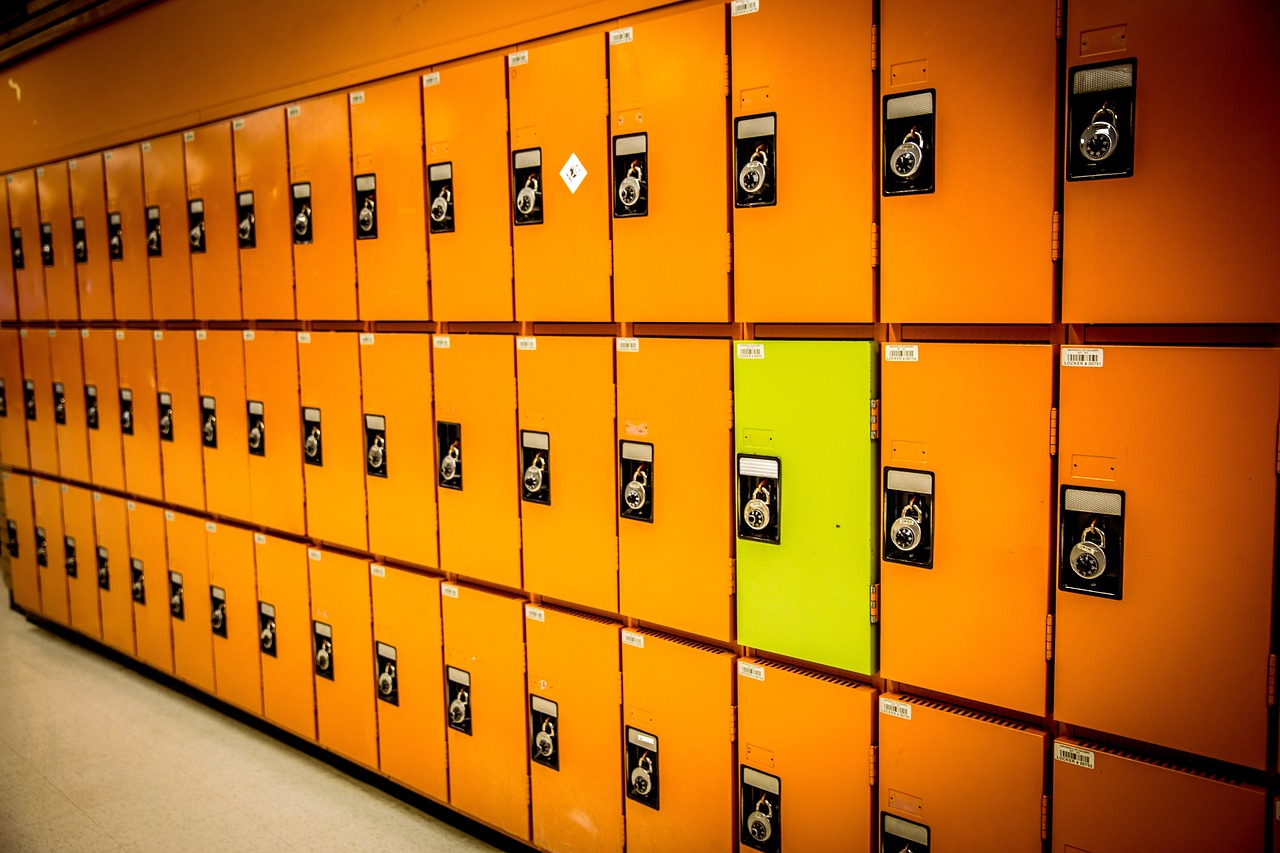
\includegraphics[width=2.08333in,height=1.04167in]{img/unique-1-yellow-locker.jpg}

The best way to contrast with your competitors is to be very Effective AND very Capable -- from your customer's point of view

Unique means Standing out from the crowd.\\


\includegraphics[width=2.08333in,height=1.04167in]{img/be-unique-red-paper-plane.jpg}

\includegraphics[width=2.08333in,height=1.04167in]{gif/stand-out-in-crowd.gif}

Unique means being unconventional.

\includegraphics[width=2.08333in,height=1.04167in]{gif/red-raincoat-in-crowd.gif}

Avoid conventional logic because all your competitors will use that.


\includegraphics[width=2.08333in,height=1.04167in]{img/unique-red-paper-plane-on-black.png}

Test counter-intuitive ideas because your competitors won't.

What is the Best Way to `Stand Out' and Be Unique?

Create the unstoppable chain reaction: Become very Effective, then Build awesome Capability to deliver, And you will be irresistably Unique

So, what does it mean to be ``effective?'' Effective means knowing what creates REAL value for customers - in their terms and having the capability to deliver it upon demand

Effective means\ldots{} Strictly from the customer's point of view. Your efforts must be Useful, or Fulfill a desire, or Solve a problem -- From the customer's point of view

Effective does NOT mean Expedient. Expedient = Quick, Interim or Temporary, Short-term -- often at the expense of the long-term. Putting out fires, often at the expense of the customer

Strangely, the opposite is NOT true: Efficient ≠ Effective. As you become more Effective you will automatically become more efficient.
Productive ≠ Effective

As you become more Effective you will automatically become more productive. But, don't just take my word for it\ldots{} Let's hear what Warren Buffet thinks about Effectiveness in delighting customers

Buffet on the Importance of 'Customer Delight

Some Cold, Hard Facts\ldots{}

\begin{itemize}
\tightlist
\item
  Half of new businesses fail in 5 years.
\item
  By year 10 fully two-thirds are gone.
\item
  Only 10\% make it to 20 years.
\end{itemize}

Studies and surveys also show shocking failure rates for improvement initiatives that can range from 50\% to 70\% or even higher.

If you are ambitious and flexible, this is all good news for you!

\begin{itemize}
\tightlist
\item
  If you become Effective enough,
\item
  If you become Capable enough,
\item
  You will become Unique enough.
\end{itemize}

It's not remarkable that companies fail. It's remarkable that they fail so often, and have for so long!

Obviously, we make the same mistakes over and over again. Otherwise, those grim survival statistics would have improved long ago.

And what about the companies that are just surviving? They are neither fully alive nor completely dead. This is not a laziness problem, or an intelligence problem. Most business owners are very hard- working, and good at what they do. But they're not very good at turning all that hard work into prosperity and a better life.

Where Companies Go Wrong

\begin{itemize}
\tightlist
\item
  They are `Same-As': EACH COMPANY JUST LIKE THE REST. Afraid to be different.
\end{itemize}

`Same-As' companies don't last long in the marketplace. They Copy, Copy, Copy

Everyone from business schools to self-help books continue to tell owners that copying others is the solution to their problems. `Follow-the-Herd' companies don't stand a chance in the marketplace. Woo Hoo! Let's do what everyone else does!

On top of that, most `Solutions' are Incompatible with your existing systems. For example, companies naturally adopt the style of management known as `command-and-control'. Unfortunately, most improvement schemes (and many company goals) are incompatible with this style of management. So, most improvement efforts are doomed from the outset.

So, what's a leader to do?
* Learn to be more Effective, in the eyes of your customers
* Learn to be more Capable in the eyes of your customers
* Learn to be more Unique in the eyes of your customers

These things hardly cost a thing\ldots but, they require a different mindset, a sense of urgency, and the willingness to try new things.
The reward is to become Unique in the marketplace -- which is the Point!

WHAT TO DO NOW?

FIRST\ldots{} Adopt a plain-spoken aim such as ``Our Mission is to Create Happy Customers!'' Lose the corporate-speak, gobbelty-gook jargon. It makes it much harder for everyone to do a great job.

Next\ldots{} learn first-hand what your customers value -- from their point of view.

Next\ldots learn first-hand, what your customers experience when dealing with your company (the good, bad, and ugly).

Management Is Not Very Good at Guessing What Customers Value. So, it PAYS (a lot) to Ask Them Directly.

Case Study: Initially, Dr.~T and her team came up with 23 ideas of how to create more value for her customers. Let's see how they did by themselves\ldots{}

A vizualization of the two dimensions of customer value, the technical dimension and the emotional dimension. In the veterinary services sector

Medicine is high on the Technical and low on Emotional dimentions.
Administration activities are low on both the Emotional and the Technical dimensions.\\
Customer Desires are high on the Technical dimension and the Emotional dimensions.
Customer Frustrations are high on the Emotional dimension and low on the Technical dimension.

This is represented with this graph:

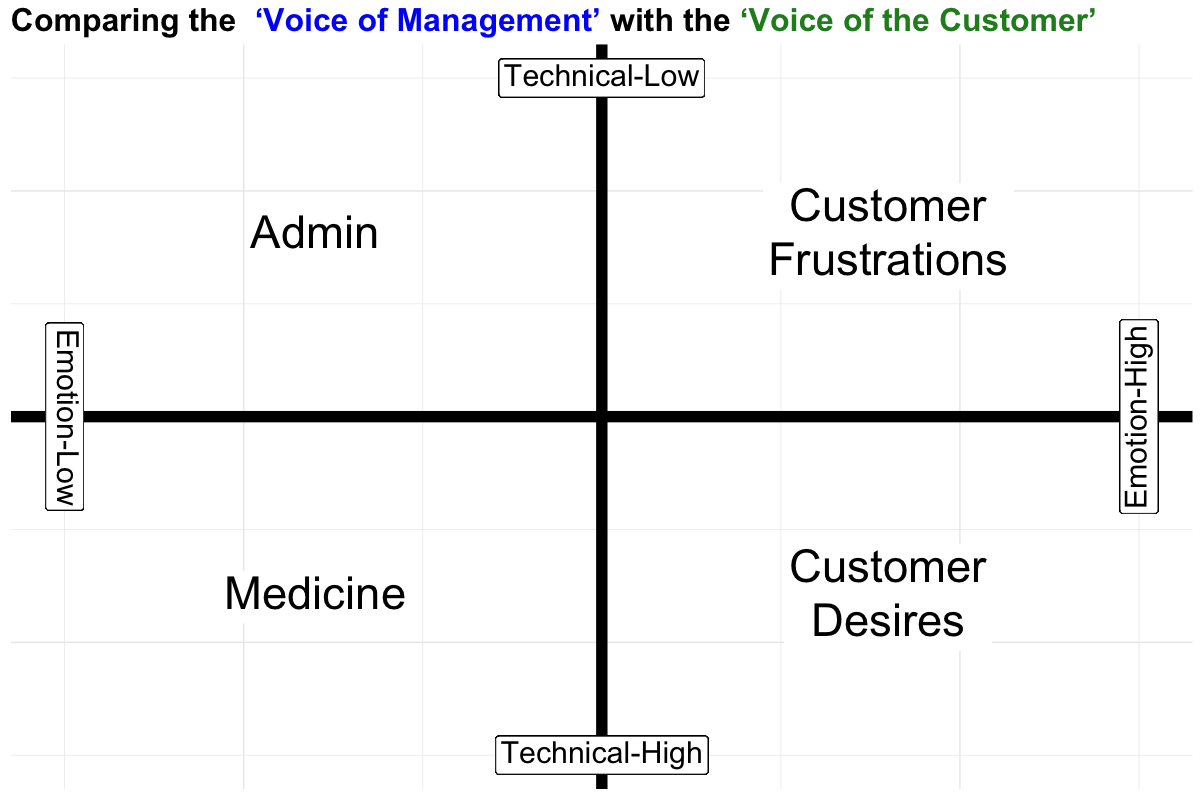
\includegraphics{img/blank-all-4-quadrants.png}

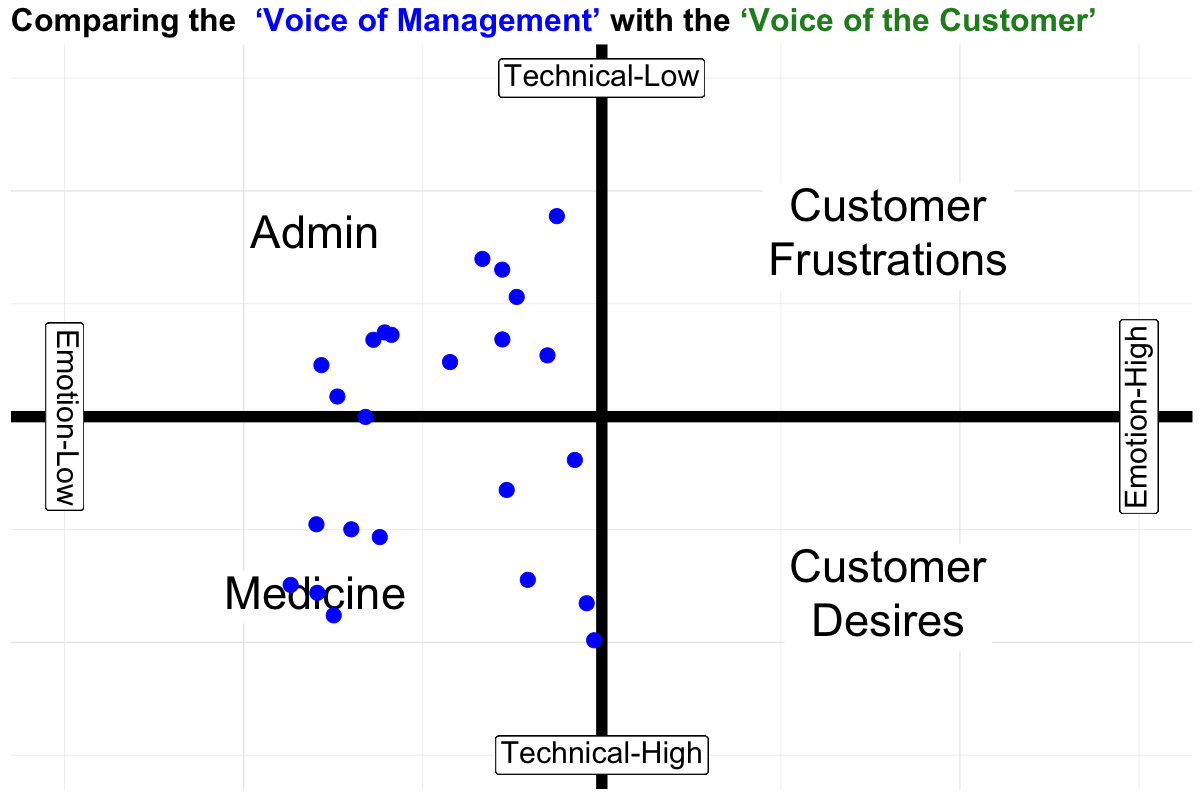
\includegraphics{img/quadrants2and3.png}

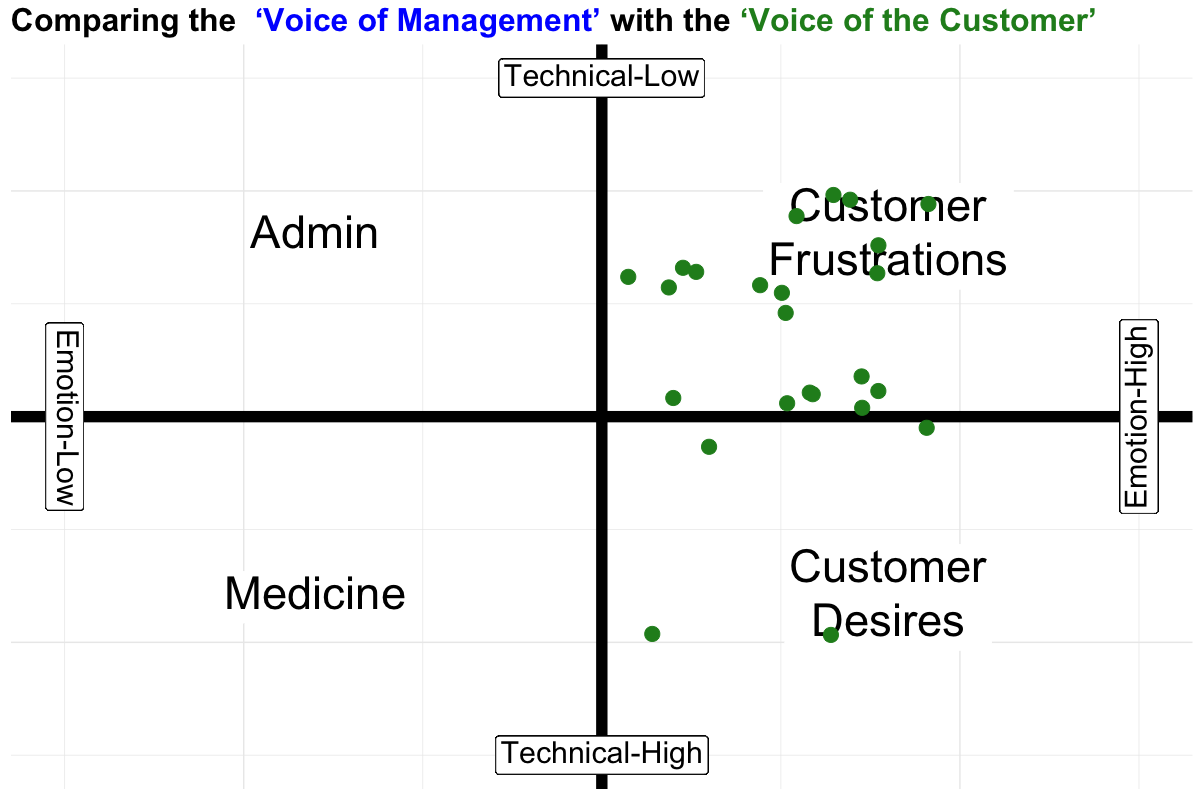
\includegraphics{img/quadrants1and4.png}

\begin{figure}
\centering
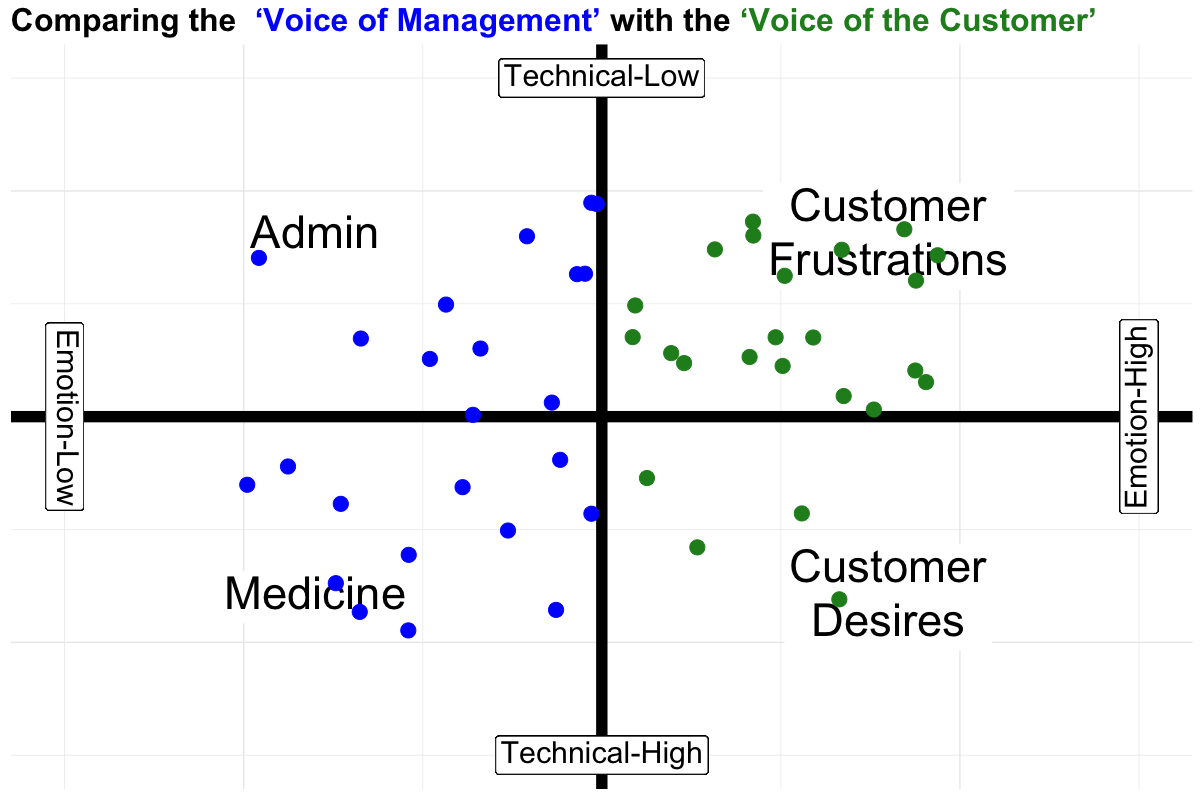
\includegraphics{img/all-4-quadrants-with-dots.png}
\caption{The Value Ideas Compared}
\end{figure}

If there is any way at all Ask Customers Directly! It PAYS (a lot) to Ask Them Directly

Then\ldots create Capability so customers can pull the value they need from you when, where, and how they want to.

Case Study: Stew Leonard's Dairy has mastered the ability to `Listen, then Deliver'

Stew Jr on the Power of Customer Suggestions

Some Things To AVOID\ldots{}

BEWARE OF\ldots{}

\begin{itemize}
\tightlist
\item
  Slogans,
\item
  so-called `best practices',
\item
  Agile,
\item
  Lean or Six-Sigma,
\item
  Mission \& Vision statements full of buzzwords,
\item
  Servant leadership,
\end{itemize}

These are all management fads and they all have one thing in common: they avoid the responsibiltiy of management to create and maintain a system based on Effectiveness and Capability

GUIDING PRINCIPLES for Action

Apply your GUIDING PRINCIPLES daily to get AMAZING RESULTS

GUIDING PRINCIPLE: Focus on measures of Effectiveness \textasciitilde{} Not on measures of Efficiency

When you focus on measures of Effectiveness \& Capability \textasciitilde{} You will automatically be more Efficient and Productive.

To be Unique You Must Be Effective! (EVERY DAY)

To be Unique You Must Be Capable! (EVERY DAY)

If you're looking for a `sure-fire', low-cost way to prosper in the marketplace\ldots{} Become very Unique, and one sure-fire way is to become very Effective and very Capable.

\hypertarget{part-part-iii---inspiration}{%
\part*{Part III - INSPIRATION}\label{part-part-iii---inspiration}}


Arrow-like characters in Unicode:

\begin{verbatim}
Leftwards Arrow: ← &#x2190;
Upwards Arrow: ↑ &#x2191;
Rightwards Arrow: → &#x2192;
Downwards Arrow: ↓ &#x2193;
Diagonal Arrow Up: ↗ &#x2197;
Diagonal Arrow Down: ↘ &#x2198;
Bent Arrow Right: ↪ &#x21AA;
Bent Arrow Left: ↩ &#x21A9;
\end{verbatim}

RED BOX Example of an \textbf{.rmdcaution} block.

GREEN BOX Example of an \textbf{.rmdimportant} block.

BLUE BOX Example of an \textbf{.rmdtip} block.

BLUEVIOLET BOX Example of an \textbf{.rmdwarning} block.

\hypertarget{case-study---stew-leonards-dairy-store}{%
\chapter{Case Study - Stew Leonard's Dairy Store}\label{case-study---stew-leonards-dairy-store}}

This chapter uses long-form video content allowing readers to sit back, listen and watch examples of the key business lessons directly from the entrepreneurs themselves. The duration is listed with the video. A timeline of highlights is provided in the text below. Now, sit back, enjoy, and be inspired!

Every example in this book comes with this caution:

{`Don't copy 'Best Practices'}\ldots{} ~ ~ {`INSTEAD, TEST THEORIES AND PRINCIPLES'}.

The practices and procedures you see in the examples are the creative expression of an underlying principle or theory that is being tested for success in a specific setting.

They represent part of a chain reaction (theory) the company hopes will bring the results they desire. You must understand the chain reaction behind the practice to understand how the idea might help your company.

Remember: Every company is one-of-a-kind. Different owners, people, products or services, machines, methods, measures, marketplaces, and locations. Your setting will always be different, even though you might be in the same industry.

One of the best lessons of an example is: {`TRY NOVEL IDEAS BECAUSE YOUR COMPETITORS WON'T'}

Here's a chain reaction (theory) that describes WHY Stew Leonard's operates the way it does:

\textbf{HAPPY PEOPLE {→} HAPPY CUSTOMERS {→} HAPPY BANKER {→} HAPPY OWNER}

(Where you see {→}, read ``\ldots leads to\ldots)

\hypertarget{background}{%
\section{Background}\label{background}}

Stew Leonard's Dairy Store was `discovered' when it was included in Tom Peters' now-classic book \textbf{\emph{In Search of Excellence}}. Stew Leonard's is an extraordinary business and a real-life example of most key principles found in this book. Namely,

\begin{itemize}
\tightlist
\item
  Simple ideas, taken very, very seriously
\item
  Uses the `Learn, then Provide' strategy to create additional value for everyone
\item
  The creative courage to be different
\item
  Purposeful positioning relative to competitors
\item
  Real empowerment; not the fake variety so popular today
\item
  Treating the business as a system of interdependent parts, not as independent profit centers. All departments work together to accomplish the common mission.
\item
  Don't copy `Best Practices', COPY `BEST THEORIES AND PRINCIPLES'.
\end{itemize}

\hypertarget{guided-media-and-discussion}{%
\section{Guided Media and Discussion}\label{guided-media-and-discussion}}

This example is punctuated with video clips illustrating each aspect described above and contains a concept from which to build a business philosophy.

Timeline Tactic Ordinary Grocery Store Stew Leonard's Note 1 Note 2 Note 3
1:22 No of Items 15000 800 80/20 concept\\
1:55 Customer is Always Right No Yes Customer Satisfaction, customer loyalty, market position Way of life from top to bottom Lifetime Value
3:12 Story\\
4:55 Power of a symbol\\
5:55 Atmosphere Disneyland of grocery stores Customer sayings\\
6:40 Customer testimonials\\
7:55 Happy customers are repeat customers\\
8:22 CEO sets the tone\\
9:10 Cashiers\\
8:35 How to solve budget problems - KPIs\\
10:50 Suggestion box\\
11:10 You better react to these right away!\\
11:16 Our customers tell us what our problems are and we solve them ASAP\\
11:30 The customer that complains is our best friend\\
11:35 Easy to be too busy to ask the customer\\
11:50 Focus groups\\
14:20 Respond, respond, respond\\
15:00 Tap the customer knowledge\\
15:20 Searching constantly for new good ideas Copy ideas; not specifics. Must improve customer experience\\
16:30 New ideas are what this store's made of\\
16:45 Hired for attitude, not specific skills\\
17:30 TRUE empowerment\\
17:50 Training budget 4 times industry avg\\
18:00 Success is becoming yourself at your very best\\
18:20 Team members Org chart diff than industry\\
19:00 Turnover 200\% - 300\% 60\%\\
19:30 Productivity is a result; can't be controlled directly\\
20:15 4 Principles that has made Stew Leonard's so successful satisfy customer, teamwork, excellence, WOW!\\
22:00 focus on the little stuff\\
22:40 ladders of success\\
25:00 Dale Carnegie course for all\\
25:45 Depts working together, not pitted against each other\\
26:40 Better quality = increased profit\\
26:45 KPIs are results, not directly controlled\\
28:00 Empowerment = trust\\
30:00 better today than yesterday\\
31:00 supplier relationships \& technology high quality, high integrity. Like Toyota it's WIN-WIN Better margins by max value
36:00 quality quality quality\\
39:30 Know your numbers (costs, volume, movement)\\
40:20 dept mgrs get lots of info to know what is happening more than other stores in industry\\
42:45 awareness of information leads to awareness of problems which leads to awareness of solutions\\
43:00 long-term thinking; no short-term thinking\\
44:00 Sharing the Philosophy\\
45:35 Leadership\\
48:35 happy people = happy customer = happy banker = happy owner!\\
49:00 profit is regard for getting all the customer stuff right\\
49:28 Filming the wrong things!\\
Conviction and passion\\
Innovation\\
Management by being flexible to change\\
People have opportunity to reach their potential\\
57:15 Stew's lament

Case Study: Stew Leonard's Dairy has mastered the ability to `Listen, then Deliver'

Stew Leonard's Formula for Success

Arrow-like characters in Unicode:

\begin{verbatim}
Leftwards Arrow: ← &#x2190;
Upwards Arrow: ↑ &#x2191;
Rightwards Arrow: → &#x2192;
Downwards Arrow: ↓ &#x2193;
Diagonal Arrow: ↗ &#x2197;
Diagonal Arrow: ↘ &#x2198;
Bent Arrow: ↪ &#x21AA;
Bent Arrow: ↩ &#x21A9;
\end{verbatim}

RED BOX Example of an \textbf{.rmdcaution} block.

GREEN BOX Example of an \textbf{.rmdimportant} block.

BLUE BOX Example of an \textbf{.rmdtip} block.

BLUEVIOLET BOX Example of an \textbf{.rmdwarning} block.

\hypertarget{case-study---mattress-mack}{%
\chapter{Case Study - Mattress Mack}\label{case-study---mattress-mack}}

This chapter uses long-form video content allowing readers to sit back, listen and watch examples of the key business lessons directly from the entrepreneurs themselves. The duration is listed with the video. A timeline of highlights is provided in the text below. Now, sit back, enjoy, and be inspired!

Every example in this book comes with this caution:

{`Don't copy 'Best Practices'}\ldots{} ~ ~ {`INSTEAD, TEST THEORIES AND PRINCIPLES'}.

The practices and procedures you see in the examples are the creative expression of an underlying principle or theory that is being tested for success in a specific setting.

They represent part of a chain reaction (theory) the company hopes will bring the results they desire. You must understand the chain reaction behind the practice to understand how the idea might help your company.

Remember: Every company is one-of-a-kind. Different owners, people, products or services, machines, methods, measures, marketplaces, and locations. Your setting will always be different, even though you might be in the same industry.

One of the best lessons of an example is: {`TRY NOVEL IDEAS BECAUSE YOUR COMPETITORS WON'T'}

Jim McInvale, founder of Gallery Furniture in Houston, TX, has mastered the ability to `Listen, then Deliver'

New Management Methods Transform Gallery Furniture into Greatest Furniture Store in World

2:08 My less than illustrious background

currently the business in 1991 our sales figures were 45 million dollars we only have one location 30,000 square feet

our sales average per square foot is \$1,600 whereas the industry average is about 125

we have the highest sales per square foot ratio in the world the industry average of sales of inventory turnover is 2.5 times a year we turn our inventory about 25 times a year which is also the highest in the world

so we've done a few things right but the biggest thing we've done right is Gallery furnitures transformation from competition to cooperation. cooperation works and

8:22 Sameday delivery

Gallery Furniture is a 30,000 square foot retail furniture
store servicing the medium high priced furniture market in Houston Texas

from the beginning we were able to differentiate ourselves by offering him same-day delivery of furniture. you can come to our furniture store anywhere
from 8 o'clock in the morning ten o'clock at night seven days a week and buy furniture. say you buy the furniture 10 o'clock at night we still deliver it the same day. on any given Saturday or Sunday we do up to 300 same day deliveries. people buy the furniture today and they do get it delivered within three or four hours.

we have set a benchmark for all the world in immediate
delivery of furniture. that has always been our cutting edge improvement where we had a edge over our competitors. you could buy it today and get it today immediate gratification

9:11 Management structure
Gallery furnitures also had a very conventional management structure with the boss me at the top and everybody else down throughout the organization. I was taught this conventional management structure at the University of Texas and
that's the way I thought it was supposed to be. however management which was me over the past 10 years I became very frustrated. one thing we were very good at measuring was the number of customers coming into the store on a daily basis say we had a hundred customers and we also paid all of our salespeople a very high commission sales rate about double what the industry standard was. the objective was to make the sale by any method as long as it was legal. and people came in we did all sorts of used-car tricks to make the sale. however over the past ten years we noticed that our store closing percentage, the number of customers who bought versus the number of total customers for the day, never got above forty percent no matter how many extra incentives were offered. contests were started to threats were made and so I was very frustrated because I knew if the business was going to grow we had to get our closing percentage over 40 percent. now keep in mind that forty percent was an outstanding closing percentage because the industry average is 20. however we did want to continuously improve so I kept searching and trying to find a way to get the closing percentage over 40 percent but nothing ever worked and I was very very frustrated. so management (which was me) came up with a brilliant idea. I decided the best way to get the closing percentage up was to get the superstars in front of more customers

10:45 Monthly contest

At that time we had 80 salespeople so we decided we'd have a monthly contest and at the end of the month of August the top 10 producers out of those 80 for the month of September, the top 10 ranked one through 80 the top 10 for the month of September could take as many customers as they liked. you know, they wouldn't have to go in a batting order type basis like everybody else would. They'd be up in front of the customers all the time. this would double or triple their income and the idea was it would raise the closing percentage by getting the superstars in front of more customers. this was Jordan judging performance using arbitrary goals or figures and what happened was this didn't work either. this was a classic case of `tampering'. the ten or so people who were lucky enough to win come to my buckets were embarrassed all throughout September because they get preferential treatment over their friends and the other seventy people felt like losers or failures. in this zero-sum game we were playing.

12:29 Judging performance - total blindness to the customers concerns

fought the traffic to and from Gallery Furniture in my daily commute on the North freeway in Houston Texas
16:00 Gallery furniture had been lucky and successful in spite of my bad management practices which crushed people in their intrinsic motivation.

20:06 Removing quotas - Everybody told me it wouldn't work

20:34 Ressults

18 months later people don't do less work they actually do more

they're eager to jump in and prove their worth and contribute to the good of the whole

21:44 Business as a system

I no longer look at individual sales figures I haven't looked at individual sales figures in over 14 months. I could care less. What really matters is how is the entire business doing? Are we taking care of the customers, are we taking care of the employees, are we taking care of the community, are we making a profit? the organization as a system dr. Deming is
22:14
view of the world now I've come to realize that people are going to have great muscles are going to have very four months it's part of the variation
22:21
of dr. Deming teaches and as we have continued to improve the business people have become improvement project players
Improvement project players
22:32
further learning where they too can fit in and using their special talents to
22:37
contribute to the good of the system that is probably the most amazing change people learning how to do different jobs
22:43
and contribute to the good of the system and the bottom line of the whole business is what business are we in

we
22:49 We thought we were in the business of selling furniture; we're actually in the business of delighting customers. there are 300 retail locations in Houston Texas where people can buy furniture but there's only one that really delights customers and we believe it's us. the purpose of the business is to delight customers nothing else

The great American phrase of It's not my job has totally disappeared

23:42 Customer needs and concerns
learn how to identify customer needs and concerns and take those into the reality of the business and that's what we've
23:47
been able to do in the last 18 months identify customers needs and concerned because people
23:59
now perform for the good of the system they do all different types of jobs
What do sales people do
24:05
before we had 80 people what are the 80 sales people used to do sales nothing
24:10
else other than that they sat and read the newspaper and smoked cigarettes today what do sales people do they do
24:16
sales they do inventory control they move the furniture for the displays in the store continuous housekeeping they
24:24
supervise our playground we Han now have but cut based upon the suggestion of one of our mothers who works there at the
24:30
store she said why don't you put in a playground we put in a huge playground bigger than any playground a McDonald's and we have our people now supervise the
24:37
playground for the kids what are the furniture store do you know of where kids cry when they have to leave
24:49
we prepare the furniture for the delivery we frame sheetrock finish and paint we display the rooms we stripe the
24:55
parking lot we do whatever it takes what else do they do they act in the
25:01
commercials they do data processing they drive the trucks they coordinate the service calls they paint the store they
25:07
do decoration they provide store security they direct customer traffic on Saturdays and Sundays when it's too busy
25:12
they answer the phone they make popcorn and they go on deliveries one of the big changes we made was before we had
25:17
contract delivery drivers doing the deliveries most contract delivery drivers are people that live from hand
25:23
to mouth it was very frightening to some of the our customers to get a knock on the door and look out the door and see
25:29
two weeks showing up at their house at 10 o'clock at night to deliver furniture
25:34
and we got a lot of feedback from the customers with a big crime wave in Houston that they didn't want these semi
25:41
vagrants delivering the furniture to them that's the way it's done in the industry so we decided to have our own quality salaried salespeople do the
25:48
deliveries it cost us a lot more but what are the benefits and customer satisfaction I'm fixing to show you what
25:53
the benefits are then our own quality sales people do the deliveries what does
25:58
that enable them to do they see the business totally different than one way of just selling now they go into customers home and they see how the
26:04
furniture actually fits in the customers home and they see how they can sell that customer more furniture once they get in
26:09
their home what about the bottom line
Hard numbers
26:18
everybody says this is wonderful in theory but can you give me any hard numbers any examples I said yes I can
26:24
give you lots of hard numbers lots of examples the number of visitors you can see it's in control purple line is 1990
26:32
the Aqua Line is 1991 very consistent in October of 1991 our customer traffic
26:39
went down versus the previous year in the same month for the first time ever because of a crime wave in Houston and
26:45
people were literally afraid to go out after 6 o'clock at night but still then our because of our cooperative system
26:51
sales went up that's the number of visitors please contrast that graph
26:58
with the number of visitors making a purchase the green line is 1990 in the
People have learned how to
27:04
red line is 1991 it went from 40 percent to about 55 percent the highest in the
27:10
world and to make a 15 percent increase when you're always already the best was a tremendous improvement people have
27:17
learned how to work together here's a typical example about a month ago we had two very wealthy of wealthy husband and
27:25
wife and their children come in from Mexico City they just bought a new summer home in Houston they wanted to furnish the home they got to the store
27:31
about 9 o'clock at night and one of our Anglo sales persons greeted these customers he knew these people were very
27:37
uncomfortable talking English and he knew they wanted to speak to somebody who could speak their native language
27:42
which was Spanish so he went and got one of our female associates a nice young lady only been with us about six months
27:48
to help these people they were so delighted to have somebody that worked with them they spoke their language and understood what they wanted
27:53
they ended up an hour and a half later spending \$40,000 before that salesperson would never have turned over that
27:59
customer and they would have walked without buying anything store closing
Store closing percentage
28:08
percentage has been a steady climb up over the last 18 months delivered
28:15
furniture we were supposed to be in a recession the blue line is 1989 the yellow line is 1990 and the green line
Recession
28:22
is 1991 and so far this year we've been too busy taking care of customers to make many charts but I will show you the
Results
28:34
first quarter results you want to manage by the numbers here they are first
28:39
quarter results 1991 gross sales 10 million 236 net income 1 million 1 2 -
28:46
first quarter results in 1992 sales almost the same 10 million to 54 net
28:52
income 1 million 4 6 3 increasing that income by \$340,000 what I'm telling you
28:58
is cooperation works competition doesn't
Cooperation vs Competition
29:10
cooperation versus competition cooperation Christine works Angie better morale more responsive to the customers
29:16
competition is inefficient creates bad feelings and productive and unfair competition you see I believe we've been
29:23
sold down the river in this country on something called competition we think it's good I win you lose I learned how
29:28
to compete playing football at the University of Texas in 1969 in 1970 when the long runs won 30 straight games two
29:34
consecutive national championships there were some great competitors on the team two of my best friends in Houston teach
29:41
young people how to compete in the ioniq fields one's name is John Jenkins head football coach University Houston the
29:47
others name is Bela Karolyi world's finest gymnastics coach coach to the girl you saw in Time magazine in
29:54
Newsweek the last two weeks her name was Kim zamesca of Houston Texas she didn't win the Olympic Games labelled her a
30:00
failure I don't think she was a failure do you competition what has it done to
30:09
us but a gallery furniture thanks to dr. Demmings request we change we transformed transformation and
Transformation Management Thinking
30:18
management thinking before the way I was taught focus on individual events who's to blame find somebody
30:24
now we view the company as a whole we don't focus on individual events we focus on improving before we said
30:30
goodbye to below every staff members now we view the employees as asset the biggest and only asset of the company
30:35
before no education the turnover is to hide today return on investment mentality how can we invest lots of
30:41
money in our best asset our people before I became very frustrated because people didn't get my hyperactive message
30:47
now I have learned now I have learned
30:53
that different people learn in different ways and you know what other amazing discover we have made people buy in
30:59
different ways different things motivate people to buy and I'll tell you about that in just a few minutes here before
31:05
we beat and dwell on problems odd nauseam an issue eating so every time a problem happened it was we judged it to
31:10
be a mostly it was a special cause we thought was a common cause would issue a new rule now it's made my job harder
31:17
must do fire prevention not firefighting let's think about how to improve the system and that's a lot harder than
31:22
doing knee-jerk reactions before we ignore the potential of competent people today we find out that everybody has lots to
31:28
contribute and will contribute if only given a chance additional benefits
31:35
people are happier on the job better morale and attitude people see the business as a whole system there's no
31:41
more infighting between departments all departments work together for the good of the business before we had a system
31:47
where we had four or five professional furniture buyers and set in an office all day long the only people they saw
31:53
with the vendors from the different manufacturers and they bought the furniture we no longer have professional
31:58
furniture buyers our buyers are the retail salespeople who are there on the floor on a daily basis interacting with
32:04
the customers and they buy based upon what the customers tell them to buy listen to the voice of the customer it's
32:10
worked a whole lot better now people are eager to volunteer ideas and opinions to make the business better what we're
32:17
trying to do is to create an atmosphere where people are willing to take high risk and reap the high rewards in most
Take High Risk
32:23
businesses we're stuck over here on this side of the distribution low risk cya move up through doing nothing be safe
32:30
and mediocre we're trying to get people out on the right-hand side of the distribution high-risk high-reward in
32:36
sales merchandising decorating whatever it might happen to be take a risk what's
32:42
going to happen out on that far side of the distribution is we're gonna strike out a lot the other thing it's gonna
32:47
happen is we're gonna hit a lot of home runs to come up with a lot of innovative ideas the problem with the retail
32:52
furniture business is most retailers in the furniture business haven't had a new idea in 50 years and that's why our
32:58
industry our share of consumer disposable dollar used to be three and a half percent and now it's about 1.2
33:03
percent and steadily going down so if we're going to improve and save our little industry we have to take some
33:09
innovative high-risk high-reward type of chances
33:16
we change from a system that caused this type of reaction from the customer after
Change From A System
33:22
listening to your commercials for years I expected to be treated to a pleasant buying experience instead I dealt with
33:28
pushy salespeople in a finance group it became aggravated when it didn't purchase their way that's the way it
33:33
used to be in the Commission days so we decided we would change and listen to the voice of the customer and that's
33:39
really what the business is all about and here's what happened
33:48
David was our salesperson he was extremely nice and helpful and everyone as a whole was extremely nice and polite
33:53
I think changing your salespeople from commission to salary was an excellent idea
33:58
delivery the furniture went well the delivery guys were nice and efficient Thanks that's the difference between
34:04
competition and cooperation the
34:12
salesperson and the finance person were great Leslie a new heart I really loved the insurance coverage also on the
34:17
tables Leslie told me about Newhart was the greatest salesperson I've ever seen all my money will be spent at Gallery
34:23
Furniture from now on Newhart's mother wrote that one
Gallery Furniture
34:32
see tom was great there was never any pressure while giving us lots of valuable insight and information many
34:37
thanks I'll be back with lots of money we look forward to that one you see
34:48
before if a customer was browsing you didn't spend your time with him eating waste your time he didn't tell him he just dropped him and got somebody who
34:54
wanted to buy something that's the big difference
Quality
35:02
prices are excellent the quality is excellent sales people are excellent you have an all-around excellent operation
35:08
and gallery furniture compliments and best wishes we used to get 10 or 15 negative letters a month now we get about 50 of these a
35:17
week and I have to believe that long term it's going to pay big-time dividends for the business
35:29
my wife and I were treated as valued customers even though our purchase was not large our salesperson was courteous
35:34
knowledgeable and not high-pressure will be back give me an example of that we had a customer two weeks ago went to four different furniture stores trying
35:40
to buy a bed frame full-size bed frame cost \$22 salesperson if they're making
35:49
5\% Commission makes a dollar on that sale nobody would take the time at the four of the stores to sell it to her she
35:54
became very agitated she came to our store our guy took a lot of time sold the 22 dollar bed frame she was very
36:00
happy on the way out she bought a six thousand dollar dining room set Sam was
Sam Wood
36:13
such a good salesperson at a terrific wheelchair operator in Sam we thank you so much for the service you gave my 92
36:19
year old mother Muriel from Arkansas before Sam Wood had no incentive to help
36:25
that lady because it wouldn't be paid for it so he would have thought now they treat the people like human beings
George McIngvale
36:35
George is a very pleasant person she was very helpful I don't think we would have bought the nice furniture wasn't for her
36:40
thanks a lot and the list goes on and on and this is really the business we're in is delighting people where they go back
36:46
to their job their office their factory or the government office where they work and they tell people what how well they
36:52
were treated at our store now when customers come in the first thing we do is give them an ice cream bar we have
36:58
face-painting that our sales people do for the customers we have the playground we have popcorn we've got all sorts of
37:04
things going on because we want to make it a fun atmosphere where people will come back a negative experience they will enjoy and cherish the experience is
37:11
as important as the product to the customer
37:19
our truck broke down behind the store we came up here to use the phone we were treated like family like this the
37:25
service was just extremely nice I couldn't ask for more things what happened is people work together and
37:30
they're concerned about the customers and that's the business were in dr.
Dr Deming
37:39
Deming says Institute leadership the aim of supervision should be to help people in machines and gadgets do a better job
37:45
supervision of management is in need of overhaul as well as supervision of production workers in our case it was
37:51
supervision of management
Dr McIngvale
38:00
role of a manager of people a manager and as people understand the meaning of a system and how the work of his group may support these aims all departments
38:07
understands how they're going to support the aim of the rest of business people asked us all the time do we make any
38:13
money on our delivery service I don't care if we make money on the delivery service it's irrelevant what matters is we're delighting customers the manager
38:20
works in cooperation with preceding and following stages to optimize the effort of all stages he understands people are
38:26
different from each other he's an unceasing learner he's a coach and counsel not a judge he understands a
38:32
stable system study results to improve his work another aim is learned if
38:37
anybody's outside the system we need a special help he creates trust he does not expect perfection he listens and
38:43
learns without passing judgment we had a sales person come to work for us about
38:49
six months ago and after three months I learned that he was an epileptic and he
38:55
had a seizure in the store on a busy day upset a lot of people everybody said we shouldn't have him there we kept him
39:01
he's now one of our best and most loyal and / employees does a terrific job because we didn't pass judgment on him
Who is the leader
39:14
who is the leader s is the best leaders that people do not notice their existence the next best that people honor and praise and next to people fear
39:20
the next people hate when the best leaders work is done that people say we did it ourselves
39:25
productivity increases in the old commission days we had the high power used car salesperson
39:32
if it did \$3,000 in Saturday they had a great day now we have kids 22 and 23
39:38
years old with no previous sales experience because we improve the system on any given Saturday Sunday to do 10 and \$12,000 that's a four to one
39:45
increase we haven't improved everything in the business because people learn how to work together
Intense cooperation
39:55
intense cooperation think about it everybody wins is a long and arduous task but it can transform American
40:00
business we must saturate every area every activity we must again begin right now even we're trying now to cooperate
40:07
with our competitors a difficult thing to do with something we could benefit all of us just to give one example we're
40:13
now pooling our trucks from California with ourselves and our competitors is enabled both of us to bring down our
40:19
freight rates by about 5\% we have learned in the furniture business we're not competing with each other we're
40:24
competing with other people for the consumers disposable dollar if we work together everybody can have more quality
A long hard climb
40:36
and innovation been a long hard climb at Gallery French if I told you was easy there were no problems I'd be lying to you there's been lots of problems but
40:43
certainly the efforts been worth reward
Choice
40:51
Gallery Furniture we had a choice to make which path to take we could keep doing our quick roads to quick returns
40:57
over here crush people made a lot of money doing that we're very very profitable we decided to make the change
41:04
but after going ours and listen to the brilliant people that around dr. Deming I decided to take the long-term route to
41:10
Deming prosperity and that's what we did what happened was a dimming chain
41:16
reaction we improved quality we're able to decrease our cost our costs have gone
Improved Quality
41:23
down tremendously we're able to improve our productivity like I said before people do 3,000 on a Saturday now to do
41:29
10 to 12,000 we're able to decrease our prices to the retail customers we're able to increase the market for
41:35
everybody but by doing more advertising we've certainly been able to stay in business provide jobs and get more jobs
41:40
for our community and get a return on investments to the stockholders in other words winning is everything but only if
41:49
everyone wins dr. Deming also taught us
Group Process
41:56
something called a group process plan-do-check-act before we'd make these massive changes without any thought now
42:02
we do it on a small scale we planted plan a change angel aimed at an improvement carried out on a small scale
42:08
what are the results what did we learn if it worked implemented company-wide if not do it all again
42:13
if it ain't broke improve it that's what we're trying to do is constantly improve everything we do in the business so the
42:19
business gets better and everybody can have more fun and make more money isn't that what it's all about you see there's
Lone Ranger
42:30
a great big myth in this country that the American West was settled by the Lone Ranger type manager the hero riding into town on the big white horse solving
42:37
all the problems by himself however that's simply not true the American West
42:43
was settled by people like you and I working together to raise the barn together in harmony
42:49
managers employees educators community raising the barn together people working
The American West
42:55
together so that everybody can win like the kids doing Special Olympics and what's wrong with that about six months
43:02
ago you saw as President Bush mr. stimple of General Motors mr.
43:07
Iacocca of Chrysler mr. poling afford with Japan hat in hand asking him to ease up on us in the automobile business
43:13
why are they head of us in this critical industry very simple because they work
43:18
together business government employees educators they all work together for the good of the community and what's wrong
43:24
with that we used to work together in this country but we lost sight of it none of us in this room were taught
43:31
courses on cooperation in college however I believe that is what we must do recently I attended a chamber
43:38
commerce meeting in Houston I sat next to a friend of mine named Joan I hadn't seen her for about six months on another 11 year old son named Sammy loved the
43:45
sport of roller skating I said Joan how's Sammy doing in rollerskating she
43:50
said I didn't you hear I said hear what she said he quit and I was very shocked
43:56
I said why'd he quit I said I know he loved the sport so much he did it three or four hours every day after school why in the world would he quit she said well
44:04
he went to the Nationals down in Florida last month and when he didn't win the coach yelled at him so much he decided
44:09
it just wasn't worth it is that really the way it has to be why can't we learn
44:16
how to work together so that the business wins the community wins everybody wins
44:22
the last thing I'd like to say about quality improvement is another challenge the youth of America recently I was in
44:31
Los Angeles we gave away 250 sets of mattresses to the people in the 77th Street police station at Crenshaw where
44:38
the riots were as I drove to that neighborhood it was incredible looked like a war zone and I thought to myself
44:44
why did all this happen was the fault of the court system the police was the fault of the kids the rioters no it was
44:51
probably the fault of business people like you and I because we got so caught up in making money we forgot to Linda
44:58
not a handout but a helping hand to these kids be they black white red or yellow and teach them that they too through hard work dedication and a
45:04
commitment to cooperation can live the American dream so that everybody can win
45:10
winning is everything everyone wins thank you very much {[}Applause{]}
45:38
thank you thank now entertain questions there's a microphone in the in the
45:44
middle if some of you'd like to ask a few things about how to pick up mints
45:50
and other other things hi Jim thanks for
45:55
your remarks I'd like to hear a little bit about how you worked with educating yourselves peoples you got ready to change the compensation system in
46:03
particularly those that perhaps have been in that system for saf 35 years and really were winners yeah we my father
46:09
was my father 68 years old he's our sales manager at the store he's a great
46:14
guy but he was brought up on the incentive Commission program he was very much against what we were trying to do as were a lot of the other quote heavy
46:22
hitters or superstars so what we did was we bought the Deming Library videotapes and we'd had a class with all of our
46:29
employees for two hours every day for 15 weeks my wife put together the training course we started with tape one and we
46:36
watched it did the workbook and we went all the way through the end and one of the most poignant moments and that whole
46:41
thing was when one of the people who was dead set against it he was making a lot of money and absolutely destroying the
46:48
business he was out only for his own good we're in that meeting room one day watching the tapes and dr. Deming was
46:55
talking about how life begins with intrinsic motivation and gradually drive it all out to life ends and this person
47:02
was sitting next to me and he it was wrenching and I knew he was very unsettled during the we watched the tape
47:08
we got out outside as we finished walking to the car I said Pete what's the problem he said well as I was
47:15
watching that tape I realized what I was doing and I said what's that he said well my little girl in the fifth grade
47:21
is very smart she made straight A's and we've labeled her genius brilliant achiever great kid etc etc he said our
47:29
little girl in the fourth grade makes B's and C's and we labeled her dumb stupid underachiever and we're totally doing what he exactly
47:36
what he said in the tape and that turned him around and then you know just gradually through the education and
47:42
talking about the time they were the last one in gym class picked to play basketball talking about the time they
47:48
had to stay home for the prom or whatever they began to see this rate rating and ranking of people is stupid
47:53
and now 18 months later they see up and down up and down they see that people
47:58
have good months and bad mice are starting to learn about variation and they see that the system is in control
48:03
and improving the system is the only possible way to improve the business yes
48:08
sir Jim dick Townsend Ann Arbor Michigan how do you compensate your salespeople now
48:14
your staff and how do you decide what level of compensation over a period of years first year they make \$600 a week
48:20
second year 650 third year 700 goes up to \$1,000 after 10 years and that's it
48:26
and we have sales leaders who have a responsibility for managing 8 to 10 people they make more money but they
48:33
work more hours they have more responsibility they're more in it they're in a sales role but also in a managerial role so they make more money
48:39
than the salespeople but they have a lot more responsibility there are some other furniture stores and car dealerships
48:44
that have tried this type of thing and failed at it I was listening to dr. Deming a couple months ago and he said
48:51
the key thing is you have to keep making it happen and that's what we've done we keep managing and leading people and
48:57
directing people it's not a matter of saying feel good guys you're now out there on salary you have at it we manage
49:03
we direct we train we do all the things we used to do only we now we do it better there's no profit participation
49:10
we have a gain sharing property sharing program we distribute 20\% of the company profits every quarter to the people
49:15
based upon the profitability of the business and the proper training is based solely upon the number of hours that you work the quarter it doesn't
49:22
matter what job you do whether you're a truck unloader or the highest-paid manager everybody shares equally in the
49:28
gain sharing proper change what we're trying to do is make a statement that everybody's job is important to the good of the business thank you Jim
49:39
other questions thank you very much
49:44
there's one back there
49:55
do you kind of hide your candle under a bushel an hour you find trouble
50:00
resisting the temptation to go out and tell the other people in that Houston area how they might improve their
50:06
business oh we tell a lot of them if they don't want to hear it so that's fine you know they want to argue about
50:11
it and say it'll never work and we try to work with people if they want to
50:17
change and change this system as far as I'm concerned our business will is so
50:26
much more profitable so much more easier to manage now that we've worked together rather than the way it used to be so
50:31
another little benefit is our cancellations have been cut by 75\% since
50:39
we went to a salary system because they don't sell people something they didn't need
50:52
thank you very much
51:02
you

Arrow-like characters in Unicode:

\begin{verbatim}
Leftwards Arrow: ← &#x2190;
Upwards Arrow: ↑ &#x2191;
Rightwards Arrow: → &#x2192;
Downwards Arrow: ↓ &#x2193;
Diagonal Arrow Up: ↗ &#x2197;
Diagonal Arrow Down: ↘ &#x2198;
Bent Arrow Right: ↪ &#x21AA;
Bent Arrow Left: ↩ &#x21A9;
\end{verbatim}

RED BOX Example of an \textbf{.rmdcaution} block.

GREEN BOX Example of an \textbf{.rmdimportant} block.

BLUE BOX Example of an \textbf{.rmdtip} block.

BLUEVIOLET BOX Example of an \textbf{.rmdwarning} block.

\hypertarget{case-study---dr.-ts-animal-hospital}{%
\chapter{Case Study - Dr.~T's Animal Hospital}\label{case-study---dr.-ts-animal-hospital}}

This chapter includes long-form narrative content. I worked with Dr.~T during the improvement projects described here and can attest to these results. The names, locations, and some of the particulars are changed to protect the privacy of the business, owners, and employees. Now read, enjoy, and be inspired!

Every example in this book comes with this caution:

{`Don't copy 'Best Practices'}\ldots{} ~ ~ {`INSTEAD, TEST THEORIES AND PRINCIPLES'}.

The practices and procedures you see in the examples are the creative expression of an underlying principle or theory that is being tested for success in a specific setting.

They represent part of a chain reaction (theory) the company hopes will bring the results they desire. You must understand the chain reaction behind the practice to understand how the idea might help your company.

Remember: Every company is one-of-a-kind. Different owners, people, products or services, machines, methods, measures, marketplaces, and locations. Your setting will always be different, even though you might be in the same industry.

One of the best lessons of an example is: {`TRY NOVEL IDEAS BECAUSE YOUR COMPETITORS WON'T'}

Here's a chain reaction (theory) that describes WHY Dr.~T's Animal Hospital operates the way it does:

\textbf{HAPPY PEOPLE {→} HAPPY CUSTOMERS {→} HAPPY BANKER {→} HAPPY OWNER}

(Where you see {→}, read ``\ldots leads to\ldots)

Arrow-like characters in Unicode:

\begin{verbatim}
Leftwards Arrow: ← &#x2190;
Upwards Arrow: ↑ &#x2191;
Rightwards Arrow: → &#x2192;
Downwards Arrow: ↓ &#x2193;
Diagonal Arrow Up: ↗ &#x2197;
Diagonal Arrow Down: ↘ &#x2198;
Bent Arrow Right: ↪ &#x21AA;
Bent Arrow Left: ↩ &#x21A9;
\end{verbatim}

RED BOX Example of an \textbf{.rmdcaution} block.

GREEN BOX Example of an \textbf{.rmdimportant} block.

BLUE BOX Example of an \textbf{.rmdtip} block.

BLUEVIOLET BOX Example of an \textbf{.rmdwarning} block.

\hypertarget{case-study---jims-framing-business}{%
\chapter{Case Study - Jim's Framing Business}\label{case-study---jims-framing-business}}

This chapter includes long-form narrative content. I worked with Jim from inception of the business until its closure several years after the `Housing Boom and Bust' in America and can attest to these results. The names, locations, and some of the particulars are changed to protect the privacy of the business, owners, and employees. Now read, enjoy, and be inspired!

Every example in this book comes with this caution:

{`Don't copy 'Best Practices'}\ldots{} ~ ~ {`INSTEAD, TEST THEORIES AND PRINCIPLES'}.

The practices and procedures you see in the examples are the creative expression of an underlying principle or theory that is being tested for success in a specific setting.

They represent part of a chain reaction (theory) the company hopes will bring the results they desire. You must understand the chain reaction behind the practice to understand how the idea might help your company.

Remember: Every company is one-of-a-kind. Different owners, people, products or services, machines, methods, measures, marketplaces, and locations. Your setting will always be different, even though you might be in the same industry.

One of the best lessons of an example is: {`TRY NOVEL IDEAS BECAUSE YOUR COMPETITORS WON'T'}

Here's a chain reaction (theory) that describes WHY Dr.~T's Animal Hospital operates the way it does:

\textbf{HAPPY PEOPLE {→} HAPPY CUSTOMERS {→} HAPPY BANKER {→} HAPPY OWNER}

(Where you see {→}, read ``\ldots leads to\ldots)

\hypertarget{part-part-iii---implementation}{%
\part*{Part III - IMPLEMENTATION}\label{part-part-iii---implementation}}


\hypertarget{exploring-listen-then-provide}{%
\chapter{\texorpdfstring{Exploring {`Listen, then Provide'}}{Exploring `Listen, then Provide'}}\label{exploring-listen-then-provide}}

{MOTIVATION}
{+}
{ASPIRATION}
{+}
{VALUE CREATION}
{+}
{COMPETITIVE STRATEGY }
{+}
{MARKET TACTICS}
{+}
{PHILOSOPHY}
{+}
{OPERATIONS}
{+}
{CUSTOMERS}
{+}
{SOME LUCK}
{=}
{SUCCESS}

When you choose the {`Listen, then Provide' strategy}, marketing for you is the process of:

\begin{itemize}
\tightlist
\item
  understanding customer needs and desires and
\item
  then creating products or services that satisfy those needs,
\item
  promoting,
\item
  and delivering those products or services,
\item
  in a way that benefits both the customer and the business (win-win).
\end{itemize}

This involves a combination of strategic planning, market `research', product and service development, pricing, promotion, distribution, and customer relationship development.

Here's a brief description of each element:

\hypertarget{understanding-customer-needs-desires}{%
\section{\texorpdfstring{\textbf{Understanding Customer Needs \& Desires}}{Understanding Customer Needs \& Desires}}\label{understanding-customer-needs-desires}}

Effective marketing begins with gaining a deep understanding of what customers want, their preferences, and their pain points.

It takes a strong ethical commitment to customers to actively listen to them, even when their feedback might be challenging or critical. It also takes commitment to customer welfare to change and adapt your strategies based on their evolving needs and desires.

\hypertarget{design-product-and-service}{%
\section{\texorpdfstring{\textbf{Design Product and Service}}{Design Product and Service}}\label{design-product-and-service}}

Once customer needs are identified, you must develop products or services that address those needs and provide value.

Innovation in product and process may be required, which often requires a certain kind of courage. Developing new products or services that stand out in the market, challenge the status quo, and meet emerging needs requires the resolve to take risks and invest resources to ensure customers are delighted (not just satisfied).

\hypertarget{create-capability-to-deliver-value}{%
\section{\texorpdfstring{\textbf{Create Capability to Deliver Value}}{Create Capability to Deliver Value}}\label{create-capability-to-deliver-value}}

Ensuring that products or services are available and accessible to customers through appropriate channels (e.g., physical stores, online platforms) is a key aspect of marketing.

Operational skill is crucial to ensure that your business consistently delivers on its promises. This means having a system to address internal challenges, make tough decisions, and ensure quality and reliability.

Customers must be able to `pull' value from your company when, where, and how they desire. Convenience and ease of use are often as important as any technical aspect of the product or service.

\hypertarget{satisfying-needs-to-benefit-all-win-win}{%
\section{\texorpdfstring{\textbf{Satisfying Needs to Benefit All (win-win)}}{Satisfying Needs to Benefit All (win-win)}}\label{satisfying-needs-to-benefit-all-win-win}}

Ultimately, a special effort is needed to maintain a customer-centric approach. It's about standing up for what's right, ensuring fairness between the parties, and making decisions that benefit both customers and the business. In the long run those attitudes pay off; even if they are difficult in the short term.

\hypertarget{sales}{%
\section{\texorpdfstring{\textbf{Sales}}{Sales}}\label{sales}}

Sales is a special category because it is the result of many strategies executed in combination. Your company is a system of interdependent parts, not independent profit centers. This fact shows up in high relief when planning for company growth, but often receives inadequate attention. This is usually due to lack of business background and/or the personality traits of the owner.

\begin{itemize}
\tightlist
\item
  \textbf{Promotion}
\end{itemize}

Marketing involves creating awareness and interest in these products or services. This includes advertising, public relations, content marketing, and other promotional activities.

Marketing and promotion requires bold and creative presentation of product and service. Owners must find a way to accomplish this, even when their personalities are not naturally bold and creative. There are ways for shy and retiring owners to take their message to the public in creative and dynamic ways. Being unique means potentially facing criticism or rejection, but also the potential for great success.

\begin{itemize}
\tightlist
\item
  \textbf{Pricing}
\end{itemize}

Determining the right price for a product or service is a crucial marketing decision. Pricing should reflect both the perceived value to the customer and the business's profitability goals.

\begin{itemize}
\tightlist
\item
  \textbf{Customer Relationships}
\end{itemize}

Building and maintaining strong relationships with customers is vital. This includes providing excellent customer service, addressing feedback, and retaining loyal customers.

\hypertarget{thinking-long-term}{%
\section{\texorpdfstring{\textbf{Thinking Long-Term}}{Thinking Long-Term}}\label{thinking-long-term}}

\begin{itemize}
\tightlist
\item
  \textbf{Continuing Market Research}
\end{itemize}

Continual market research helps companies stay attuned to changing customer preferences, market trends, and competitive dynamics.

\begin{itemize}
\tightlist
\item
  \textbf{Building Your Brand}
\end{itemize}

Marketing contributes to brand development by establishing a unique identity and value proposition for the business and its products or services.

\hypertarget{achieving-your-business-goals}{%
\section{\texorpdfstring{\textbf{Achieving Your Business Goals}}{Achieving Your Business Goals}}\label{achieving-your-business-goals}}

Ultimately, marketing aims to help your business achieve its objectives, which includes increasing sales, market share, profitability, and brand recognition.

Marketing is a dynamic and multifaceted discipline that adapts to changes in technology, consumer behavior, and market conditions. It plays a central role in connecting companies with their target audience and creating growth and success.

\hypertarget{a-framework-for-progress}{%
\chapter{A Framework for Progress}\label{a-framework-for-progress}}

\hypertarget{define-your-mission}{%
\section{Define your mission}\label{define-your-mission}}

A good place to begin is: \textbf{``To Create Happy Customers''}

\hypertarget{marketplace-strategy}{%
\section{MARKETPLACE STRATEGY}\label{marketplace-strategy}}

Courage is a critical factor when choosing a marketplace strategy for your business. Here's how it plays a role:

\begin{itemize}
\item
  Entering New Markets: Expanding into new markets, whether they are geographic regions or online platforms, often requires courage. It's a leap into the unknown, and there are risks involved. It takes courage to venture into unfamiliar territory and face potential challenges.
\item
  Competing with Established Players: If you're entering a marketplace with dominant competitors, it takes courage to challenge them. You'll need the confidence to believe in your unique value proposition and the courage to stand up to established players.
\item
  Innovation: Marketplace success often comes from innovation. Whether it's offering a unique product, service, or pricing model, courage is required to go against the grain and introduce something new. There may be resistance from traditional industry norms, but courage can help you break through.
\item
  Dealing with Uncertainty: Marketplaces are dynamic, and conditions can change rapidly. Having the courage to adapt and pivot your strategy when necessary is crucial. This means making tough decisions and sometimes letting go of strategies or products that aren't working.
\item
  Ethical Considerations: Courage is also vital when it comes to ethical decision-making in the marketplace. Standing up for your values, ensuring fair and ethical practices, and addressing issues like sustainability or social responsibility may require courage, especially when they go against the status quo.
\item
  Resilience: Building and growing a presence in a marketplace can be challenging and full of setbacks. Courage is what keeps you resilient in the face of failures or setbacks, encouraging you to persevere and learn from your experiences.
\item
  Customer Advocacy: Courage is also about standing up for your customers. It involves being willing to listen to their feedback, address their concerns, and make decisions that benefit them, even when it's difficult or requires changes to your strategy.
\end{itemize}

In essence, choosing a marketplace strategy requires courage because it involves taking risks, navigating uncertainty, and sometimes challenging the status quo.

\hypertarget{effective-capable-and-unique}{%
\subsection{Effective, Capable and Unique}\label{effective-capable-and-unique}}

\begin{verbatim}
- Effective, Capable and Unique slides
-   > Unique Core Differentiators
-   > 4 Ways To Grow Your Business
\end{verbatim}

\hypertarget{hello-bookdown}{%
\section{Hello bookdown}\label{hello-bookdown}}

All chapters start with a first-level heading followed by your chapter title, like the line above. There should be only one first-level heading (\texttt{\#}) per .Rmd file.

\hypertarget{a-section}{%
\section{A section}\label{a-section}}

All chapter sections start with a second-level (\texttt{\#\#}) or higher heading followed by your section title, like the sections above and below here. You can have as many as you want within a chapter.

\hypertarget{an-unnumbered-section}{%
\subsection*{An unnumbered section}\label{an-unnumbered-section}}


Chapters and sections are numbered by default. To un-number a heading, add a \texttt{\{.unnumbered\}} or the shorter \texttt{\{-\}} at the end of the heading, like in this section.

\hypertarget{implementing-the-listen-then-provide-strategy}{%
\chapter{\texorpdfstring{Implementing the {`Listen, then Provide'} Strategy}{Implementing the `Listen, then Provide' Strategy}}\label{implementing-the-listen-then-provide-strategy}}

\hypertarget{define-your-general-mission}{%
\section{Define your general mission}\label{define-your-general-mission}}

Seek simplicity, and clarity. This is no place for corporate jargon or doublespeak.

A good place to begin is: \textbf{``To Create Happy Customers''}

Which Way fits Your Personality and Management Style?

\hypertarget{make-then-sell}{%
\subsection{`Make, then Sell'}\label{make-then-sell}}

This is the traditional way and Command and Control is the prevailing style of management for this method.

\hypertarget{listen-then-provide}{%
\subsection{`Listen, then Provide'}\label{listen-then-provide}}

This way of creating value does not do well under Command and Control management. In fact, C and C is mostly about doing what you are told, not listening.

\hypertarget{define-your-unique-value-proposition-business-purpose}{%
\section{Define your Unique Value Proposition (business purpose)}\label{define-your-unique-value-proposition-business-purpose}}

\begin{enumerate}
\def\labelenumi{\arabic{enumi}.}
\item
  WHY does your company exist
\item
  See Kent Billingsley
\end{enumerate}

\hypertarget{marketplace-strategy-1}{%
\section{MARKETPLACE STRATEGY}\label{marketplace-strategy-1}}

Both product-driven and customer-driven approaches can offer advantages for differentiation in the marketplace, but they differ in how they achieve it. Here's an overview of how each approach can contribute to differentiation and the factors to consider:

\hypertarget{product-driven-approach-for-differentiation}{%
\section{Product-Driven Approach for Differentiation:}\label{product-driven-approach-for-differentiation}}

\hypertarget{innovation}{%
\subsection{Innovation}\label{innovation}}

This approach can lead to unique and innovative products or services that stand out in the market. If a company can develop cutting-edge technology or a revolutionary solution, it can create a significant competitive advantage.

\hypertarget{brand-identity}{%
\subsection{Brand Identity}\label{brand-identity}}

Product-driven companies often build strong brand identities around their innovative products. Customers may associate the brand with high-quality, premium offerings.

\hypertarget{early-adoption}{%
\subsection{Early Adoption}\label{early-adoption}}

Some customers are attracted to new and groundbreaking products, making early adopters a target audience.

\hypertarget{factors-for-product-driven-differentiation}{%
\section{Factors for Product-Driven Differentiation:}\label{factors-for-product-driven-differentiation}}

\hypertarget{research-and-development}{%
\subsection{Research and Development}\label{research-and-development}}

Invest in robust R\&D capabilities to drive innovation.

\hypertarget{market-timing}{%
\subsection{Market Timing}\label{market-timing}}

Launching new products at the right time can be crucial for success.

\hypertarget{marketing-and-promotion}{%
\subsection{Marketing and Promotion}\label{marketing-and-promotion}}

Effective marketing strategies are needed to educate customers about the unique features and benefits of the product.

\hypertarget{customer-driven-approach-for-differentiation}{%
\section{Customer-Driven Approach for Differentiation:}\label{customer-driven-approach-for-differentiation}}

\hypertarget{tailored-solutions}{%
\subsection{Tailored Solutions}\label{tailored-solutions}}

Understanding customer needs allows a company to develop tailored solutions that directly address pain points. This can lead to products or services that precisely fit what the market desires.

\hypertarget{customer-loyalty}{%
\subsection{Customer Loyalty}\label{customer-loyalty}}

Providing solutions that align with customer needs can foster strong customer loyalty and repeat business.

\hypertarget{word-of-mouth}{%
\subsection{Word of Mouth}\label{word-of-mouth}}

Satisfied customers are more likely to become advocates and recommend the company's offerings to others.

\hypertarget{factors-for-customer-driven-differentiation}{%
\section{Factors for Customer-Driven Differentiation:}\label{factors-for-customer-driven-differentiation}}

\hypertarget{market-research}{%
\subsection{Market Research}\label{market-research}}

Conduct thorough market research to uncover customer preferences and pain points.

\hypertarget{customer-feedback}{%
\subsection{Customer Feedback}\label{customer-feedback}}

Actively gather and listen to customer feedback to adapt and improve offerings.

\hypertarget{agility}{%
\subsection{Agility}\label{agility}}

Be prepared to pivot quickly to meet changing customer demands.

\hypertarget{factors-to-consider-for-choosing-the-right-approach}{%
\section{Factors to Consider for Choosing the Right Approach:}\label{factors-to-consider-for-choosing-the-right-approach}}

\hypertarget{market-dynamics}{%
\subsection{Market Dynamics}\label{market-dynamics}}

Consider the maturity of the market and the competitive landscape. In rapidly changing markets, a product-driven approach may be necessary for disruption, while established markets may benefit more from a customer-driven approach.

\hypertarget{resources}{%
\subsection{Resources}\label{resources}}

Evaluate your company's resources, capabilities, and expertise. A product-driven approach may require significant R\&D investments.

\hypertarget{customer-centricity}{%
\subsection{Customer-Centricity}\label{customer-centricity}}

Assess how well you can align with customer needs and whether your target market values tailored solutions.

\hypertarget{risk-tolerance}{%
\subsection{Risk Tolerance}\label{risk-tolerance}}

Consider the level of risk your company is willing to take. Customer-driven strategies are generally considered less risky because they are based on validated market needs.

\hypertarget{hybrid-strategies}{%
\section{Hybrid Strategies}\label{hybrid-strategies}}

Many successful companies use a combination of both approaches to differentiate and innovate while still meeting customer needs.

Ultimately, differentiation in the marketplace requires a deep understanding of the target audience, whether it's achieved through innovative products or tailored solutions. The key is to continually adapt to changing market dynamics and customer preferences to maintain a competitive edge.

\hypertarget{the-amount-of-available-funding-and-the-business-experience-of-the-owner-can-significantly-affect-the-choice-of-strategy-for-a-startup-or-an-existing-business.-heres-how}{%
\section{The amount of available funding and the business experience of the owner can significantly affect the choice of strategy for a startup or an existing business. Here's how:}\label{the-amount-of-available-funding-and-the-business-experience-of-the-owner-can-significantly-affect-the-choice-of-strategy-for-a-startup-or-an-existing-business.-heres-how}}

\hypertarget{funding-availability}{%
\section{Funding Availability}\label{funding-availability}}

\begin{itemize}
\tightlist
\item
  High Funding
\end{itemize}

If a business has substantial funding or access to significant capital, it may have the resources to pursue a product-driven approach. This means investing in research and development to create innovative products or services that can disrupt the market. High funding allows for the development of cutting-edge technologies and the ability to take risks in pursuit of differentiation.

\begin{itemize}
\tightlist
\item
  Limited Funding
\end{itemize}

Startups or businesses with limited funding may opt for a customer-driven approach. With constrained resources, it's often more practical to identify existing market needs and develop solutions that directly address those needs. This approach minimizes the risk of investing heavily in unproven product concepts.

\hypertarget{business-experience}{%
\section{Business Experience}\label{business-experience}}

\begin{itemize}
\tightlist
\item
  Experienced Entrepreneurs
\end{itemize}

Entrepreneurs with extensive business experience may have a deeper understanding of market dynamics, customer behavior, and industry trends. They are more likely to use their experience to inform their strategy. Experienced entrepreneurs may be better equipped to assess the feasibility of product-driven approaches and manage the associated risks.

\begin{itemize}
\tightlist
\item
  Novice Entrepreneurs
\end{itemize}

Novice entrepreneurs, especially those entering a new industry or market, may prioritize a customer-driven approach. Their lack of industry experience may lead them to rely on market research and customer feedback to guide their decisions. This approach can help mitigate the risks associated with inexperience.

It's important to note that there is no one-size-fits-all answer, and the choice between a product-driven or customer-driven strategy depends on various factors, including market conditions, competitive landscape, available resources, and the entrepreneur's goals.

In some cases, a hybrid strategy that combines elements of both approaches may be the most effective way to balance innovation with market demand. Additionally, businesses should be adaptable and willing to reassess their strategy as circumstances change, including shifts in funding availability or the accumulation of business experience.

\begin{itemize}
\item
  Entering New Markets: Expanding into new markets, whether they are geographic regions or online platforms, often requires courage. It's a leap into the unknown, and there are risks involved. It takes courage to venture into unfamiliar territory and face potential challenges.
\item
  Competing with Established Players: If you're entering a marketplace with dominant competitors, it takes confidence to challenge them. You'll need to believe in your unique value proposition and the courage to stand up to established players.
\item
  Innovation: Marketplace success comes from being unique in a dimension that is important to customers. Whether it's offering a unique product, service, pricing model or experience. A certain resolve is required to go against the grain and introduce something new. You must be steadfast when you encounter the inevitable resistance when you don't follow traditional industry norms. Courage will help you persevere.
\item
  Dealing with Uncertainty: Marketplaces are dynamic, and conditions can change rapidly. Having the courage to adapt and pivot your strategy when necessary is crucial. This means making tough decisions and sometimes letting go of strategies or products that aren't working.
\item
  Ethical Considerations: Courage is vital when it comes to ethical decision-making in the marketplace. Standing up for your values, ensuring fair and ethical practices may require courage, especially when they go against the status quo.
\item
  Resilience: Building and growing a presence in a marketplace can be challenging and full of setbacks. Courage is what keeps you resilient in the face of failures or setbacks, encouraging you to persevere and learn from your experiences.
\item
  Customer Advocacy: Courage is also about standing up for your customers. It involves being willing to listen to their feedback, address their concerns, and make decisions that benefit them, even when it's difficult or requires changes to your strategy.
\end{itemize}

In essence, choosing a marketplace strategy requires courage because it involves taking risks, navigating uncertainty, and sometimes challenging the status quo.

THE CHALLENGE WE FACE\ldots{}

PRINCIPLE: Know Your Desired Minimum Sales Before You Begin Marketing. It will determine the type of customer you need to attract to your business.
14 What is your DESIRED
MINIMUM SALES level? 15 HOW do you figure that out?! 16 HOW do you figure that out?! WHY is it so important? 16 17 If Your SALES are TOO SMALL Your TOTAL PROFIT will be TOO SMALL. 18 If your total profit is too
small
You can work your life away
and never gain financial
security 19 If your total profit is too
small It can drain your life
savings 20 Let's be `real'\ldots if your total profit is too small
The strain on your personal life can lead to serious health and life
problems 21 If your total profit is too
small Your disappointments
will be many 22 If your total profit is too
small You will work forever,
with no retirement
possible 23 HOW to figure out your Desired Minimum Sales 24 Estimate just 6 Things and compute your Desired Minimum Sales 25 Just 6 Things 26 Just 6 Things
NET salary sufficient to cover your needs (and your wants) 26 Just 6 Things
NET salary sufficient to cover your needs (and your wants) Annual retirement contribution 26 Just 6 Things
NET salary sufficient to cover your needs (and your wants) Annual retirement contribution Annual healthcare premiums 26 Just 6 Things (cont)
Net Profit, after expenses (to be used for next year's working capital) 27 Just 6 Things (cont)
Net Profit, after expenses (to be used for next year's working capital) FIXED costs for `Labor' (as a percentage of gross sales), and 27 Just 6 Things (cont)
Net Profit, after expenses (to be used for next year's working capital) FIXED costs for `Labor' (as a percentage of gross sales), and FIXED costs for all `Other Expenses' (as a percentage of gross sales) 27 Let's make some estimates and compute the Desired Minimum Sales for our example company: Estimate Needed Amount Desired Salary \$ ??? Annual Retirement Contribution \$ ??? Annual Health Insurance \$ ??? Fixed Labor Cost ?? \% Fixed Other Costs ?? \% Residual Profit \$ ??? 28 Your NET salary must be large enough to cover: food utilities shelter 29 living in a safe
neighborhood some financial security healthcare safety 30 And, these eventual costs must be covered as well: Education for loved ones Charitable giving (if you're so inclined) 31 Just add these items up\ldots{}
and that's your NET desired salary! 32 Assume you want your GROSS salary to be \$150,000 annually Estimate Needed Amount Desired Salary \$150,000 33 Next, the business must cover your annual retirement plan contribution. 34 This depends entirely on WHEN you begin your retirement savings. 35 This depends entirely on WHEN you begin your retirement savings. Let's look at several scenarios\ldots{} 35 Let's assume your goal is to save \$1,000,000 by the time you are 66 years old 36 Retirement Plan Funding Estimates Start Age 30 Start Age 35 Start Age 40 Start Age 45 Start Age 50 Start at age 30: \$11,000 ←
annually to reach
\$1M by age 66 -----\textgreater{} 37 Retirement Plan Funding Estimates Start Age 30 Start Age 35 Start Age 40 Start Age 45 Start Age 50 Starting at age 35: \$15,000 ←
annually to reach
\$1M by age 66 -----\textgreater{} 37 Retirement Plan Funding Estimates Start Age 30 Start Age 35 Start Age 40 Start Age 45 Start Age 50 Starting at age 40: \$20,000 ←
annually to reach
\$1M by age 66 -----\textgreater{} 37 Retirement Plan Funding Estimates Start Age 30 Start Age 35 Start Age 40 Start Age 45 Start Age 50 Starting at age 45: \$30,000 ←
annually to reach
\$1M by age 66 -----\textgreater{} 37 Retirement Plan Funding Estimates Start Age 30 Start Age 35 Start Age 40 Start Age 45 Start Age 50 Starting at age 50: \$45,000 ←
annually to reach
\$1M by age 66 -----\textgreater{} 37 Starting at
age 30:
\$11,000
annually to
reach \$1M by
age 66 -----\textgreater{} 38 Starting at
age 35:
\$15,000
annually to
reach \$1M by
age 66 -----\textgreater{} 39 Starting at
age 40:
\$20,000
annually to
reach \$1M by
age 66 -----\textgreater{} 40 Starting at
age 45:
\$30,000
annually to
reach \$1M by
age 66 -----\textgreater{} 41 Starting at
age 50:
\$45,000
annually to
reach \$1M by
age 66 -----\textgreater{} 42 The required contribution increases DRAMATICALLY if you start later. Watch as the amount you need swoops upward\ldots{} 43 IF YOU'RE STARTING RETIREMENT CONTRIBUTIONS AFTER AGE 35, TIME IS NOT ON YOUR SIDE \$45,000 You'll Need to Run Very Hard at Your Revenue Goals \$40,000 \$35,000
Annual Contribution \$30,000 \$25,000 \$20,000 \$15,000 \$10,000 30 35 40 45 50 Age Age: 30 Play 30 35 40 45 50 44 The graph is NOT a straight line; it swoops upward more and more as you approach age 50. Soooo, the lesson is: 45 The graph is NOT a straight line; it swoops upward more and more as you approach age 50. Soooo, the lesson is: Your company must grow large enough, and fast enough, or you will not be able to retire at any age! 45 Think it's Impossible to Begin at 40? 46 Warren Buffet describes starting a business at the age of 40! The Inspirational Story of Enterprise Rent A Car Warren Buffet 47 Let's say your retirement plan contribution requirement turns out to be \$15,000 annually Estimate Needed Amount Desired Salary \$150,000 Annual Retirement Contribution \$15,000 48 After salary and retirement, you must estimate your annual family healthcare premiums 49 After salary and retirement, you must estimate your annual family healthcare premiums
(You're probably already paying premiums, so that's an easy one to estimate) 49 Let's say premiums of \$18,000 annually for a family of 3 Estimate Needed Amount Desired Salary \$150,000 Annual Retirement Contribution \$15,000 Annual Health Insurance \$18,000 50 Next, estimate\ldots{}
your desired net profit (after expenses).
(this is to be used for next year's working capital) 51 For demonstration purposes let's say that \$50,000 profit will allow you to safely operate in the new year. Estimate Needed Amount Desired Salary \$150,000 Annual Retirement Contribution \$15,000 Annual Health Insurance \$18,000 Residual Profit \$50,000 52 Finally, you must estimate:
FIXED business expenses (as percentages of gross revenue) (fixed expenses don't go up or
down based on the amount of
sales you have - they're `fixed') 53 HERE IS A ``NORMALIZED'' PROFIT \& LOSS STATEMENT Amount Pct Sales \$500,000 100\% Cost of Goods Sold (\$175,000) (35\%) Gross Profit \$325,000 65\% `Fixed' Labor Cost (\$100,000) (20\%) `Fixed' Other Costs (\$175,000) (35\%) Net Profit \$50,000 10\% 54 Calculating A Desired Salary 55 56 For a personal service company those percentages are usually around 33\% for `Fixed Labor\ldots{}' and 33\% for `Fixed Other Expenses' 57 Let's recap\ldots{} Estimate Needed Amount Desired Salary \$150,000 Annual Retirement Contribution \$15,000 Annual Health Insurance \$18,000 Fixed Labor Cost 33\% Fixed Other Costs 33\% Residual Profit \$50,000 58 In today's example, how much would you guess the Desired Minimum Sales needs to be? 59 In today's example, how much would you guess the Desired Minimum Sales needs to be? A. around \$300,000? 59 In today's example, how much would you guess the Desired Minimum Sales needs to be? A. around \$300,000? B. around \$500,000? 59 In today's example, how much would you guess the Desired Minimum Sales needs to be? A. around \$300,000? B. around \$500,000? C. around \$700,000? 59 In today's example, how much would you guess the Desired Minimum Sales needs to be? A. around \$300,000? B. around \$500,000? C. around \$700,000? D. around \$1,000,000? 59 Time for the big REVEAL
Let's use the widget and see what this looks like in real time 60 I Need HOW MUCH in Sales!?! 61 What if we increase owner's desired salary by \$50,000 to a total of \$200,000? I Need HOW MUCH in Sales!?! 62 Would you have guessed sales would need to increase by nearly \$150,000 to support a \$50,000 increase in owner salary?? 63 So, how did you do? 64 So, how did you do? Did you guess too high, or too low? 64 Congratulations to those who guessed too HIGH! Most people guess too LOW. 65 Pursue your Desired Minimum Sales to reach your goals and dreams! 66 67 THANK YOU! Q
\&
A 68 Business Workshops and Consulting by Dan Swart ``Practical Advice \textasciitilde{} Exceptional Results'' (updated: 2023-12-18) 69 70 71

\hypertarget{understanding-customer-needs-and-desires}{%
\chapter{Understanding Customer Needs and Desires}\label{understanding-customer-needs-and-desires}}

(same as Customer Research)

Effective marketing begins with gaining a deep understanding of what customers want, their preferences, and their pain points. Continual `market research' helps you stay attuned to changing customer preferences, market trends, and competitive dynamics.

\begin{verbatim}
- Client Advisory Board (regularly)
\end{verbatim}

\hypertarget{cross}{%
\section{Cross-references}\label{cross}}

Cross-references make it easier for your readers to find and link to elements in your book.

\hypertarget{chapters-and-sub-chapters}{%
\section{Chapters and sub-chapters}\label{chapters-and-sub-chapters}}

There are two steps to cross-reference any heading:

\begin{enumerate}
\def\labelenumi{\arabic{enumi}.}
\tightlist
\item
  Label the heading: \texttt{\#\ Hello\ world\ \{\#nice-label\}}.

  \begin{itemize}
  \tightlist
  \item
    Leave the label off if you like the automated heading generated based on your heading title: for example, \texttt{\#\ Hello\ world} = \texttt{\#\ Hello\ world\ \{\#hello-world\}}.
  \item
    To label an un-numbered heading, use: \texttt{\#\ Hello\ world\ \{-\#nice-label\}} or \texttt{\{\#\ Hello\ world\ .unnumbered\}}.
  \end{itemize}
\item
  Next, reference the labeled heading anywhere in the text using \texttt{\textbackslash{}@ref(nice-label)}; for example, please see Chapter \ref{cross}.

  \begin{itemize}
  \tightlist
  \item
    If you prefer text as the link instead of a numbered reference use: \protect\hyperlink{cross}{any text you want can go here}.
  \end{itemize}
\end{enumerate}

\hypertarget{captioned-figures-and-tables}{%
\section{Captioned figures and tables}\label{captioned-figures-and-tables}}

Figures and tables \emph{with captions} can also be cross-referenced from elsewhere in your book using \texttt{\textbackslash{}@ref(fig:chunk-label)} and \texttt{\textbackslash{}@ref(tab:chunk-label)}, respectively.

See Figure \ref{fig:nice-fig}.

\begin{Shaded}
\begin{Highlighting}[]
\FunctionTok{par}\NormalTok{(}\AttributeTok{mar =} \FunctionTok{c}\NormalTok{(}\DecValTok{4}\NormalTok{, }\DecValTok{4}\NormalTok{, .}\DecValTok{1}\NormalTok{, .}\DecValTok{1}\NormalTok{))}
\FunctionTok{plot}\NormalTok{(pressure, }\AttributeTok{type =} \StringTok{\textquotesingle{}b\textquotesingle{}}\NormalTok{, }\AttributeTok{pch =} \DecValTok{19}\NormalTok{)}
\end{Highlighting}
\end{Shaded}

\begin{figure}

{\centering 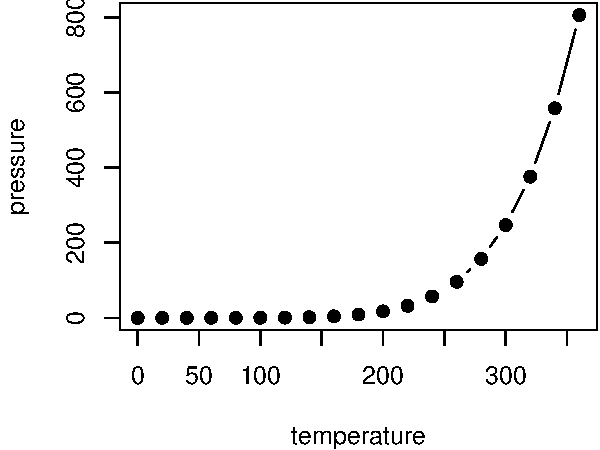
\includegraphics[width=0.8\linewidth]{260-understand-customer-needs-cross-refs_files/figure-latex/nice-fig-1} 

}

\caption{Here is a nice figure!}\label{fig:nice-fig}
\end{figure}

Don't miss Table \ref{tab:nice-tab}.

\begin{Shaded}
\begin{Highlighting}[]
\NormalTok{knitr}\SpecialCharTok{::}\FunctionTok{kable}\NormalTok{(}
  \FunctionTok{head}\NormalTok{(pressure, }\DecValTok{10}\NormalTok{), }\AttributeTok{caption =} \StringTok{\textquotesingle{}Here is a nice table!\textquotesingle{}}\NormalTok{,}
  \AttributeTok{booktabs =} \ConstantTok{TRUE}
\NormalTok{)}
\end{Highlighting}
\end{Shaded}

\begin{table}

\caption{\label{tab:nice-tab}Here is a nice table!}
\centering
\begin{tabular}[t]{rr}
\toprule
temperature & pressure\\
\midrule
0 & 0.0002\\
20 & 0.0012\\
40 & 0.0060\\
60 & 0.0300\\
80 & 0.0900\\
\addlinespace
100 & 0.2700\\
120 & 0.7500\\
140 & 1.8500\\
160 & 4.2000\\
180 & 8.8000\\
\bottomrule
\end{tabular}
\end{table}

\hypertarget{design-of-product-and-service}{%
\chapter{Design of Product and Service}\label{design-of-product-and-service}}

Once customer needs are identified, businesses develop products or services that address those needs and provide value.

Ensuring that products or services are available and accessible to customers through appropriate channels (e.g., physical stores, online platforms) is a key aspect of marketing.

\hypertarget{employee-relationships}{%
\section{Employee relationships}\label{employee-relationships}}

\hypertarget{customer-relationships}{%
\section{Customer relationships}\label{customer-relationships}}

Building and maintaining strong relationships with customers is vital. This includes providing excellent customer service, addressing feedback, and retaining loyal customers.

\hypertarget{vendor-relationships}{%
\section{Vendor relationships}\label{vendor-relationships}}

\begin{verbatim}
- > Optimizing The Value Chain
\end{verbatim}

\hypertarget{culture}{%
\section{Culture}\label{culture}}

\begin{verbatim}
- > Building A Winning Team
- > Dealing With Customer Complaints
- > Leadership As A Management Tool
- > Time Management
\end{verbatim}

\hypertarget{parts}{%
\section{Parts}\label{parts}}

You can add parts to organize one or more book chapters together. Parts can be inserted at the top of an .Rmd file, before the first-level chapter heading in that same file.

Add a numbered part: \texttt{\#\ (PART)\ Act\ one\ \{-\}} (followed by \texttt{\#\ A\ chapter})

Add an unnumbered part: \texttt{\#\ (PART\textbackslash{}*)\ Act\ one\ \{-\}} (followed by \texttt{\#\ A\ chapter})

Add an appendix as a special kind of un-numbered part: \texttt{\#\ (APPENDIX)\ Other\ stuff\ \{-\}} (followed by \texttt{\#\ A\ chapter}). Chapters in an appendix are prepended with letters instead of numbers.

\hypertarget{product-and-service-delivery}{%
\chapter{Product and Service Delivery}\label{product-and-service-delivery}}

\begin{verbatim}
- > Optimizing The Value Chain
\end{verbatim}

\hypertarget{process-design}{%
\section{Process design}\label{process-design}}

\hypertarget{distribution}{%
\section{Distribution}\label{distribution}}

\begin{verbatim}
- > Inventory Management
- > Building A Winning Team
- > Downsizing As A Cost Cutting Strategy
- > Money Ain't Everything! Smart Ways To Recognize And Reward Your Team
- > Recruiting Good People
\end{verbatim}

\hypertarget{footnotes-and-citations}{%
\section{Footnotes and citations}\label{footnotes-and-citations}}

\hypertarget{footnotes}{%
\section{Footnotes}\label{footnotes}}

Footnotes are put inside the square brackets after a caret \texttt{\^{}{[}{]}}. Like this one \footnote{This is a footnote.}.

\hypertarget{citations}{%
\section{Citations}\label{citations}}

Reference items in your bibliography file(s) using \texttt{@key}.

For example, we are using the \textbf{bookdown} package \citep{R-bookdown} (check out the last code chunk in index.Rmd to see how this citation key was added) in this sample book, which was built on top of R Markdown and \textbf{knitr} \citep{xie2015} (this citation was added manually in an external file book.bib).
Note that the \texttt{.bib} files need to be listed in the index.Rmd with the YAML \texttt{bibliography} key.

The \texttt{bs4\_book} theme makes footnotes appear inline when you click on them. In this example book, we added \texttt{csl:\ chicago-fullnote-bibliography.csl} to the \texttt{index.Rmd} YAML, and include the \texttt{.csl} file. To download a new style, we recommend: \url{https://www.zotero.org/styles/}

The RStudio Visual Markdown Editor can also make it easier to insert citations: \url{https://rstudio.github.io/visual-markdown-editing/\#/citations}

\hypertarget{sales-1}{%
\chapter{Sales}\label{sales-1}}

\begin{verbatim}
- > Features And Benefits
- > Sustaining Competitive Advantage
\end{verbatim}

\hypertarget{pricing}{%
\section{Pricing}\label{pricing}}

Determining the right price for a product or service is a crucial marketing decision. Pricing should reflect both the perceived value to the customer and the business's profitability goals.

\begin{verbatim}
- > Pricing Strategies For SMEs
\end{verbatim}

\hypertarget{promotion}{%
\section{Promotion}\label{promotion}}

Promotion involves creating awareness and interest in your products or services. This includes advertising, public relations, content marketing, and other promotional activities.

\hypertarget{brand-building}{%
\section{Brand building}\label{brand-building}}

Branding develops a unique identity and value proposition for the business and its products or services.

\begin{verbatim}
- > Branding
- > Business-To-Business Marketing
- > Classifying Your Customers
- > Converting Contacts To Sales
- > Crafting Customer Communications
- > Creating A Sales System
- > Customer Lifetime Value
- > Customer Relationship Management
- > Dealing With Customer Complaints
- > Developing Quality Marketing Materials On A Budget
- > eCommerce? What Is It? What Can It Do For My
- Business?
- > The Elevator Speech
- > eMarketing: A Plain Guide
- > Features And Benefits
- > Getting The Most Out Of Your Advertising
- > Guarantees - A Sales Opportunity
- > Improve Your Marketing ROI
- > Making A Promotions Plan
- > Perceived Indifference Disease - Are You Suffering
- From It?
- > Power Of Word Of Mouth
- > Relationship Selling - To Be Released December,
- 2003
- > Sustaining Competitive Advantage
- > Testimonials And Referrals
- > Using Offers To Win Business
- > Yellow Pages Marketing
\end{verbatim}

\hypertarget{leadership}{%
\chapter{Leadership}\label{leadership}}

\hypertarget{a-good-person-to-have-in-a-storm}{%
\section{`A Good Person to Have in a Storm'}\label{a-good-person-to-have-in-a-storm}}

refers to someone who possesses certain characteristics and qualities that make them dependable and valuable during difficult or challenging times. These characteristics include:

\begin{itemize}
\item
  Resilience: A good person in a storm remains calm and composed under pressure. They don't panic and can handle stress well.
\item
  Resourcefulness: They have the ability to find solutions and resources even when faced with limited options. They are creative problem-solvers.
\item
  Supportive: They offer emotional support and encouragement to those around them, helping to boost morale and keep people motivated.
\item
  Dependable: People can rely on them to fulfill their commitments and responsibilities, ensuring that important tasks are completed.
\item
  Leadership: They may take on a leadership role, guiding others and making decisions that benefit the group as a whole.
\item
  Adaptability: They can adjust to changing circumstances and make quick decisions when necessary.
\item
  Empathy: They show understanding and compassion for others who may be struggling during the storm.
\item
  Preparedness: They may have taken proactive steps to prepare for difficult situations, such as having necessary supplies on hand.
\item
  Positivity: They maintain a positive attitude and outlook, which can help uplift those around them.
\item
  Courage: They are not afraid to face adversity head-on and are willing to take risks to protect or assist others.
\end{itemize}

These qualities collectively make someone a valuable and reassuring presence during challenging times, whether it's a literal storm or a metaphorical one.

\hypertarget{courage-as-business-strategy}{%
\chapter{Courage as Business Strategy}\label{courage-as-business-strategy}}

An important form of courage in business is the willingness and determination to stand out from the competition by offering unique products, services, or experiences. This type of courage is essential for owners who aim to create a competitive advantage and capture the attention of their target audience.

{{[}Describe any Unique products? Unique services? Unique customer experiences?{]}}

Here are some key aspects of business courage in the context of differentiation:

\begin{itemize}
\tightlist
\item
  Challenging the Status Quo: Courageous owners are not content with following industry norms or copying competitors. They question existing practices and explore innovative ways to do things differently. They recognize that true differentiation often requires challenging conventional wisdom.
\end{itemize}

{{[}Describe some things you do that are `status quo' for your industry? Are you copying competitors? Are you following industry norms? Do you question your existing practices? Do you look for innovative ways to make your customers happier? Describe the last time you challenged conventional wisdom.{]}}

\begin{itemize}
\tightlist
\item
  Innovation: Being different begins with innovation in product, processes, or both. You need the courage to invest in research and development, experiment with new technologies and processes, and pioneer creative solutions. This will involve taking some risks and deviating from the tried-and-true.
\end{itemize}

{{[}Describe any recent innovations in product, processes, or marketing. Is your R\&D budget increasing? Describe recent creative customer solutions you've pioneered.{]}}

\begin{itemize}
\tightlist
\item
  Risk-Taking: Courageous differentiation involves calculated risk-taking. Business leaders must assess potential risks and rewards and be willing to move forward even when outcomes are uncertain. They understand that playing it safe will lead to stagnation and missed opportunities.
\end{itemize}

{{[}Describe a recent situation where you `played it safe' and missed an opportunity. Describe a recent situation where you `took a chance' when the outcome was uncertain.{]}}

\begin{itemize}
\tightlist
\item
  Long-Term Vision: Differentiation isn't just about immediate gains; it requires a long-term perspective. Courageous owners are committed to their unique value propositions and are willing to invest time and resources in building a sustainable competitive advantage.
\end{itemize}

{{[}Do you have a competitive advantage? Describe recent investments of time and resources building that advantage.{]}}

\begin{itemize}
\tightlist
\item
  Resilience: Not all attempts at differentiation will be successful, and setbacks are inevitable. Business courage means having the resilience to persevere in the face of challenges. It involves learning from failures and adapting strategies accordingly.
\end{itemize}

{{[}Describe a recent situation where you perservered in the face of challenges. Describe a recent `failure' and how you adapted your strategy accordingly.{]}}

\begin{itemize}
\tightlist
\item
  Customer-Centric: It takes more courage than you think to develop a deep understanding of customer needs and preferences. Owners must have the courage to listen to customer feedback, adapt to changing demands, and align their operations with what customers value.
\end{itemize}

{{[}Describe a recent example of when you listened to customer feedback and changed your company to address those changing demands.{]}}

\begin{itemize}
\tightlist
\item
  Marketing and Communication: Effectively communicating how and why you are different to the market requires courage and creativity. Courageous owners develop compelling messaging and branding that highlight their uniqueness. They are not afraid to be bold in their marketing efforts.
\end{itemize}

{{[}Describe a recent marketing effort that you consider `bold'.{]}}

\begin{itemize}
\tightlist
\item
  Leadership: courage always starts at the top. Business leaders must lead by example, fostering a culture of innovation, risk-taking, and differentiation within their organizations. They should encourage employees to share innovative ideas without fear of criticism.
\end{itemize}

{{[}Describe a recent example of leading by example. Describe a recent example of encouraging employees to innovate and take risks. Can your employees share innovative ideas without fear?{]}}

\begin{itemize}
\tightlist
\item
  Adaptability: Markets evolve, and customer preferences change. Courageous owners are adaptable and open to revisiting their differentiation strategies as needed. They understand that what sets them apart today may not do so in the future.
\end{itemize}

{{[}Describe how you keep your differentiation strategy `fresh'.{]}}

\begin{itemize}
\tightlist
\item
  Competitive Edge: Ultimately, differentiation through courage provides a competitive edge. It allows companies to capture market share, build brand loyalty, and thrive in competitive environments.
\end{itemize}

{{[}Describe how you are thriving now in your competitive environment.{]}}

In summary, business courage in the context of differentiation is about having the audacity to be different, the vision to see the potential rewards, and the resilience to overcome obstacles. It's a strategic mindset that sets successful companies apart and allows them to create lasting value in the marketplace.

\hypertarget{part-part-iv---what-could-possibly-go-wrong}{%
\part*{Part IV - WHAT COULD POSSIBLY GO WRONG?!!}\label{part-part-iv---what-could-possibly-go-wrong}}


Arrow-like characters in Unicode:

\begin{verbatim}
Leftwards Arrow: ← &#x2190;
Upwards Arrow: ↑ &#x2191;
Rightwards Arrow: → &#x2192;
Downwards Arrow: ↓ &#x2193;
Diagonal Arrow: ↗ &#x2197;
Diagonal Arrow: ↘ &#x2198;
Bent Arrow: ↪ &#x21AA;
Bent Arrow: ↩ &#x21A9;
\end{verbatim}

RED BOX Example of an \textbf{.rmdcaution} block.

GREEN BOX Example of an \textbf{.rmdimportant} block.

BLUE BOX Example of an \textbf{.rmdtip} block.

BLUEVIOLET BOX Example of an \textbf{.rmdwarning} block.

\hypertarget{faulty-rules-of-thumb}{%
\chapter{Faulty Rules-of-Thumb}\label{faulty-rules-of-thumb}}

{ASPIRATIONS}
{+}
{VALUE CREATION}
{+}
{COMPETITIVE STRATEGY }
{+}
{MARKET TACTICS}
{+}
{PHILOSOPY}
{+}
{OPERATIONS}
{+}
{CUSTOMERS}
{+}
{SOME LUCK}
{=}
{SUCCESS}

``I honestly beleave it is better to know nothing than two know what ain't so. Wisdom don't consist in knowing more that is true, but in knowing less that is false.''

--- paraphrased from Josh Billings (1874)

(19th-century American humorist Henry Wheeler Shaw)

{MARKETPLACE ASPIRATION: \textbf{``We want to\ldots{} be the market of choice for dairy products and produce in the tri-state area\ldots to do that we must\ldots create delighted customers.''}}

Becomes\ldots{}{\textbf{``Our Mission is to Create Delighted Customers''}}

Everyone in that enterprise knows a happy customer when they see one, and an unhappy customer when they see one. That mission statement informs people from the top of the organization chart to the bottom whether the company did a great job, or whether the value delivery system could improve.

{PHILOSOPHY:} \textbf{Rule \#1 - The Customer is Always Right. If the Customer is Ever Wrong, See Rule \#1''}

{MARKETPLACE STRATEGY:} \textbf{Offer freshest produce and dairy products at the lowest cost with an in-store experience that leaves customers saying ``WOW!'' The in-store experience will be very difficult for competitors to duplicate.}

{MARKETPLACE TACTICS:} \textbf{Produce our own in-store, super-high-quality, super-low-cost dairy products. Buy produce directly from farmers from coast-to-coast to guarantee quality and freshness (and cut out the middleman). Insist on highest quality on all other store products. Sell fewer products but buy in higher quantities and pass the savings on. This alone will make us meaningfully different than the competition.}

{BECOMES:} \textbf{``Our mission is to create delighted customers.''}

\hypertarget{part-part-v---other-matters}{%
\part*{Part V - OTHER MATTERS}\label{part-part-v---other-matters}}


\hypertarget{ownership-issues}{%
\chapter{Ownership Issues}\label{ownership-issues}}

\begin{verbatim}
- > Failing To Plan Is Planning To Fail
- > Working ON Rather Than IN Your Business
- > Professionalizing The Family Business
- > Starting Up A Business
- > Failing To Plan Is Planning To Fail
- > Trademarks And Patents
- > Franchising
- > SWOT: Your Business Health Check
- > Downsizing As A Cost Cutting Strategy   
\end{verbatim}

\hypertarget{finance}{%
\chapter{Finance}\label{finance}}

\begin{verbatim}
- > Business Valuation - To Be Released
- > Key Performance Indicators - Tools For Business
- > Performance Management
- > Managing Your Accounts Receivable
- > Managing Your Cash Flow
- > Smart Ways To Control Costs
- > Starting Up A Business
\end{verbatim}

\hypertarget{sharing-your-book}{%
\chapter{Sharing your book}\label{sharing-your-book}}

\hypertarget{publishing}{%
\section{Publishing}\label{publishing}}

HTML books can be published online, see: \url{https://bookdown.org/yihui/bookdown/publishing.html}

\hypertarget{pages}{%
\section{404 pages}\label{pages}}

By default, users will be directed to a 404 page if they try to access a webpage that cannot be found. If you'd like to customize your 404 page instead of using the default, you may add either a \texttt{\_404.Rmd} or \texttt{\_404.md} file to your project root and use code and/or Markdown syntax.

\hypertarget{metadata-for-sharing}{%
\section{Metadata for sharing}\label{metadata-for-sharing}}

Bookdown HTML books will provide HTML metadata for social sharing on platforms like Twitter, Facebook, and LinkedIn, using information you provide in the \texttt{index.Rmd} YAML. To setup, set the \texttt{url} for your book and the path to your \texttt{cover-image} file. Your book's \texttt{title} and \texttt{description} are also used.

This \texttt{bs4\_book} provides enhanced metadata for social sharing, so that each chapter shared will have a unique description, auto-generated based on the content.

Specify your book's source repository on GitHub as the \texttt{repo} in the \texttt{\_output.yml} file, which allows users to view each chapter's source file or suggest an edit. Read more about the features of this output format here:

\url{https://pkgs.rstudio.com/bookdown/reference/bs4_book.html}

Or use:

\begin{Shaded}
\begin{Highlighting}[]
\NormalTok{?bookdown}\SpecialCharTok{::}\NormalTok{bs4\_book}
\end{Highlighting}
\end{Shaded}

\hypertarget{gif-library-as-of-2023-12-06}{%
\chapter{GIF LIBRARY AS OF 2023-12-06}\label{gif-library-as-of-2023-12-06}}

\includegraphics{gif/5_of_5_stars.gif}
\includegraphics{gif/baby_learning.gif}
\includegraphics{gif/baby-elephant-hugs.gif}
\includegraphics{gif/baby-elephant-river-run.gif}
\includegraphics{gif/baby-throwing-money-out-window.gif}
\includegraphics{gif/bending_over_backwards_handshake.gif}
\includegraphics{gif/boss_dangling_carrot_for_employee.gif}
\includegraphics{gif/boxer_bouncing_at_door.gif}
\includegraphics{gif/brad_pulling_random_levers.gif}
\includegraphics{gif/breaking-what-already-works-bird-and-puzzle.gif}
\includegraphics{gif/bright_idea_lightbulb.gif}
\includegraphics{gif/bullseye_target_miss.gif}
\includegraphics{gif/cardiogram_heart_signal.gif}
\includegraphics{gif/_data_appearing.gif}
\includegraphics{gif/flashing_lights_sign.gif}
\includegraphics{gif/caught_in_gears.gif}
\includegraphics{gif/chicken-loves-boy.gif}
\includegraphics{gif/child-walks-thr-spinning-hoop.gif}
\includegraphics{gif/clashing-methods-bubble_people.gif}
\includegraphics{gif/clever-child-entrepreneur.gif}
\includegraphics{gif/clones1.gif}
\includegraphics{gif/clones2.gif}
\includegraphics{gif/clones3.gif}
\includegraphics{gif/combined-msr-growth-curves.gif}
\includegraphics{gif/pointing_at_chalkboard.gif}
\includegraphics{gif/puts_on_a_happy_face.gif}
\includegraphics{gif/Only.gif}
\includegraphics{gif/disappointed-zoey.gif}
\includegraphics{gif/erasable_sad_face.gif}
\includegraphics{gif/divorce.gif}
\includegraphics{gif/doctor_listening_heart.gif}
\includegraphics{gif/doesnt-fit-disaster.gif}
\includegraphics{gif/dog-pals.gif}
\includegraphics{gif/donald-duck-laughing-at-others.gif}
\includegraphics{gif/ekg.gif}
\includegraphics{gif/enthusiasm_1SjObB0Y07mg0.gif}
\includegraphics{gif/enthusiasm-steph.gif}
\includegraphics{gif/enthusiasm-student-cheering.gif}
\includegraphics{gif/enthusiastic-steph.gif}
\includegraphics{gif/entusiasm1.gif}
\includegraphics{gif/figure_looking_observing.gif}
\includegraphics{gif/figure_oiling_gears.gif}
\includegraphics{gif/follow-the-crowd-mentality.gif}
\includegraphics{gif/hands_giving_keys_to_buyer.gif}
\includegraphics{gif/homer-pounds-puzzle-pieces.gif}
\includegraphics{gif/idris-frustrated.gif}
\includegraphics{gif/inflated_dance_man.gif}
\includegraphics{gif/its-cold.gif}
\includegraphics{gif/pondering_board.gif}
\includegraphics{gif/monday.gif}
\includegraphics{gif/moving_target_on_ground.gif}
\includegraphics{gif/my-job-in-solving-the-puzzle.gif}
\includegraphics{gif/old-man-working-flea-market.gif}
\includegraphics{gif/businessman_ponder_question.gif}
\includegraphics{gif/pondering_two_thoughts.gif}
\includegraphics{gif/power-pulsing.gif}
\includegraphics{gif/printing-newspapers.gif}
\includegraphics{gif/push_5_of_5_stars.gif}
\includegraphics{gif/puzzle-parts-dont-fit.gif}
\includegraphics{gif/stick_figure_question_answer.gif}
\includegraphics{gif/back_and_forth_questions.gif}
\includegraphics{gif/reaching_for_the_stars.gif}
\includegraphics{gif/red-raincoat-in-crowd.gif}
\includegraphics{gif/roller_coaster_fun.gif}
\includegraphics{gif/sesame-brought-to-you-by-letter.gif}
\includegraphics{gif/should-fit-but-doesnt.gif}
\includegraphics{gif/signs_rise_questions.gif}
\includegraphics{gif/stand-out-in-crowd.gif}
\includegraphics{gif/stick_figure_bailing_water.gif}
\includegraphics{gif/stick_figure_cranking_money.gif}
\includegraphics{gif/pt_answer.gif}
\includegraphics{gif/thank-you-baby-elephant-hugs.gif}
\includegraphics{gif/thank-you-baby-elephant-river-run.gif}
\includegraphics{gif/thank-you-boxer-applause.gif}
\includegraphics{gif/thank-you-boy-hugs-chicken.gif}
\includegraphics{gif/thank-you-bubble-people.gif}
\includegraphics{gif/thank-you-bulldog-on-jetski.gif}
\includegraphics{gif/thank-you-child-walks-by-spinning-hoop.gif}
\includegraphics{gif/thank-you-dog-pals.gif}
\includegraphics{gif/thank-you-elvis.gif}
\includegraphics{gif/thank-you-happy-puzzling.gif}
\includegraphics{gif/thank-you-sam-elliot.gif}
\includegraphics{gif/turn_on_off_brain_anim.gif}
\includegraphics{gif/turtle_helping_turtle.gif}
\includegraphics{gif/what-others-promise-ideal-world-puzzle-pieces.gif}
\includegraphics{gif/whats-going-on-here-croods.gif}
\includegraphics{gif/woman_back_and_forth_questions.gif}
\includegraphics{gif/working_hard_for_the_money.gif}
\includegraphics{gif/zombies.gif}
NA

\hypertarget{img-library-as-of-2023-12-06}{%
\chapter{IMG LIBRARY AS OF 2023-12-06}\label{img-library-as-of-2023-12-06}}

\includegraphics{img/5-star-rating.jpg}
\includegraphics{img/6-sigma-round-hole-square-peg-text.png}
\includegraphics{img/agile-round_hole_square_peg.png}
\includegraphics{img/all-4-quadrants-with-dots.png}
\includegraphics{img/architects-meeting.jpg}
\includegraphics{img/arrogant-imogi.png}
\includegraphics{img/be-unique-red-paper-plane.jpg}
\includegraphics{img/best-practices-fail.png}
\includegraphics{img/best-practices-round_hole_square_peg.png}
\includegraphics{img/blank-all-4-quadrants.png}
\includegraphics{img/blank-minimum-sales-table-rows1-6.png}
\includegraphics{img/bull_by_the_horns.png}
\includegraphics{img/cart-before-horse.jpg}
\includegraphics{img/certification.png}
\includegraphics{img/command-and-control-heirarchy.jpg}
\includegraphics{img/wordcloud.png}
\includegraphics{img/common-journey-mermaid.png}
\includegraphics{img/confused.woman.jpg}
\includegraphics{img/deming-chain-reaction.png}
\includegraphics{img/Reaction.png}
\includegraphics{img/demo-share-again.png}
\includegraphics{img/dog-at-vet-office.jpg}
\includegraphics{img/education.cost.png}
\includegraphics{img/elderly-businessman.jpg}
\includegraphics{img/example-normalized-stmt.png}
\includegraphics{img/figure-out-what-works.jpg}
\includegraphics{img/financial.security.png}
\includegraphics{img/food.water.shelter.jpg}
\includegraphics{img/frustrated-customer.jpg}
\includegraphics{img/furniture.jpg}
\includegraphics{img/global-travel.jpg}
\includegraphics{img/Goose-Creek-Tower-Alaska.png}
\includegraphics{img/happy-customer.jpg}
\includegraphics{img/head-for-business-1.png}
\includegraphics{img/health.insurance.png}
\includegraphics{img/heart.health.png}
\includegraphics{img/home.png}
\includegraphics{img/ideal-business-launch-diagram-85.png}
\includegraphics{img/ideal-business-launch-diagram-v2.png}
\includegraphics{img/ideal-business-launch-diagram.png}
\includegraphics{img/ideal-business-launch-flowchart.png}
\includegraphics{img/japanese-logos-of-the-worlds-most-admired-companies.jpg}
\includegraphics{img/john-seddon.jpg}
\includegraphics{img/Mack\textquotesingle{}.jpeg}
\includegraphics{img/kent-billingsley-book.jpg}
\includegraphics{img/Logo.jpeg}
\includegraphics{img/loaning.money.png}
\includegraphics{img/losing-the-thread-weird-stacked-apts.jpg}
\includegraphics{img/losing-the-thread-winchester-house.jpg}
\includegraphics{img/M.starting.at.30.ggplot.static.png}
\includegraphics{img/M.starting.at.35.ggplot.static.png}
\includegraphics{img/M.starting.at.40.ggplot.static.png}
\includegraphics{img/M.starting.at.45.ggplot.static.png}
\includegraphics{img/M.starting.at.50.ggplot.static.png}
\includegraphics{img/man-making-decision.jpg}
\includegraphics{img/million.starting.at.30.ggplot.png}
\includegraphics{img/minimum-sales-table-complete-with-amounts.png}
\includegraphics{img/minimum-sales-table-rows1-1.png}
\includegraphics{img/minimum-sales-table-rows1-2.png}
\includegraphics{img/minimum-sales-table-rows1-3.png}
\includegraphics{img/minimum-sales-table-rows1-4.png}
\includegraphics{img/mistake-math.jpg}
\includegraphics{img/multiple-layers-of-management.jpg}
\includegraphics{img/north-star-circumpolar.jpg}
\includegraphics{img/north-star-lighthouse.jpg}
\includegraphics{img/percentages.piechart.jpg}
\includegraphics{img/porter-generic-strategies-diagram.jpg}
\includegraphics{img/porters-competitive-strategies.jpeg}
\includegraphics{img/profit-finger-on-graph.jpg}
\includegraphics{img/puppy-vet-exam.jpg}
\includegraphics{img/quadrants1and4.png}
\includegraphics{img/quadrants2and3.png}
\includegraphics{img/required-salary-table-complete.png}
\includegraphics{img/samsung-logo-icon-.png}
\includegraphics{img/secure.home.png}
\includegraphics{img/servant-leadearship-round_hole_square_peg.png}
\includegraphics{img/Sony-Logo.png}
\includegraphics{img/spaniel-in-hospital.jpg}
\includegraphics{img/static-vet-flow-before.png}
\includegraphics{img/swart-cpa.jpg}
\includegraphics{img/Photo.png}
\includegraphics{img/talking-with-customers.jpg}
\includegraphics{img/true-north-compass.jpg}
\includegraphics{img/true-north-diagram-65.jpeg}
\includegraphics{img/true-north-diagram-65.png}
\includegraphics{img/true-north-diagram-85.png}
\includegraphics{img/true-north-diagram.png}
\includegraphics{img/unique-1-yellow-locker.jpg}
\includegraphics{img/unique-red-paper-plane-on-black.png}
\includegraphics{img/WED-it-will-not-suffice.png}
\includegraphics{img/House1.jpg}
\includegraphics{img/House.jpg}
\includegraphics{img/woman-thinking.png}
NA

  \bibliography{book.bib,packages.bib}

\backmatter
\printindex

\end{document}
